\documentclass{template/class}

\usepackage[T1]{fontenc}

\usepackage{parskip}

\usepackage{titlesec}
\titlespacing{\section}{0pt}{3.3ex}{2ex}
\titlespacing{\subsection}{0pt}{3.3ex}{1.65ex}
\titlespacing{\subsubsection}{0pt}{3.3ex}{1ex}
\usepackage{fancyhdr}
\fancyhf{}

\usepackage[
    colorlinks=true,
    linkcolor=black,
    citecolor=black
]{hyperref}

\usepackage{biblatex}
\bibliography{bibliography}

\usepackage{graphicx}
\graphicspath{{./images/}}
\usepackage{transparent}
\usepackage{eso-pic}

\usepackage{tabularx}
\usepackage{colortbl}
\usepackage{longtable}

\usepackage{fix-cm}

\newcommand\numfontsize{\@setfontsize\Huge{200}{60}}

\newcommand{\hsp}{\hspace{0pt}}

\makeatletter
\renewcommand*\cleardoublepage{
    \clearpage
    \if@twoside
        \ifodd\c@page\else\null
            \AddToShipoutPicture*\backgroundbl
            \thispagestyle{empty}\newpage
            \if@twocolumn
                \hbox{}
                \newpage
            \fi
        \fi
    \fi
}
\makeatother

\definecolor{polimiblue}{cmyk}{.4,.1,0,.4}

\titleformat{\chapter}[hang]{\fontsize{50}{20}\selectfont\bfseries\filright}{
    \textcolor{polimiblue}
    \thechapter\hsp\hspace{2mm}\textcolor{polimiblue}{|   }
    \hsp
}{0pt}{\huge\bfseries\textcolor{polimiblue}}

\titleformat{\section}
{\color{polimiblue}\normalfont\Large\bfseries}
{\color{polimiblue}\thesection.}{1em}{}

\titleformat{\subsection}
{\color{polimiblue}\normalfont\large\bfseries}
{\color{polimiblue}\thesubsection.}{1em}{}

\titleformat{\subsubsection}
{\color{polimiblue}\normalfont\large\bfseries}
{\color{polimiblue}\thesubsubsection.}{1em}{}

\captionsetup[table]{labelfont={color=polimiblue}}
\captionsetup[figure]{labelfont={color=polimiblue}}


\begin{document}

\frontmatter

\puttitle{
    title=Students\&Companies,
    subtitle=Design Document,
    authors=Andrea Carrara\\and Federica Currò Dossi,
    date=7th of January 2025
}

\tableofcontents

\mainmatter
\setcounter{page}{1}

\chapter{Introduction}
This chapter provides essential background information about the design document, including its purpose, scope and structure.
It also introduces key terminology and references needed for understanding the technical content that follows.

\section{Purpose}
The purpose of the following document is to present a detailed design description of Students\&Companies.
It provides developers with implementation guidelines while serving as a technical agreement between customers and contractors.
The document transforms the requirements and specifications from the requirements analysis and specification document \cite{carraracurrodossi2024} into concrete architectural decisions, describing the system's components and their interactions.
It outlines the design patterns, technical interfaces and deployment strategies that will guide the development team in building a robust platform that fulfills stakeholder needs.
Additionally, it establishes a clear roadmap for implementation and testing phases, ensuring that the final system aligns with both technical requirements and business objectives.

\section{Scope}
Students\&Companies is designed to bridge the gap between academic education and practical workplace experience.
The platform facilitates the internship matching process by enabling students to create detailed profiles with CVs and preferences, while companies can post comprehensive internship opportunities including project details, required skills and terms.
S\&C features personalized recommendations through statistical analysis, manages the entire selection process from interviews to final outcome and provides tools for monitoring ongoing internships.
Additionally, universities can oversee the progress of their students, ensuring quality and addressing concerns that arise during the internships.
For a comprehensive overview of the platform's functionalities and requirements, please refer to the requirements analysis and specification document \cite{carraracurrodossi2024}.

\section{Glossary}
This table contains the key definitions, acronyms and abbreviations used in the document.

\renewcommand{\arraystretch}{1.5}
\begin{longtable}{|c|p{8.5cm}|}
    \hline \rowcolor{polimiblue!40}
    \textbf{ID} & \textbf{Description} \\ \hline
    S\&C & Students\&Companies \\ \hline
    US & University student \\ \hline
    IN & Internship job \\ \hline
    PO & Internship position \\ \hline
    CO & Company \\ \hline
    UN & University \\ \hline
    CV & Curriculum vitae \\ \hline
    Match & A US and a CO declare interest in each other \\ \hline
    Contact & Selection process and internship progress \\ \hline
\caption{Glossary}
\end{longtable}

\section{Reference Documents}
The document follows Professor Di Nitto's project assignment structure \cite{dinitto2024}.

\section{Document Structure}
This document describes the design specification for Students\&Companies, following an architecture-centric approach that progresses from system-wide design decisions to specific implementation details.
It is organized into seven chapters, each providing increasingly detailed technical information needed for implementation.

\subsubsection{Introduction}
The first chapter establishes the foundation of the design document through purpose and scope definitions, provides a comprehensive glossary, lists reference documents and explains the document's organization.

\subsubsection{Architectural Design}
The second chapter presents the system's architecture through multiple views: an overview of components and their interactions, detailed component descriptions, deployment specifications, runtime behavior illustrations, component interfaces and the rationale behind architectural styles and patterns.

\subsubsection{User Interface Design}
The third chapter details the user interface through mockups and interaction flows, covering each user category's specific interface requirements and presenting key screens and navigation patterns.

\subsubsection{Requirements Traceability}
The fourth chapter establishes clear links between the requirements from the requirements analysis and specification document \cite{carraracurrodossi2024} and their corresponding design elements, demonstrating how architectural decisions satisfy functional and non-functional requirements.

\subsubsection{Implementation, Integration and Test Plan}
The fifth chapter provides a comprehensive roadmap for system realization, detailing the implementation order of components, their integration strategy and the testing methodology to ensure system quality.

\subsubsection{Workload}
The sixth chapter quantifies each writer's time investment in the design document.


\chapter{Architectural Design}
This chapter provides a detailed architectural design of Students\&Companies, starting with a high-level overview of the system's design choices and their rationale.
It then explores the component view, illustrating major system modules and their interactions using various UML diagrams.
A deployment view follows, showing how software components distribute across hardware nodes.
Runtime views are then presented through sequence diagrams depicting key system operations.
The chapter concludes with a discussion of chosen architectural styles, patterns and other significant design decisions.

\section{Overview}
Students\&Companies requires an architecture that can efficiently handle the complex interactions between students, companies and universities while ensuring system scalability and data security.
The platform adopts a three-tier client-server architecture, separating presentation, application logic and data management into distinct layers.
This section provides an overview of the application of this architecture to the problem at hand, while a more general discussion of the architectural style belongs in later sections.

\subsubsection{Presentation Tier}
At the presentation tier, the web app serves as the user interface, allowing S\&C to be accessed by users through their browsers.
The app is responsive, ensuring accessibility across various devices while maintaining a consistent user experience.

\subsubsection{Application Tier}
The application tier consists of three server components.

The web server handles incoming client requests, managing user sessions and providing load balancing capabilities to distribute traffic effectively across multiple instances of the application server.
The application server contains the core business logic, processing user requests to coordinate the entire internship lifecycle from application to completion.

The mail server manages the email workflow, determining when to send notifications for registration confirmations, selection updates or internship comments.
For actual email delivery, the mail server integrates with an external email provider that handles the delivery infrastructure, ensuring reliable communication.

\subsubsection{Data Tier}
The data tier employs a DBMS server to store and manage all system data.
This includes user profiles, internship positions, ongoing matches, selection processes and internship records.
The DBMS server provides structured data storage with mechanisms for maintaining integrity through transaction management and constraint enforcement, optimizing query performance through indexing and caching, and implementing access controls and encryption for sensitive user data.

Overall, this architecture enables efficient data flow while maintaining scalability and security.
When a user interacts with the web app, their request flows through the web server to one of the application server instances, which processes it leveraging the data from the DBMS server and triggers notifications through the mail server when necessary.

\begin{figure}[h]
    \centering
    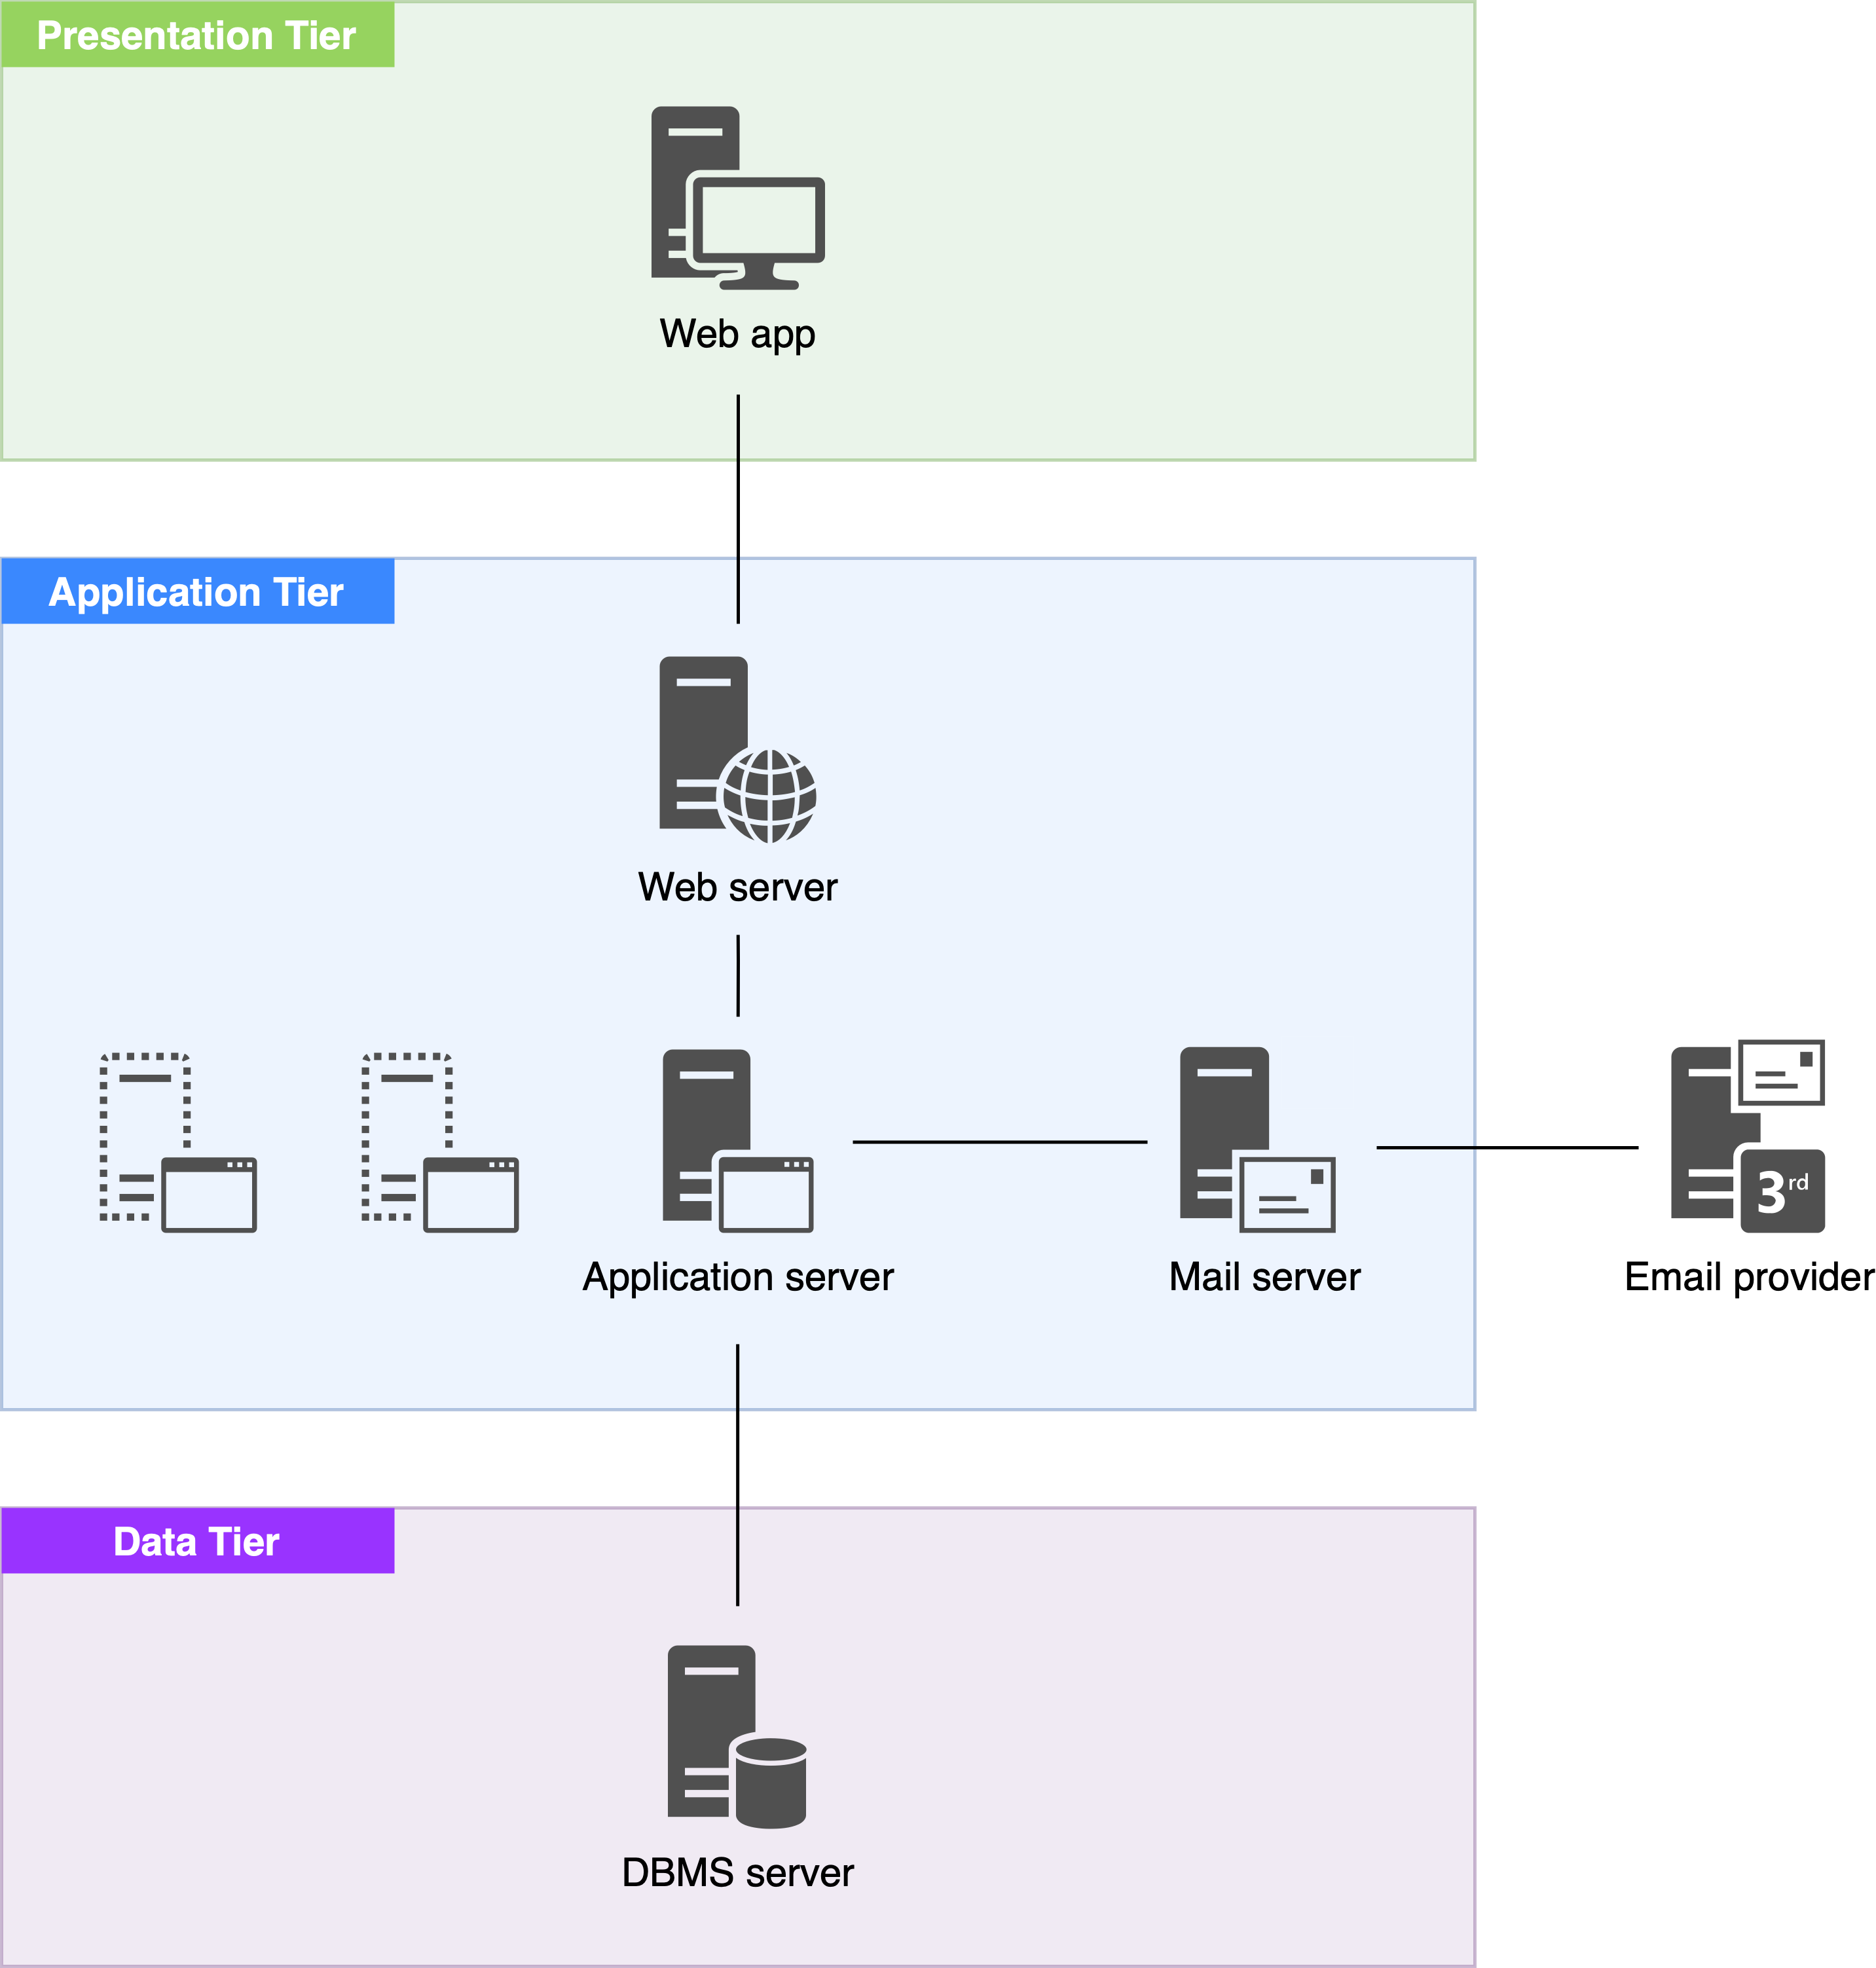
\includegraphics[width=14cm]{images/architecture.png}
    \caption{Architecture}
\end{figure}

\section{Component View}
This section illustrates the logical organization of Students\&Companies by breaking down the system into its major software modules and mapping their relationships.
Using a series of increasingly detailed UML diagrams, the component view first presents a high-level view showing the system elements and their interactions.
It then dives into individual components, examining their low-level structures, responsibilities and interfaces, with particular attention to how they collaborate to implement the platform's functionality.

\subsection{High-Level View}
The high-level diagram below shows the components of Students\&Companies and their interactions.
The system exposes six distinct interfaces to the web app, each corresponding to a specific domain of functionality that will be further discussed in the next section.

\begin{figure}[h]
    \centering
    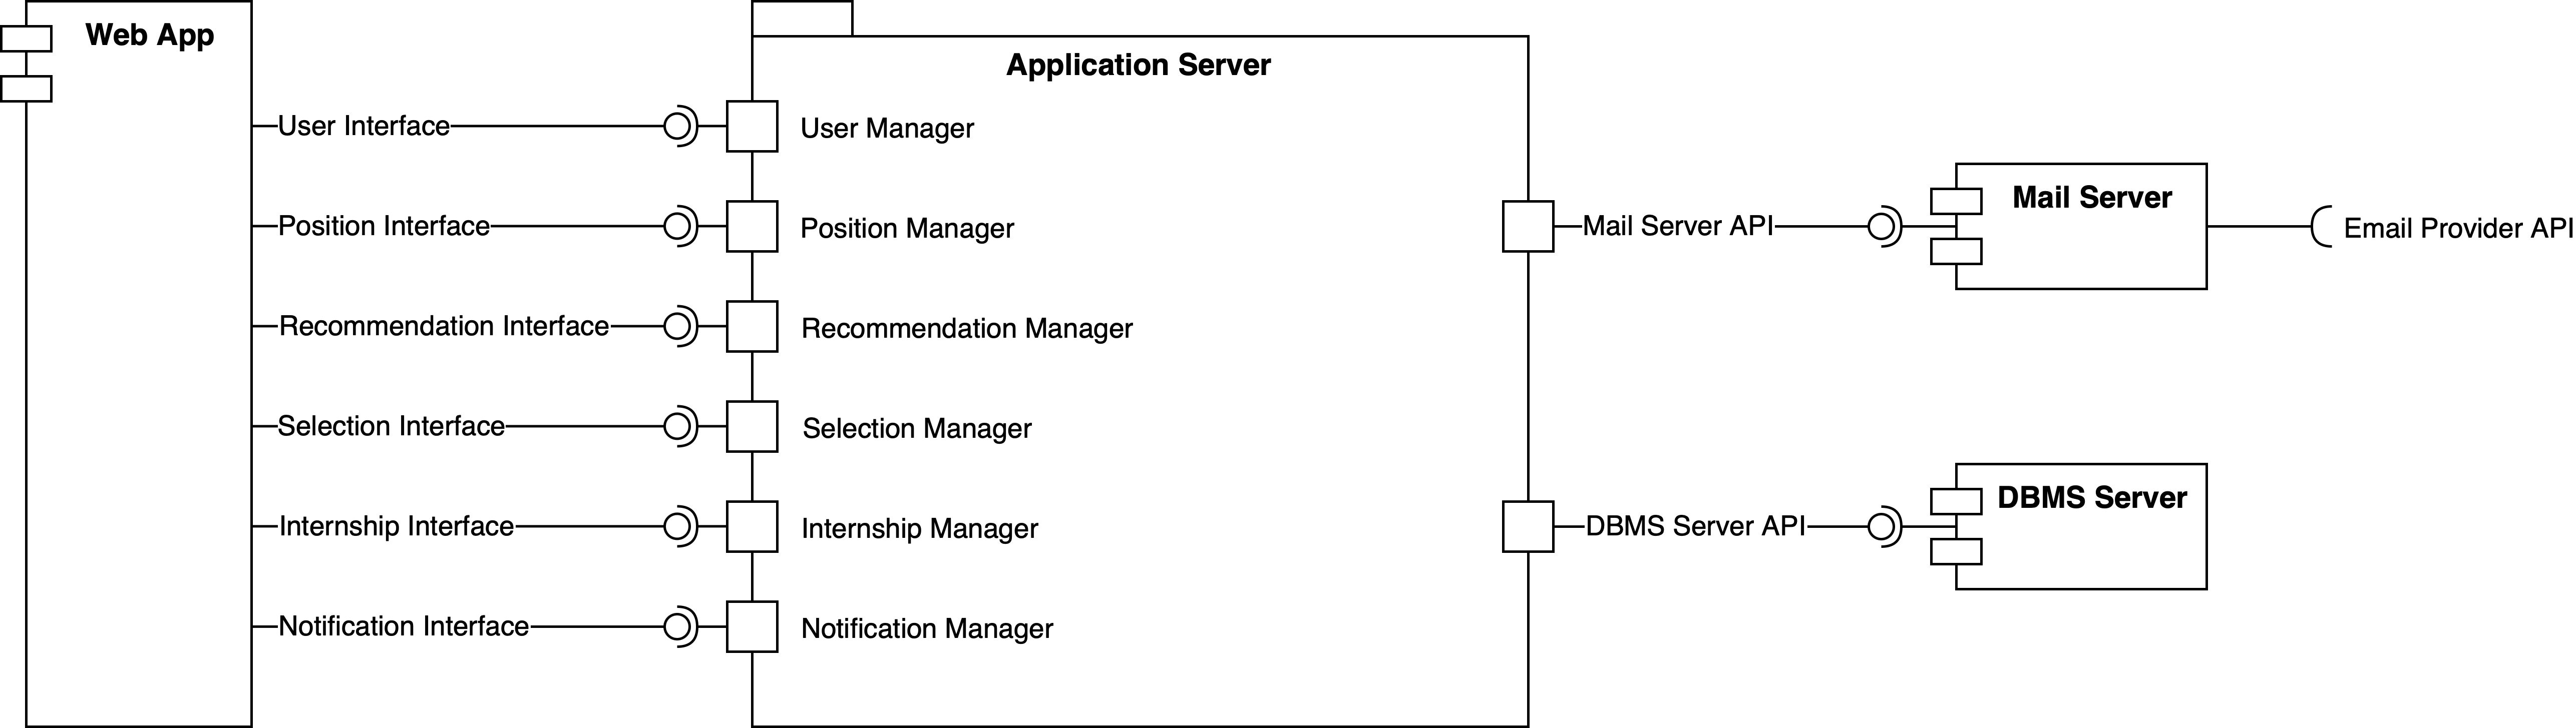
\includegraphics[width=16cm]{images/component-view/high-level.png}
    \caption{High-level component view}
\end{figure}

\subsection{Low-Level View}
The low-level view below builds upon the high-level diagram above by providing a detailed representation of the internal architecture of the application server.
The codebase is structured according to the model-view-controller pattern.
In this architecture, the model acts as the core data structure of the system, representing and managing the content of the database.
In turn, managers act as controllers, bridging the model and the external interfaces, which serve as the entry points for users, ensuring a clean separation of concerns that makes the system modular, scalable and maintainable.

\begin{figure}[ht]
    \centering
    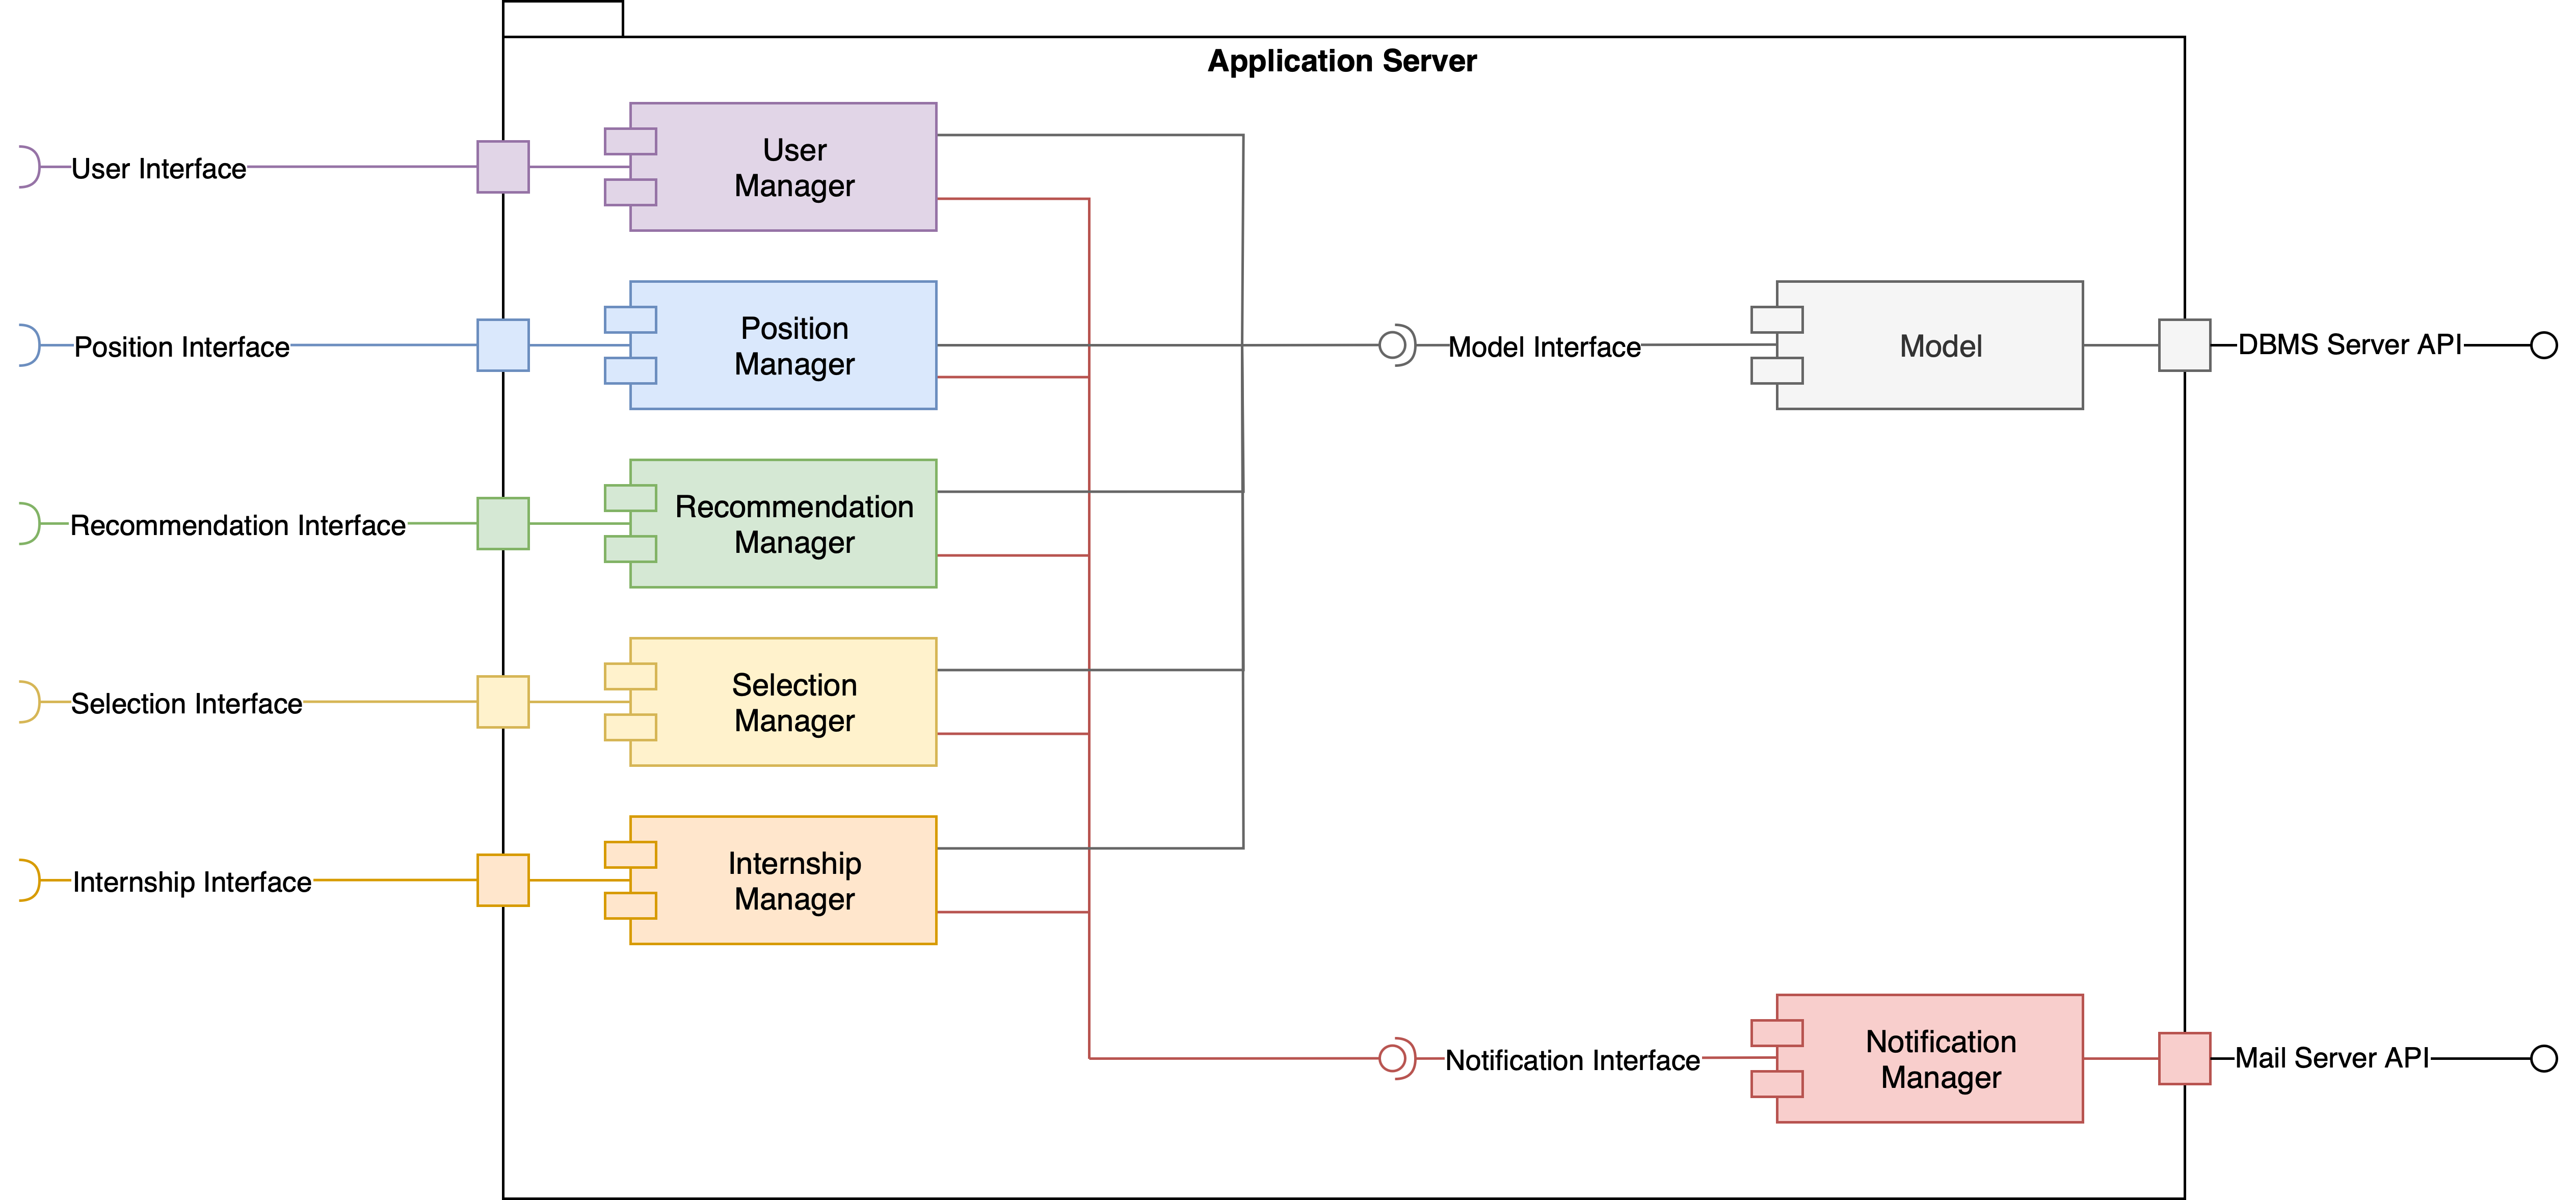
\includegraphics[width=16cm]{images/component-view/low-level.png}
    \caption{Low-level component view}
\end{figure}

Each manager is organized into multiple submanagers, which encapsulate specific functionalities within its domain.
These submanagers allow the managers to remain focused on their broader responsibilities while delegating finer tasks.
The following subsections delve into each manager, describing its role and breaking down its submanagers.

\subsubsection{User Manager}
The user interface serves as the bridge between users and the user manager, channeling requests related to account creation, authentication and management.

\begin{figure}[ht]
    \centering
    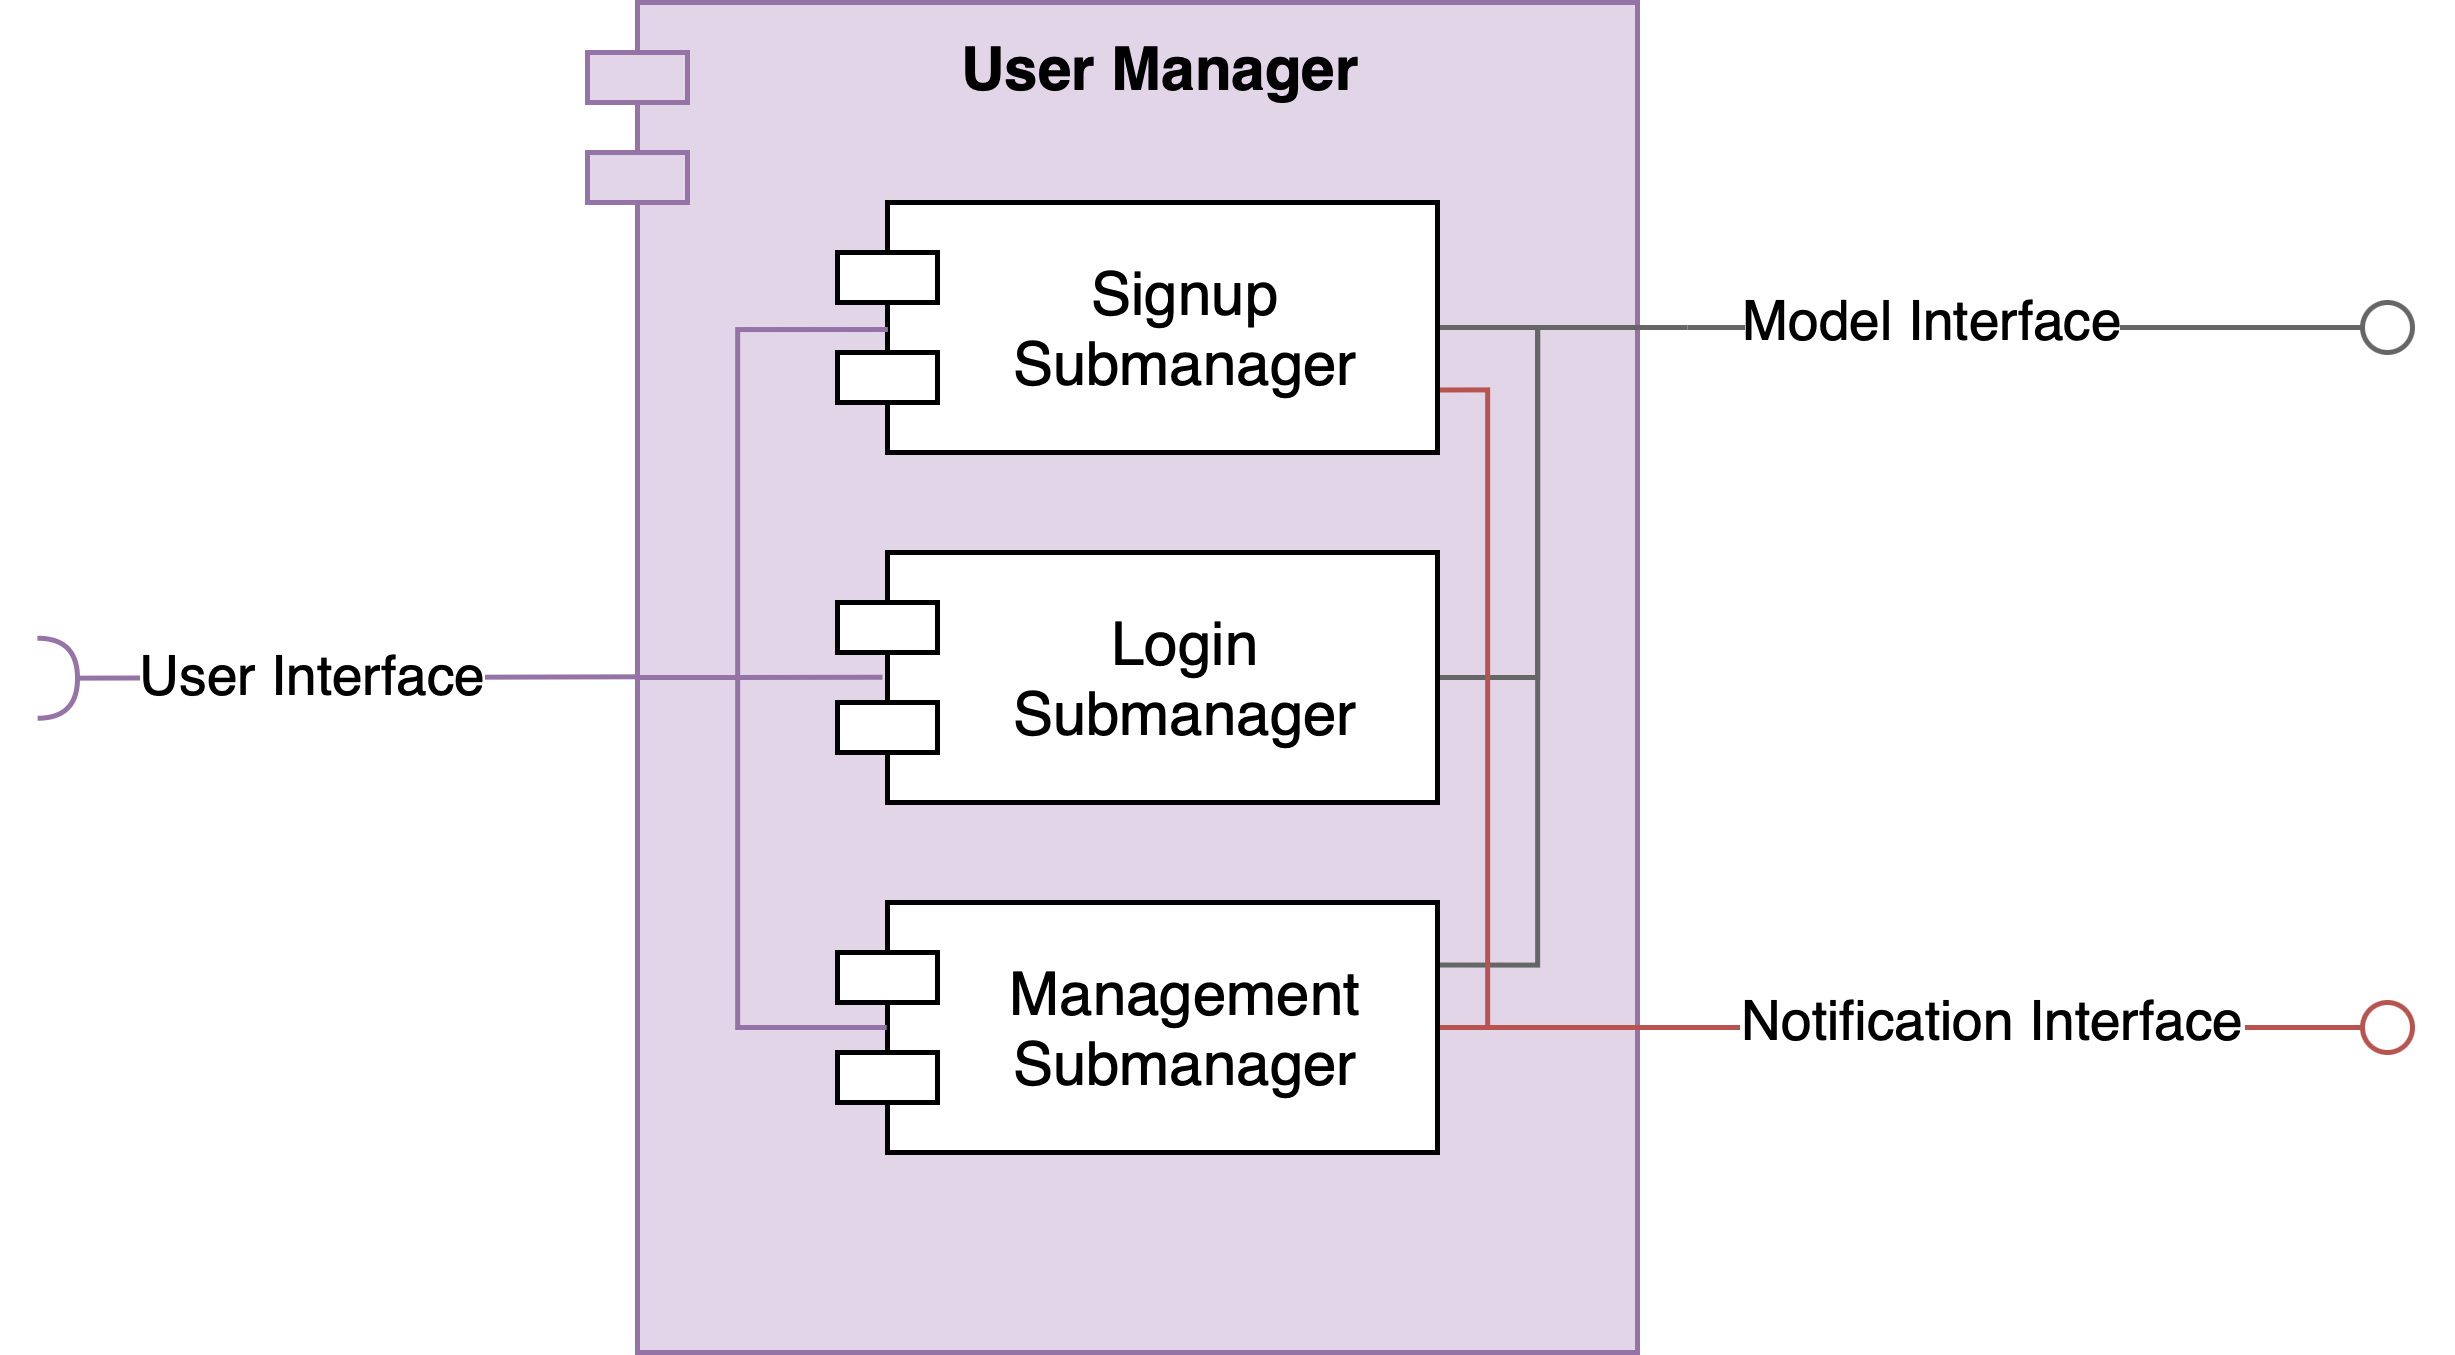
\includegraphics[width=11cm]{images/managers/user.png}
    \caption{User manager}
\end{figure}

The user signup submanager handles user onboarding by validating fields and enforcing rules like password length.
It securely integrates new users into the system while delegating confirmation emails to the notification manager.

The user login submanager supports user logins, validating credentials and issuing tokens for secure session management.
It also ensures expired tokens are revoked.

The user management submanager supports users in updating their profiles, including editing preferences and uploading CVs, validating and storing changes.
Additionally, it provides an option for account deletion.

\subsubsection{Position Manager}
The position interface acts as the portal for managing internship postings, funneling requests from both companies and students to the position manager.
This manager ensures that opportunities are validated, maintained and accessible to all relevant users.

\begin{figure}[h]
    \centering
    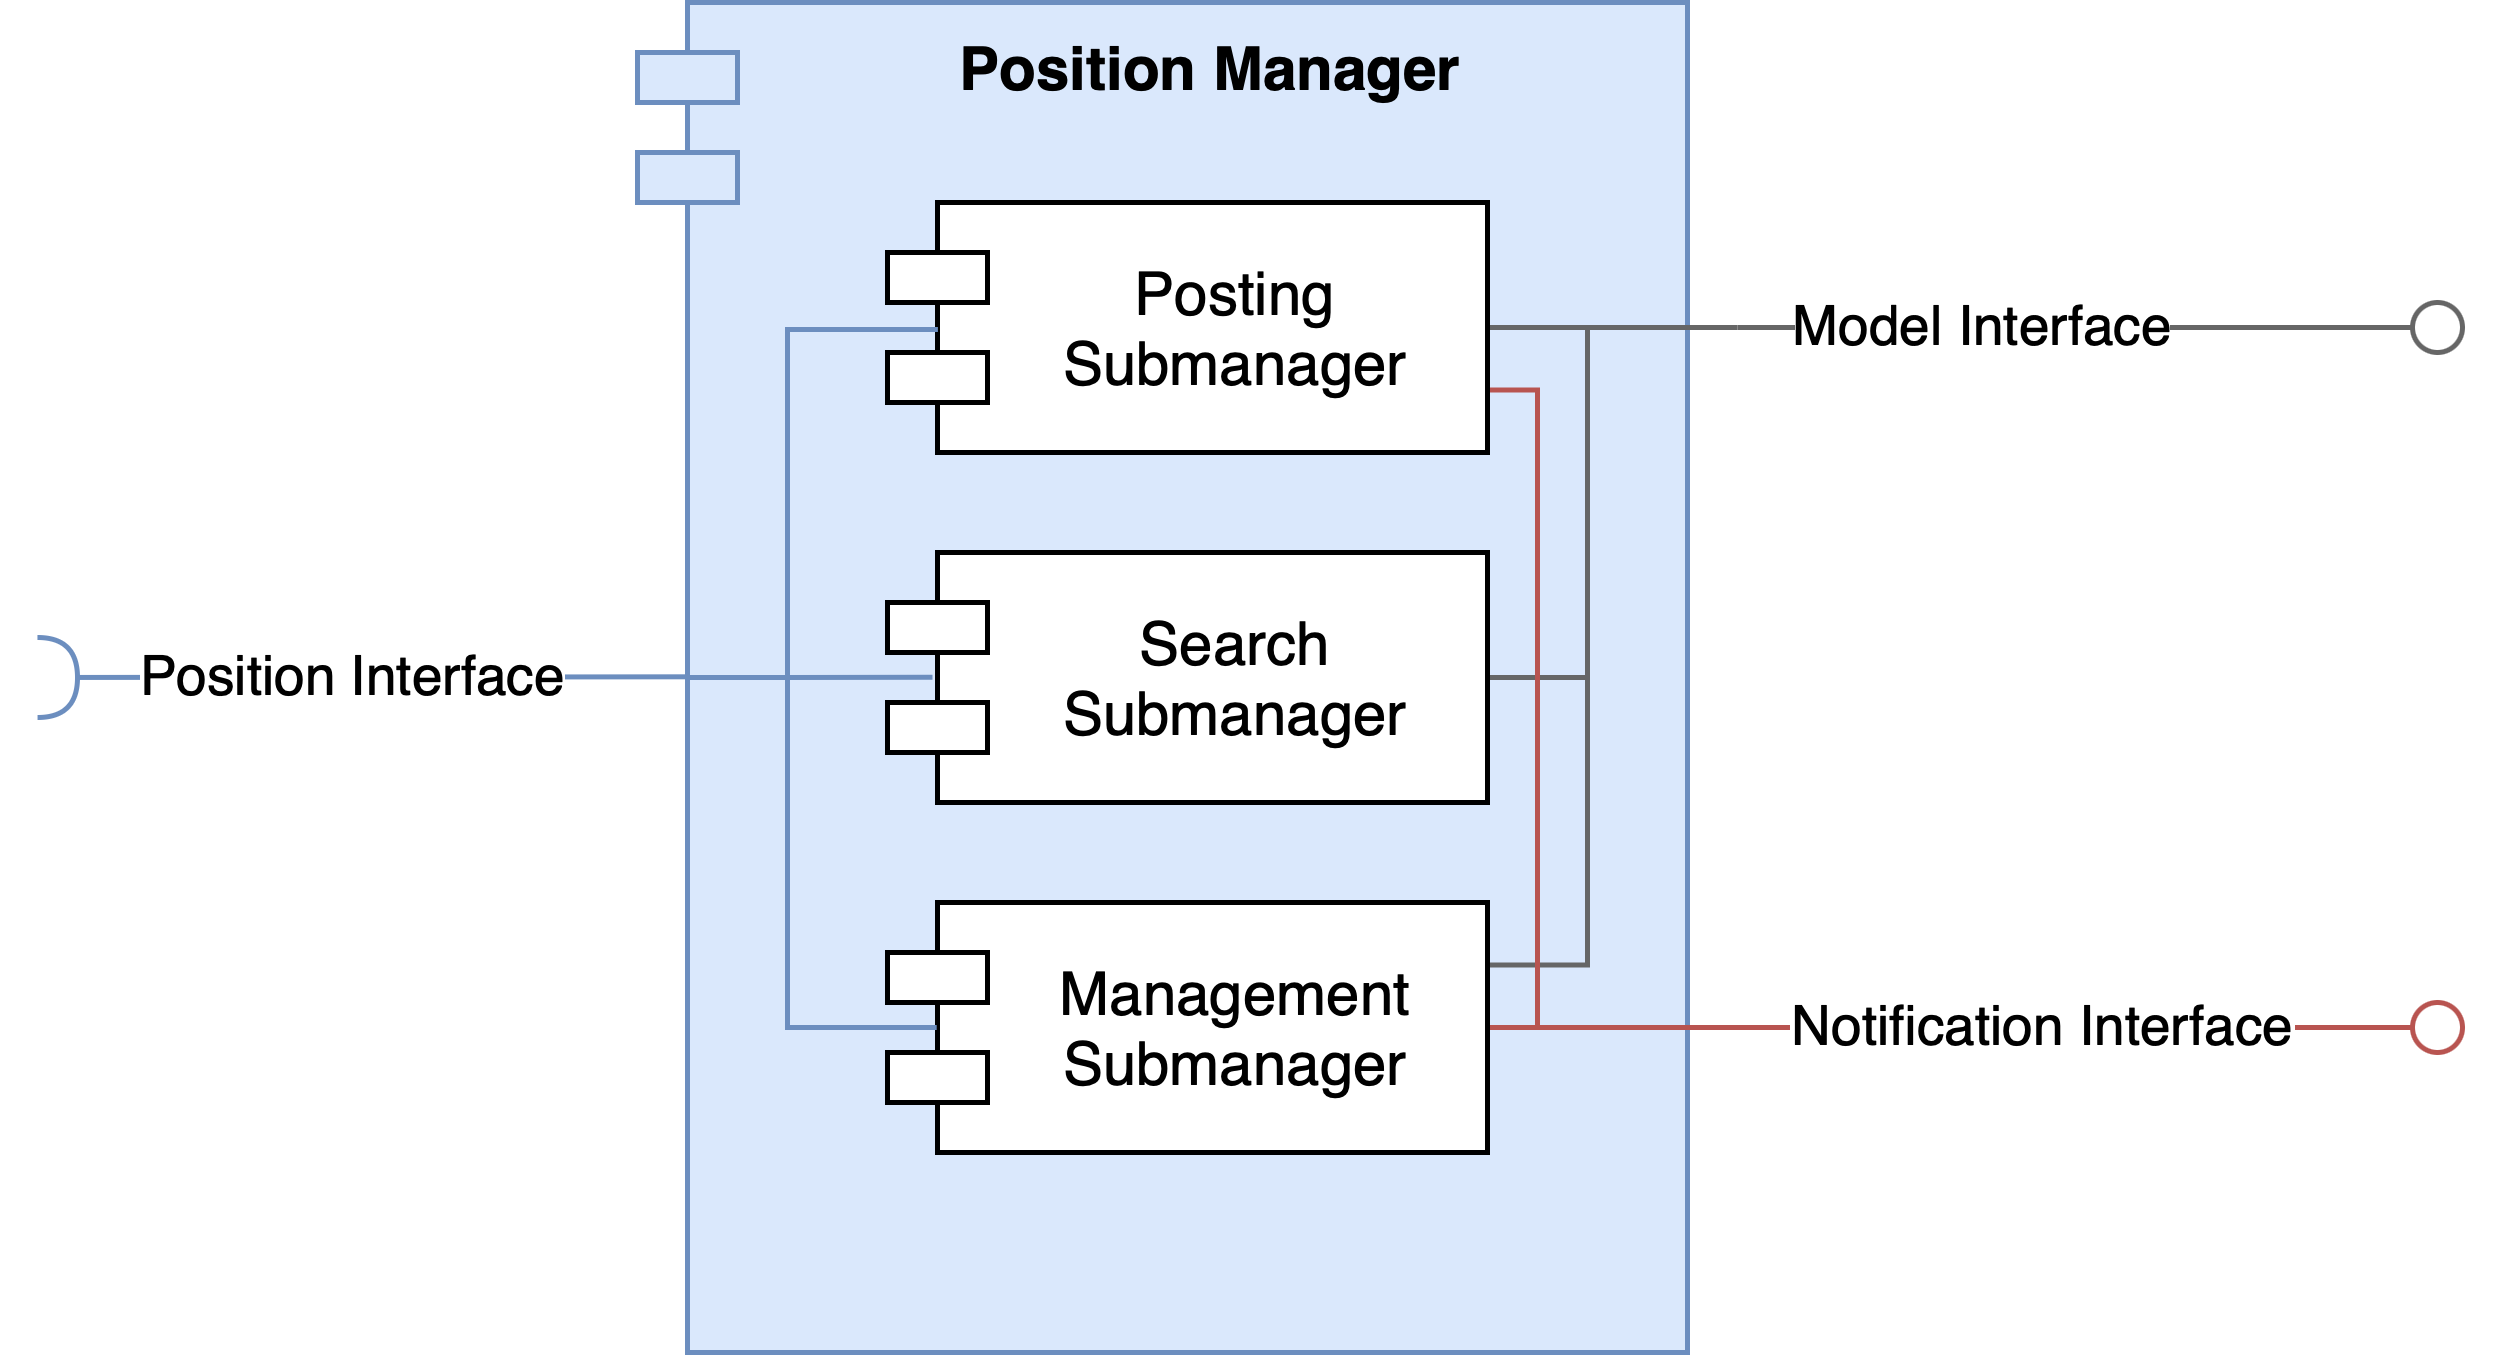
\includegraphics[width=11cm]{images/managers/position.png}
    \caption{Position manager}
\end{figure}

The position posting submanager allows companies to post new positions, validating details such as required skills and terms.

The position search submanager empowers students to search for opportunities through keywords.
It ranks and prioritizes results, highlighting the most relevant options.

The position management submanager supports companies in modifying existing position postings, ensuring all changes are logged, including updates in their status.

\subsubsection{Recommendation Manager}
The recommendation interface fuels the platform’s personalized experience by connecting users with tailored opportunities.
The recommendation manager transforms system data into actionable suggestions, enhancing engagement.

\begin{figure}[h]
    \centering
    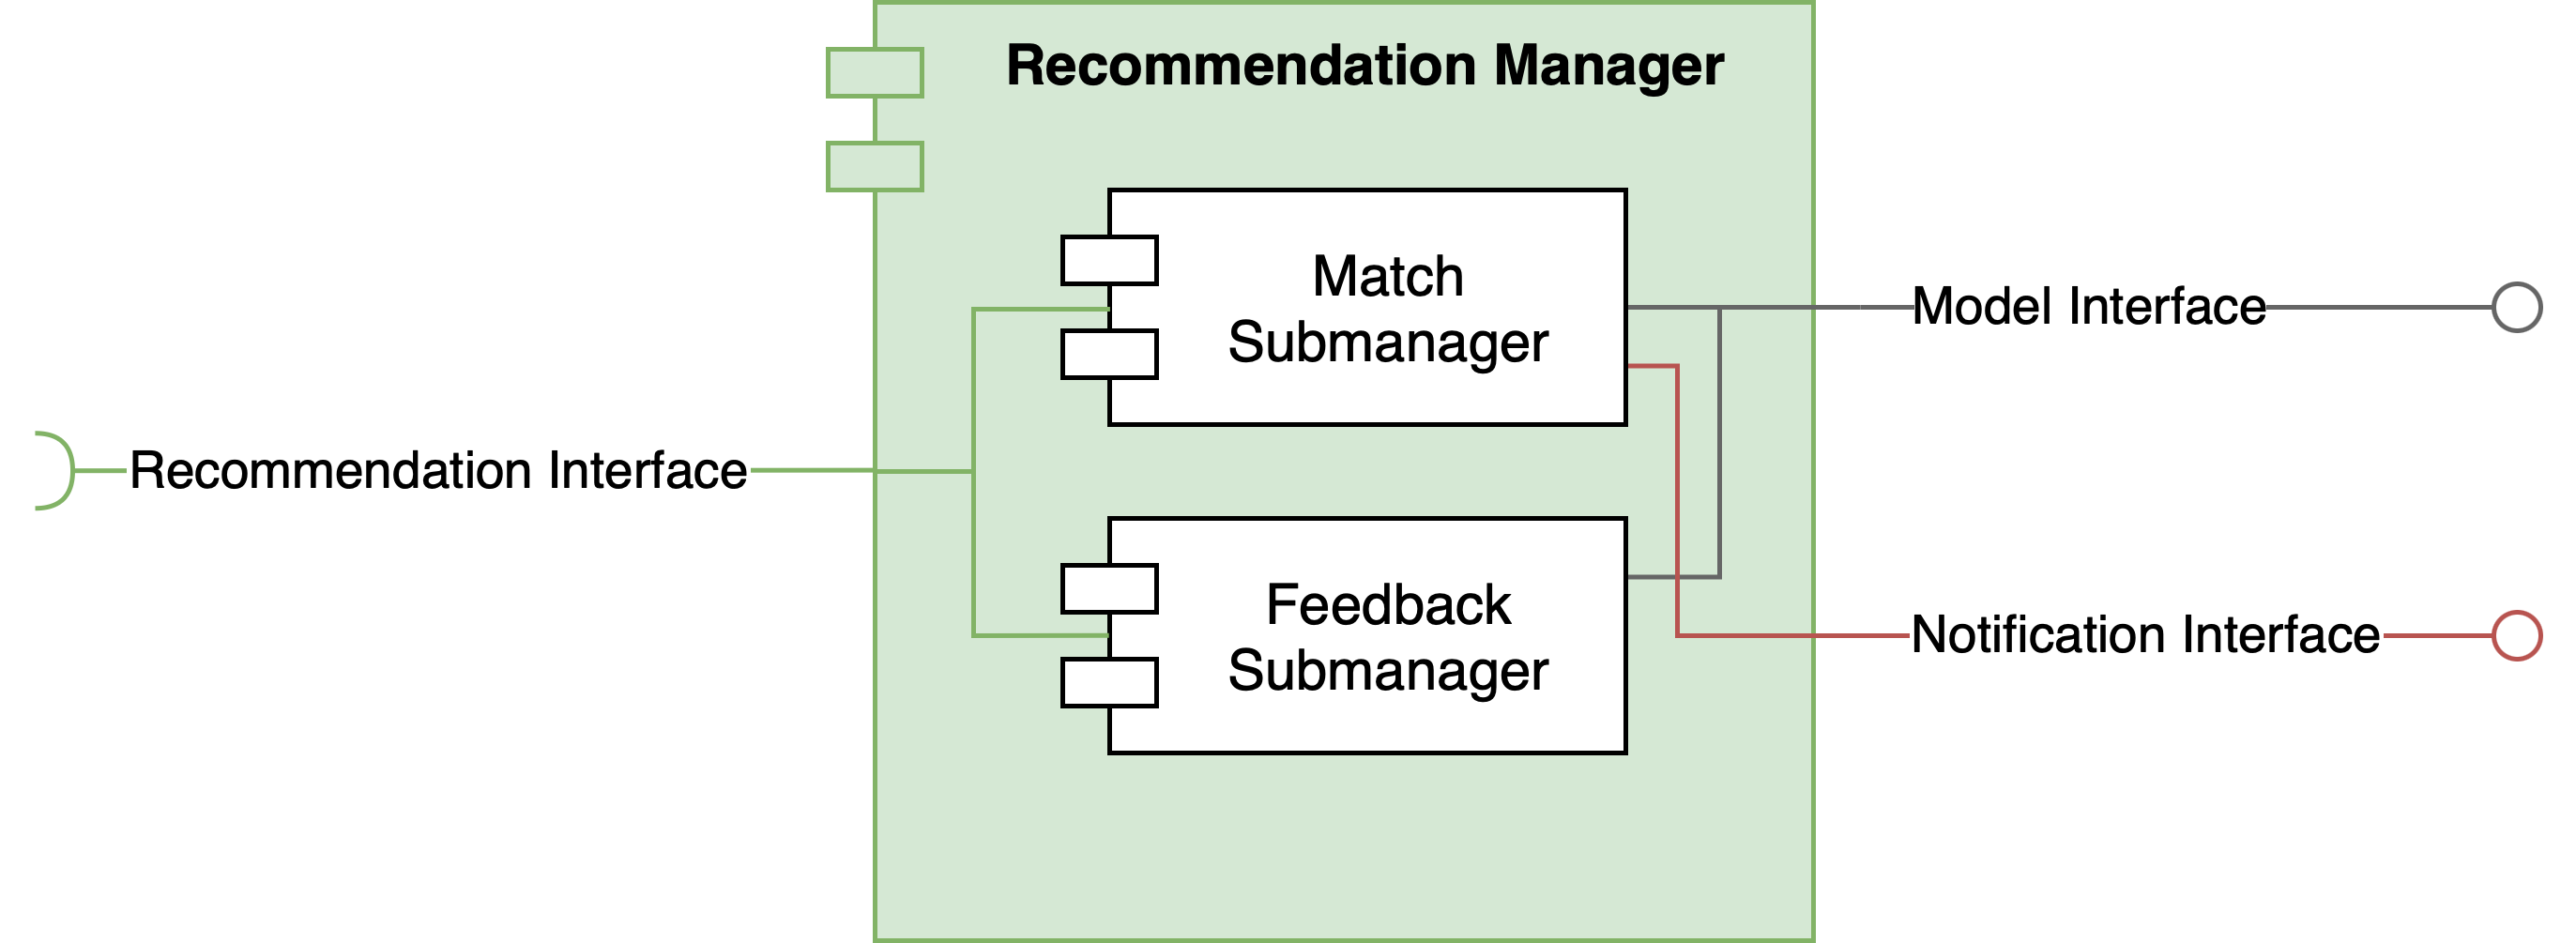
\includegraphics[width=12cm]{images/managers/recommendation.png}
    \caption{Recommendation manager}
\end{figure}

The recommendation match submanager applies statistical analysis to generate recommendations by comparing user profiles and position descriptions. It also ensures users are informed about new recommendations by working with the notification manager.

The recommendation feedback submanager tracks feedback forms to refine future suggestions, improving relevance over time.

\subsubsection{Selection Manager}
The selection interface connects university students and companies through the selection process, channeling application and interview workflows to the selection manager.

\begin{figure}[h]
    \centering
    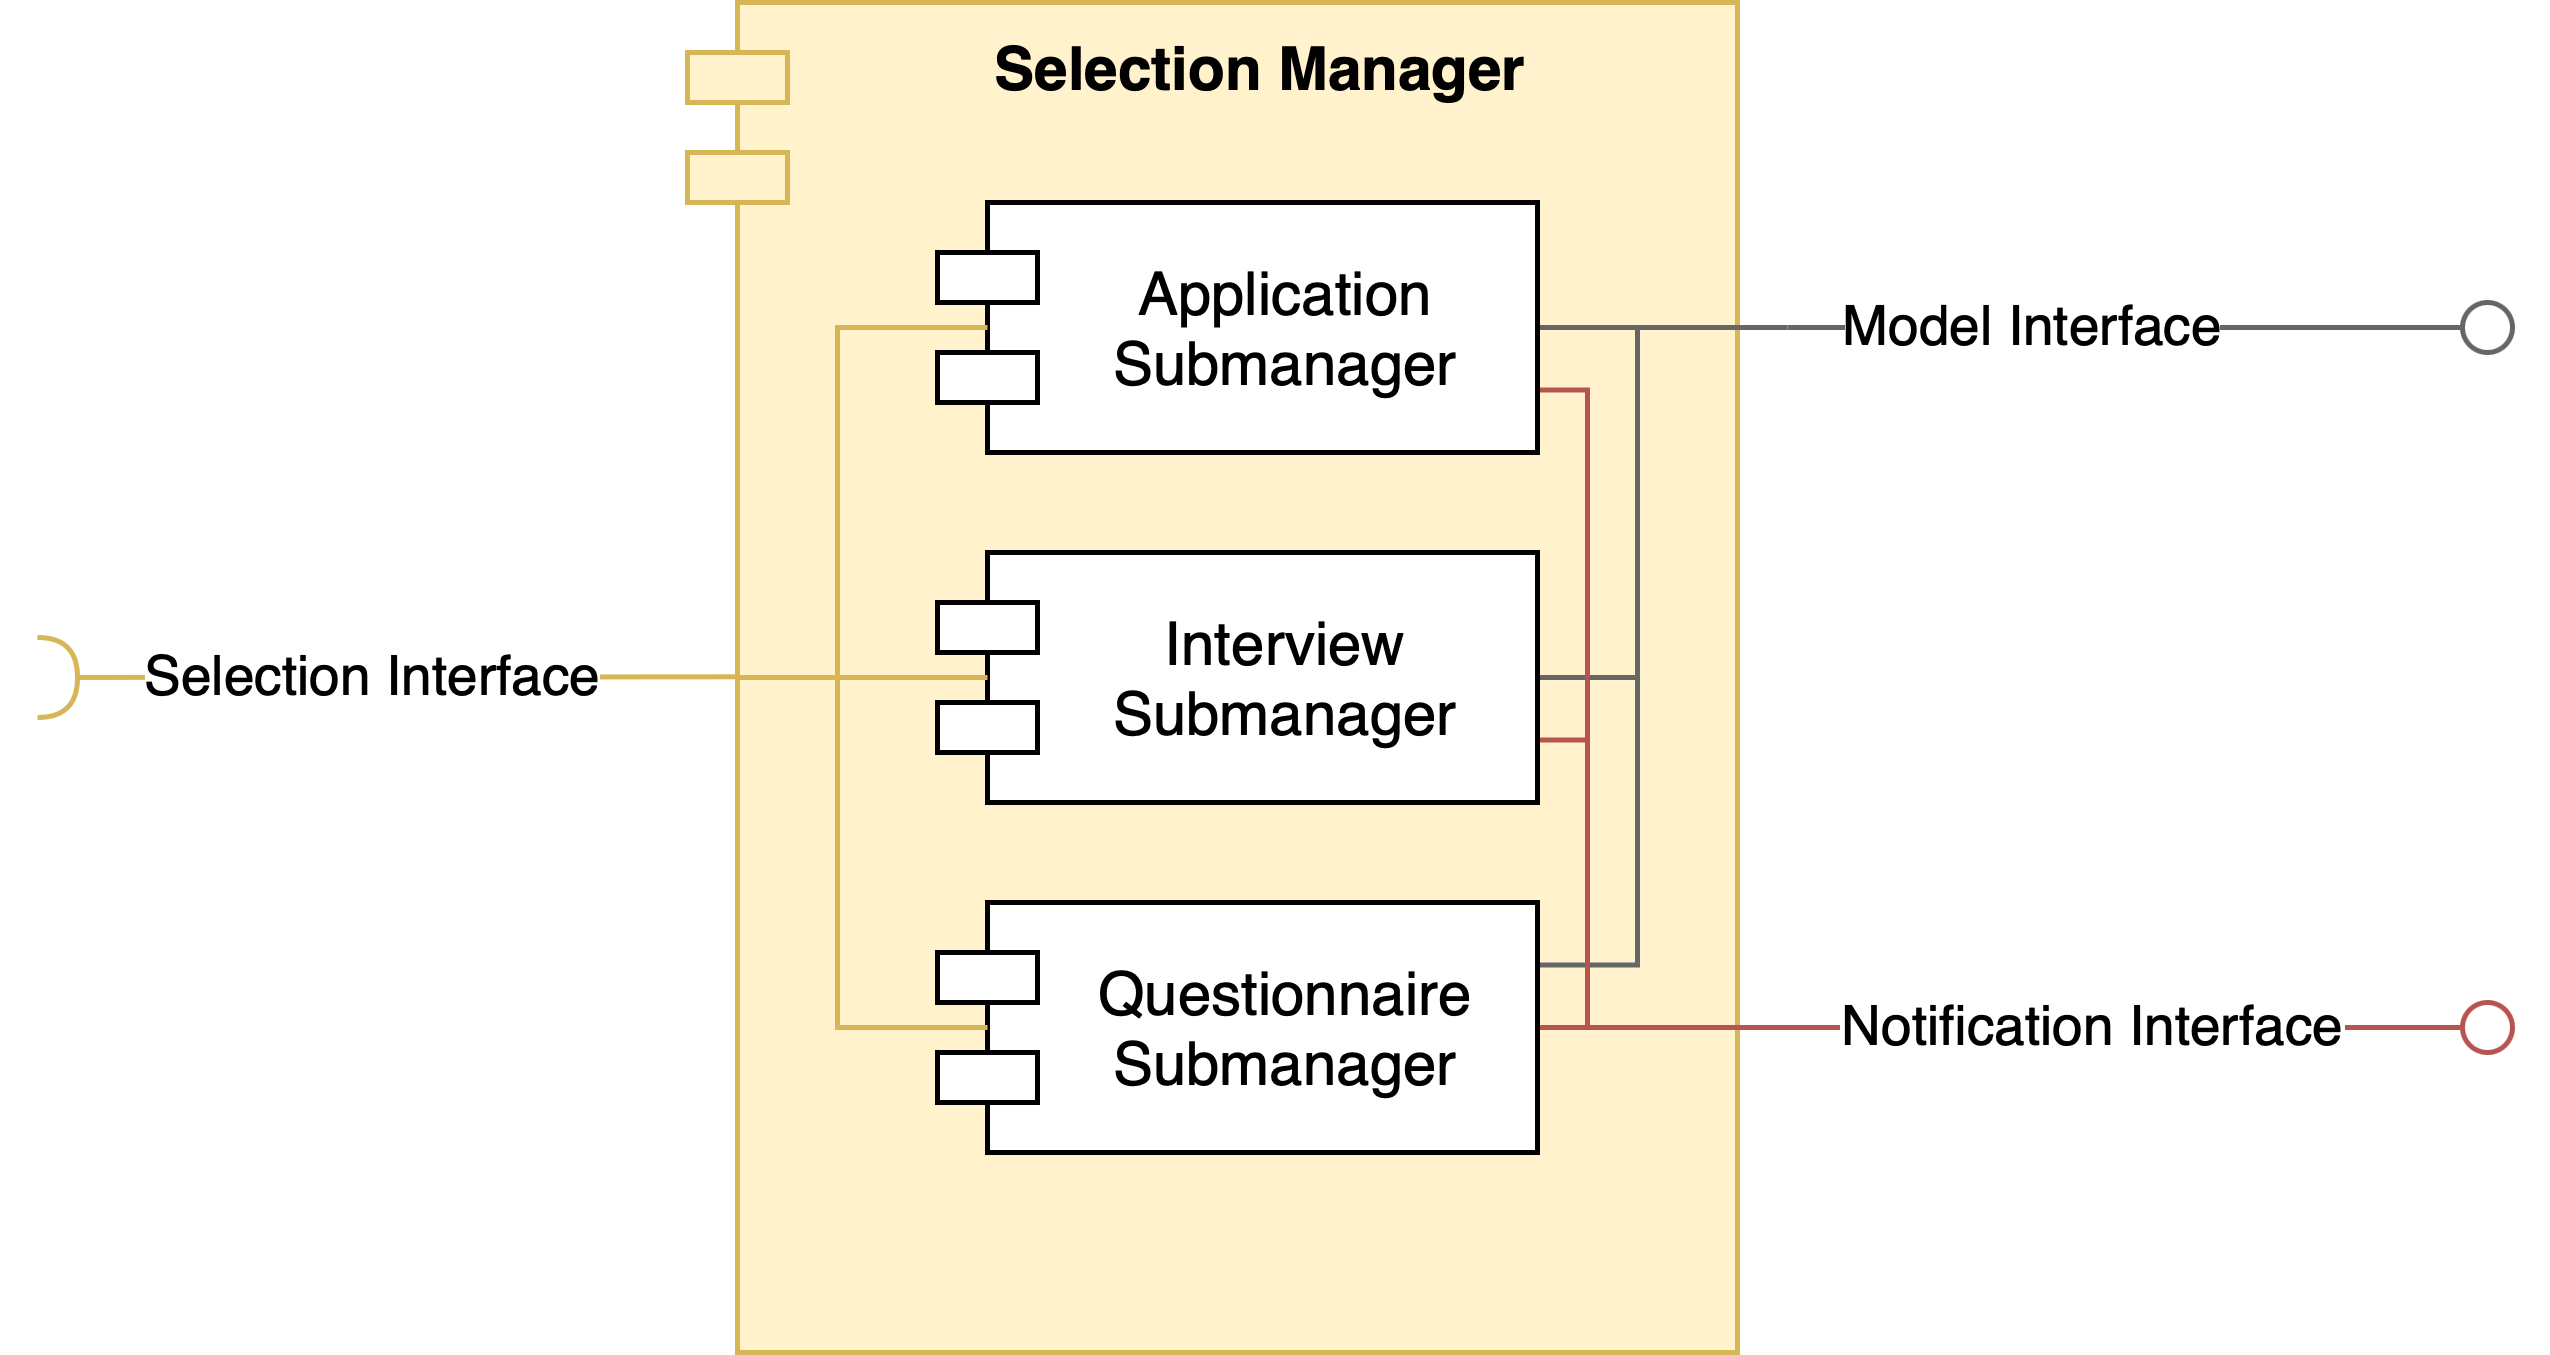
\includegraphics[width=11cm]{images/managers/selection.png}
    \caption{Selection manager}
\end{figure}

The selection application submanager oversees the lifecycle of applications, from initial submission to final outcome.
It makes sure that both students and companies are informed throughout the workflow by integrating with the notification manager.

The selection interview submanager coordinates interviews by validating availability and resolving conflicts, ensuring schedules are efficiently managed.

The selection questionnaire submanager supports companies in evaluating candidates by managing the distribution and storage of questionnaires.

\subsubsection{Internship Manager}
The internship interface facilitates collaboration among students, companies and universities, channeling related workflows to the internship manager.
This manager monitors ongoing internships, ensuring transparency.

\begin{figure}[h]
    \centering
    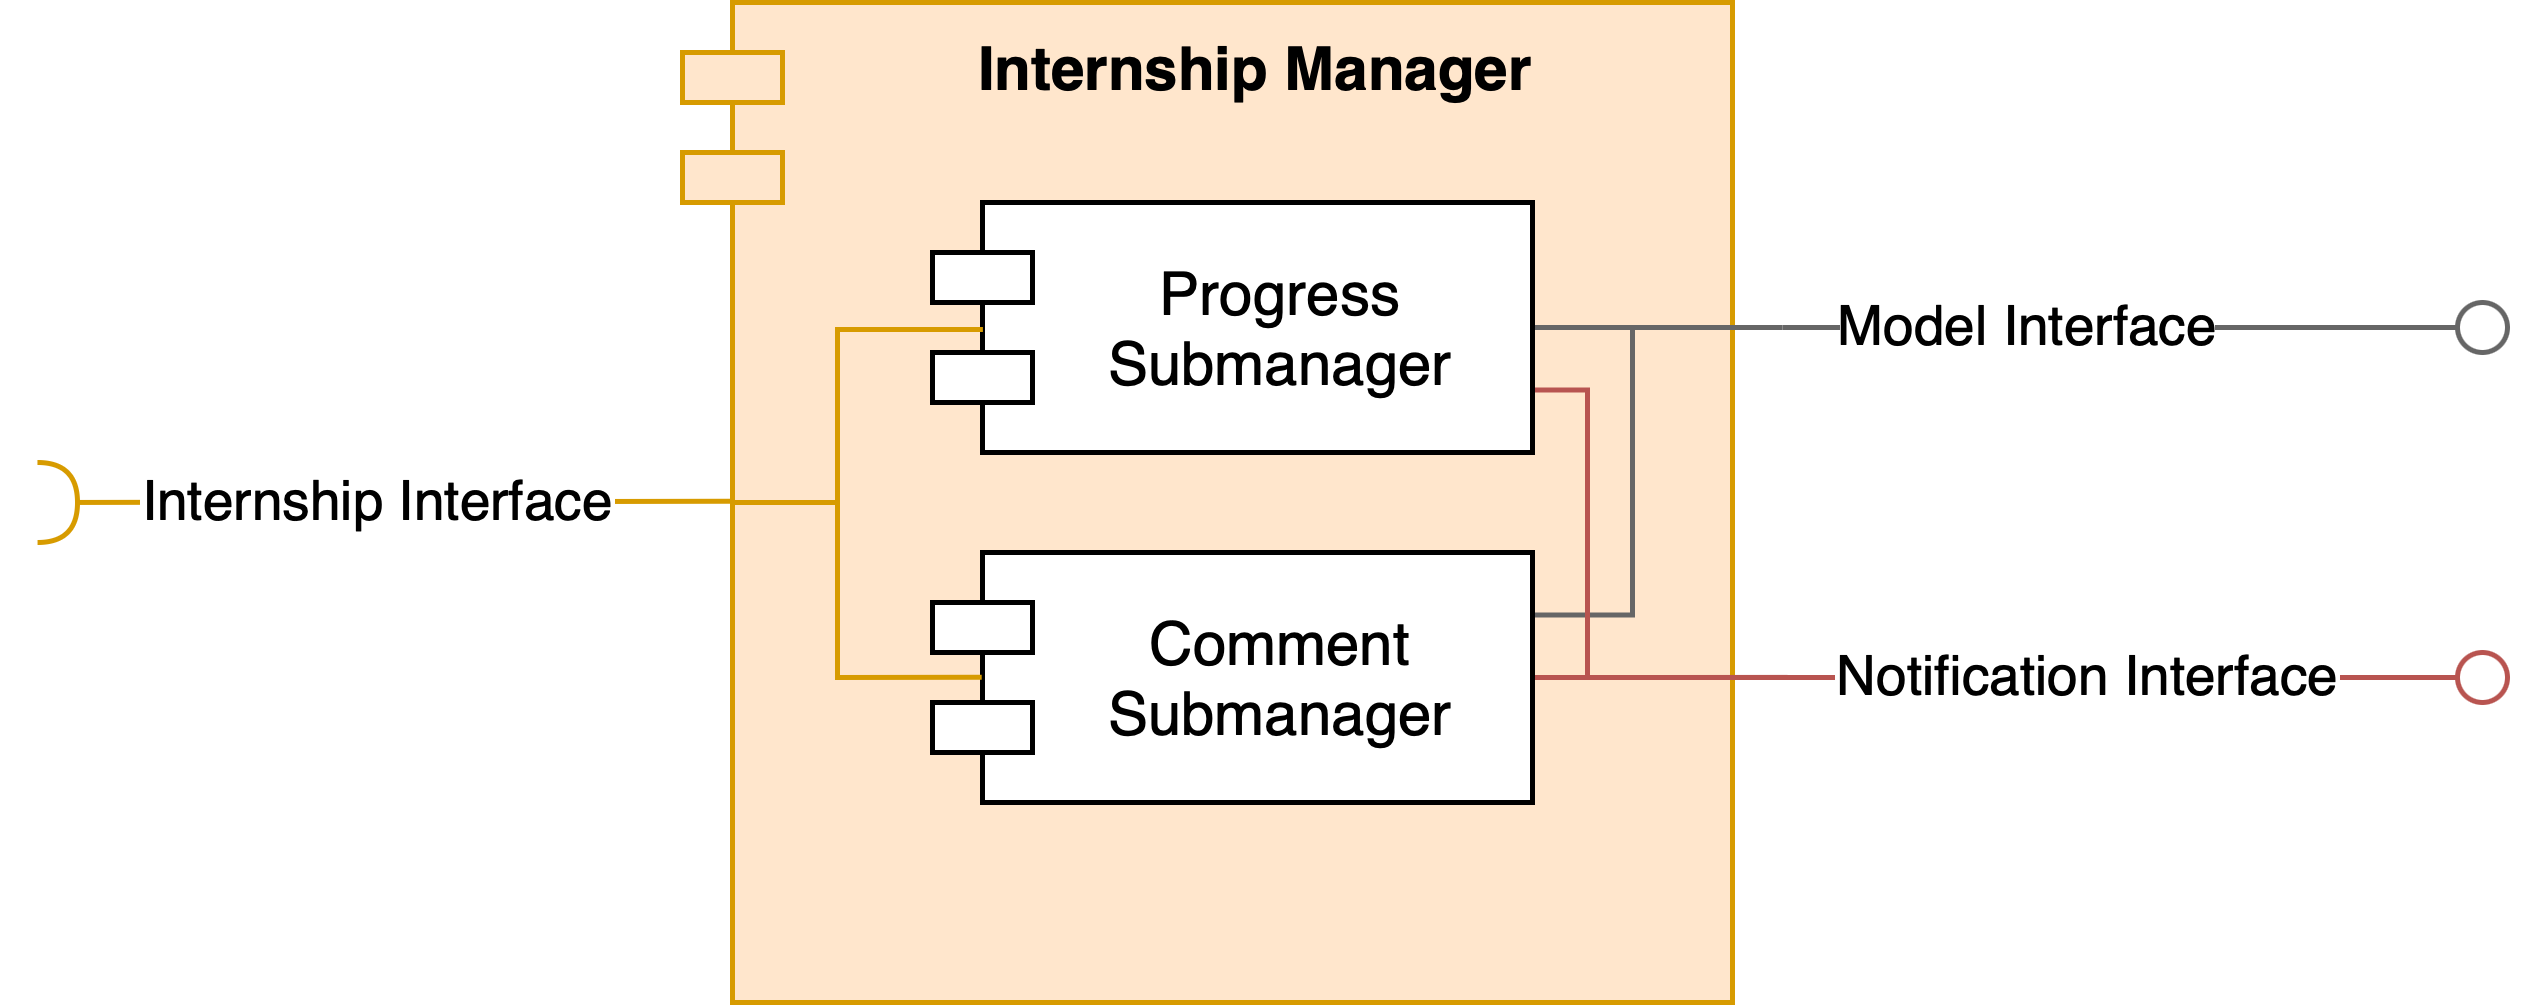
\includegraphics[width=11cm]{images/managers/internship.png}
    \caption{Internship manager}
\end{figure}

The internship progress submanager records status updates, providing all stakeholders with insights into internship progress.
Additionally, it collaborates with the notification manager to send update emails.

The internship comment submanager coordinates the posting of comments when progress is reported or a concern is raised.

\subsubsection{Notification Manager}
The notification interface connects other managers to the notification manager, which acts as the centralized hub for delivering all emails.
By consolidating communication, it ensures consistency and reliability across the system.

\begin{figure}[h]
    \centering
    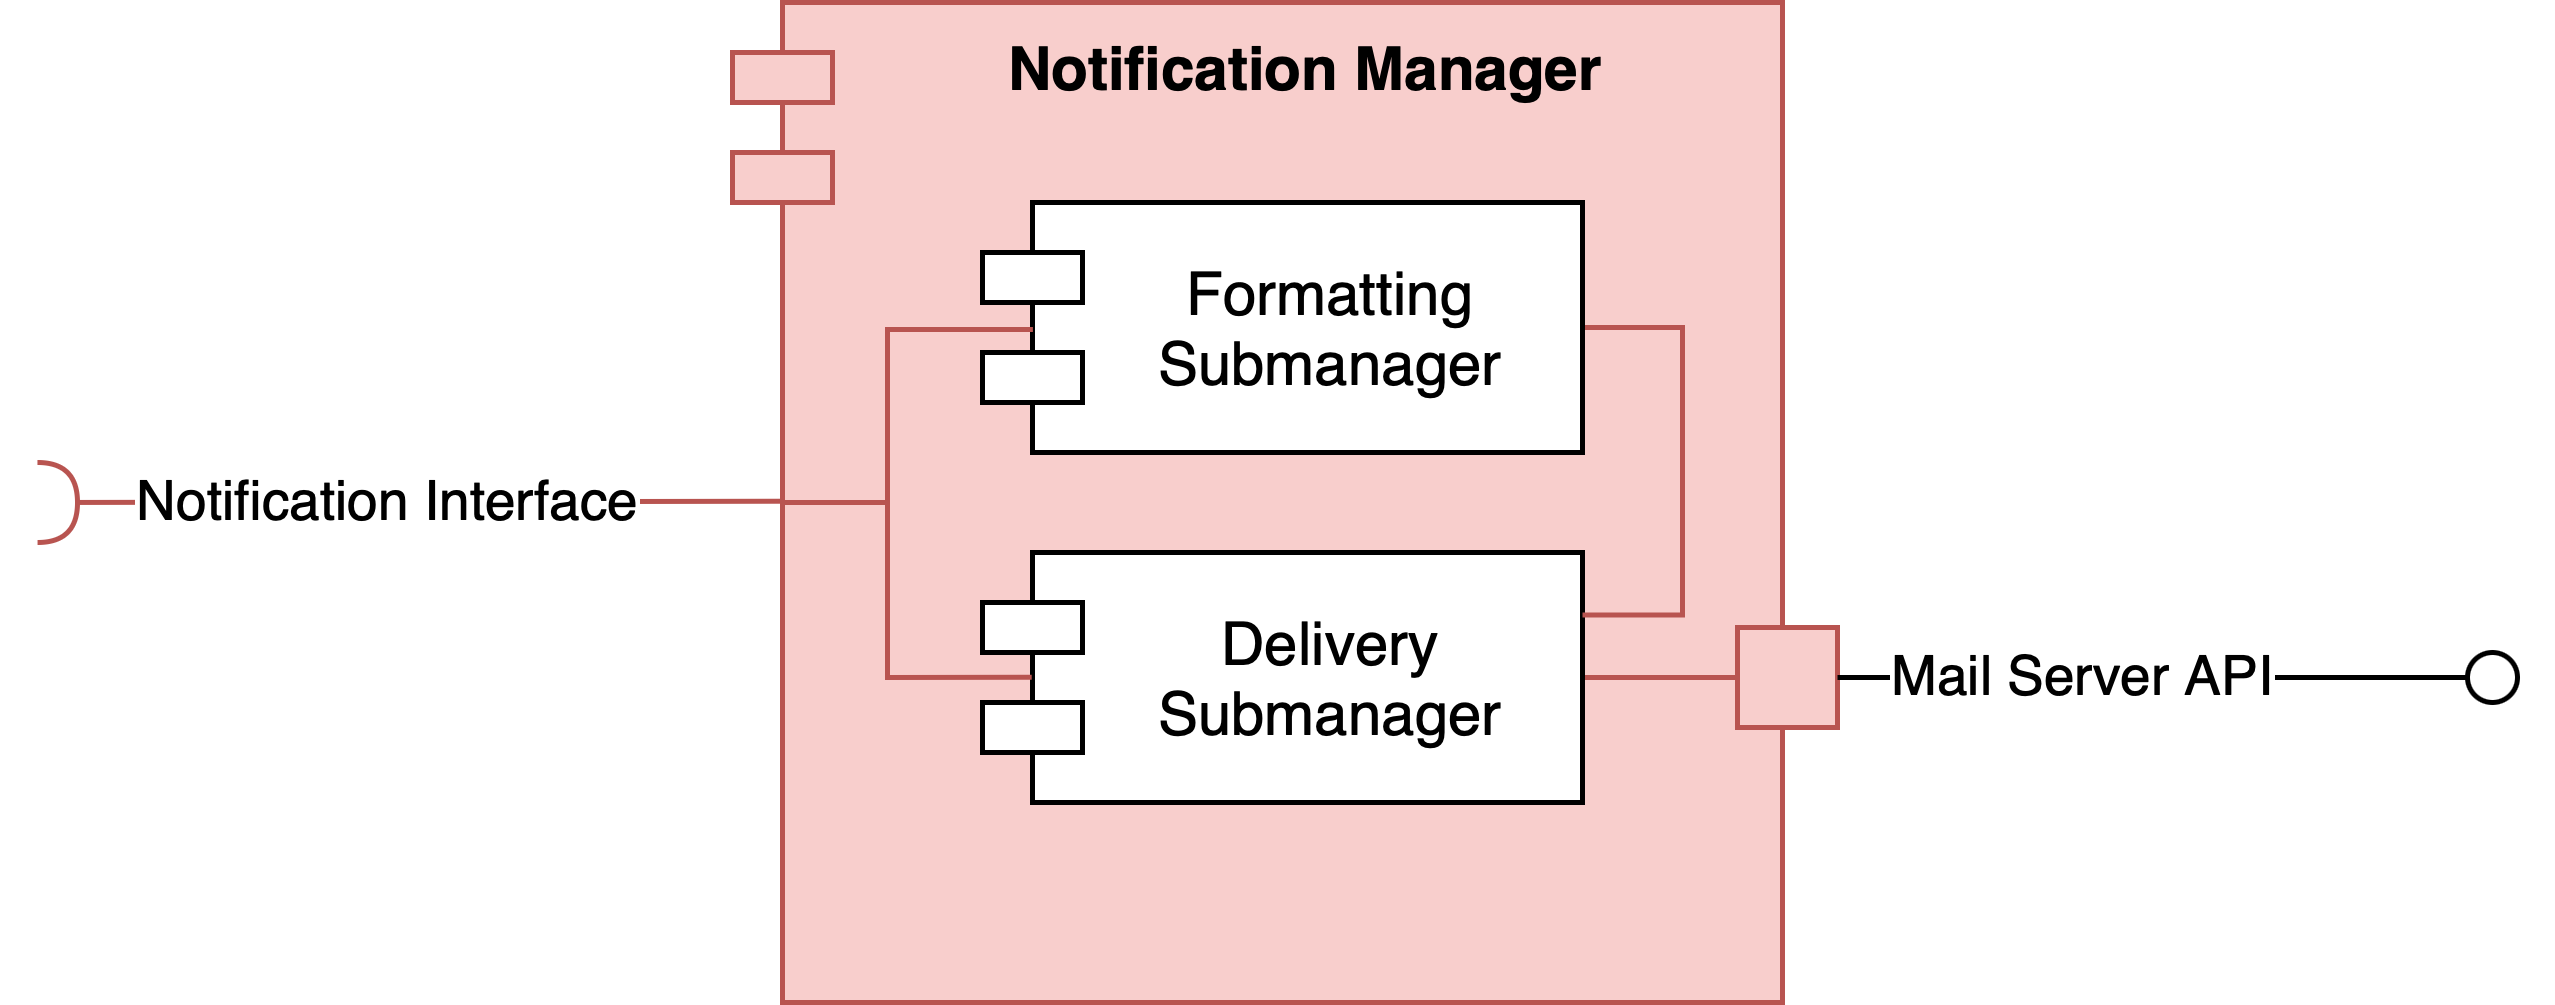
\includegraphics[width=11cm]{images/managers/notification.png}
    \caption{Notification manager}
\end{figure}

The notification formatting submanager prepares emails by structuring data provided by other managers, ensuring clarity for the recipient.

The notification delivery submanager communicates with the mail server API to send notifications, tracking delivery and retrying failed attempts to maintain reliability.

\section{Deployment View}
This section provides a detailed representation of how the software components are physically deployed on hardware nodes, together with their interactions.
It outlines the infrastructure, focusing on the communication protocols, security measures and data management strategies employed in the system.
The deployment is designed to align with the three-tier architecture defined in the overview:

\begin{figure}[h]
    \centering
    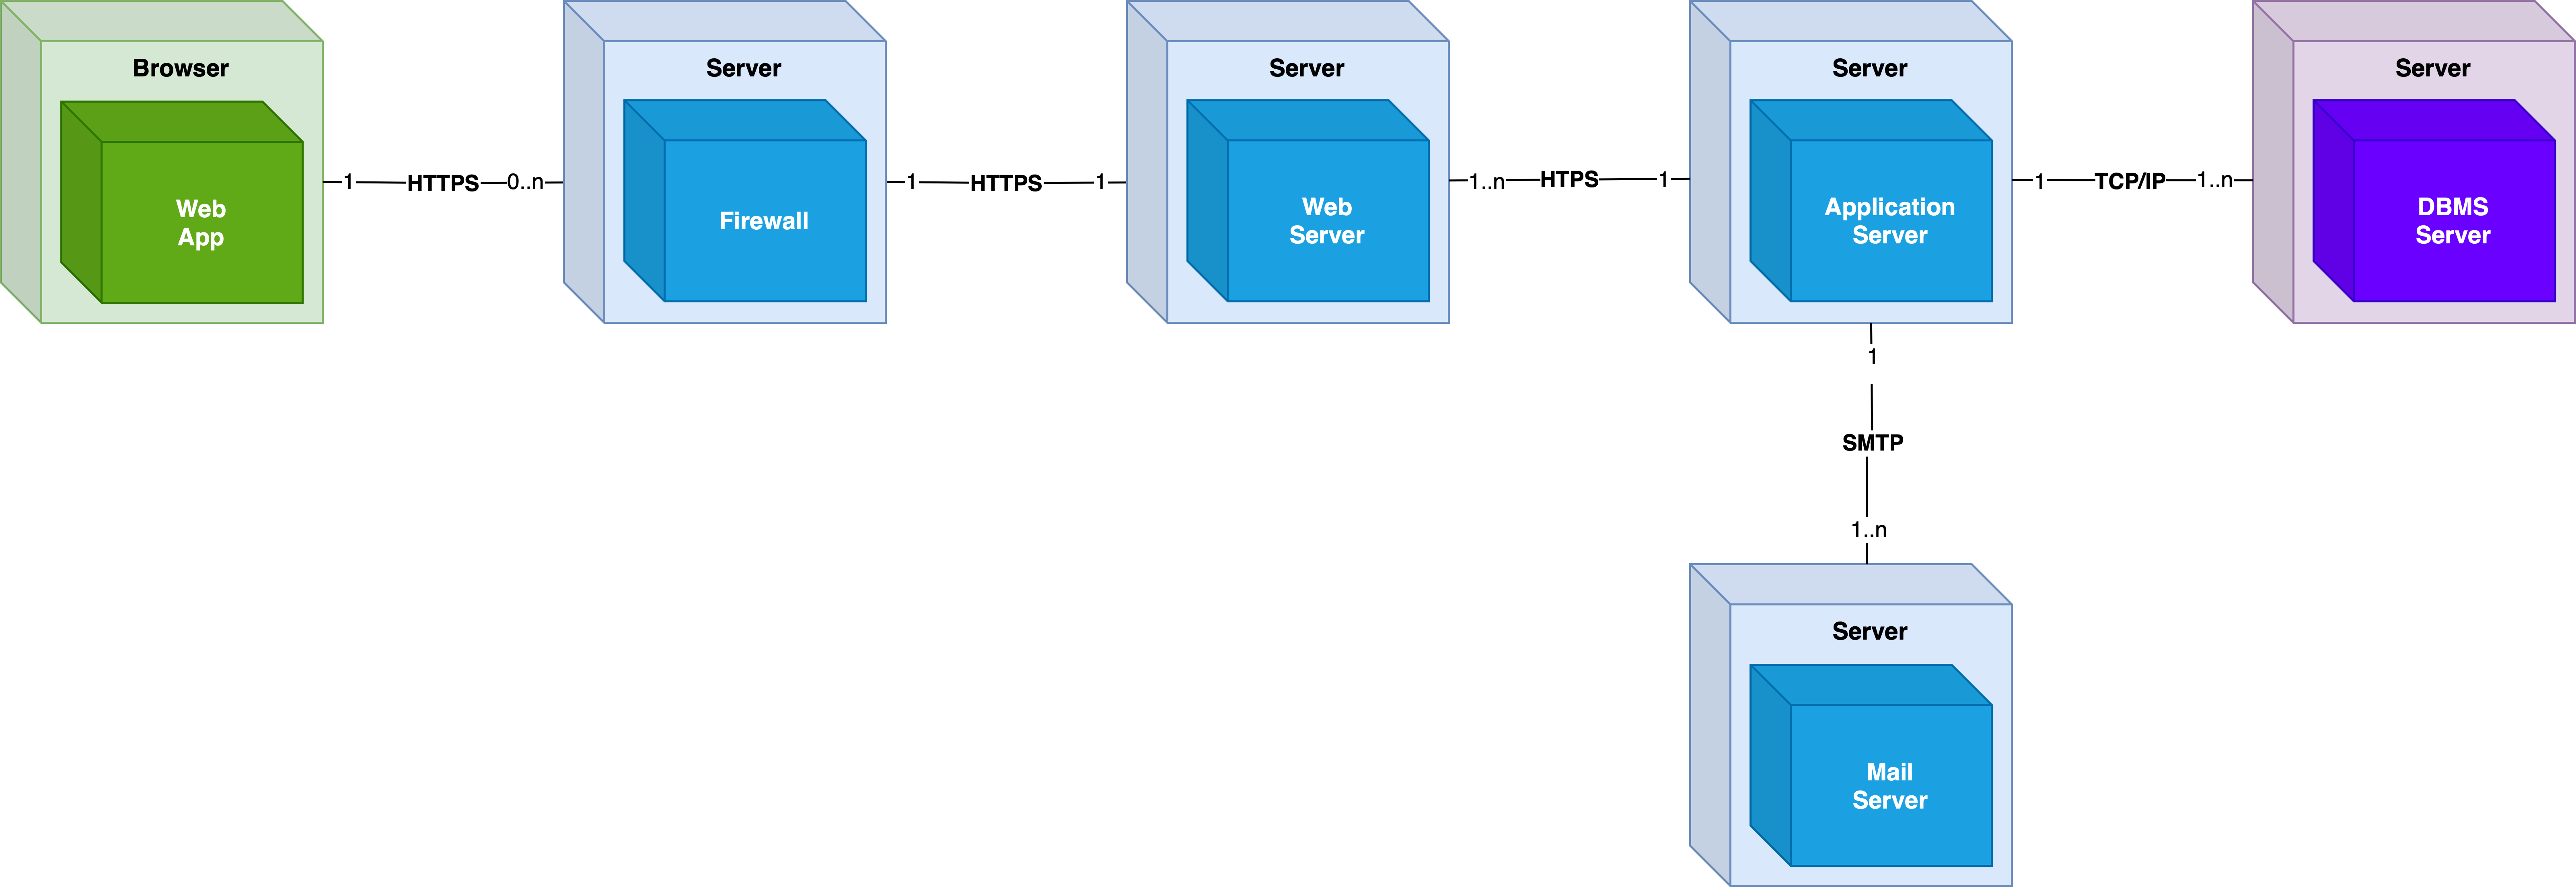
\includegraphics[width=16cm]{images/deployment-view.png}
    \caption{Deployment view}
\end{figure}

A firewall is deployed between the browser and the web server to protect the internal infrastructure.
It acts as the first line of defense by filtering incoming traffic and allowing only HTTPS requests on designated ports.
This ensures that exclusively legitimate traffic reaches the web server, mitigating risks of unauthorized access or malicious attacks.

The connection between the browser and the web server, and subsequently between the web server and the application server, uses HTTPS.
This protocol encrypts all transmitted data, ensuring confidentiality and integrity for securing sensitive operations such as user authentication.
The application server then communicates with the DBMS server using the TCP/IP protocol, providing reliable and ordered data exchange.
This is suitable for database queries and responses, ensuring accurate transactions between the application and the database.
Lastly, the application server interacts with the mail server to send emails using SMTP.
This ensures efficient email delivery while separating email-related tasks from core application processes.

A relational database management system such as PostgreSQL is used for structured data storage.
This aligns with the need for a well-defined schema and ACID compliance.
On ther other hand, files such as uploaded CVs are stored locally on the DBMS server’s file system.
Rather than storing the binary data in the database itself, the file paths are saved as references in it.
This approach separates structured data from unstructured data, optimizing database performance and simplifying file management.

\section{Runtime View}
\section{Component Interfaces}
\section{Architectural Styles and Patterns}
This section examines the architectural styles adopted in Students\&Companies, explaining their general principles and how they guide implementation decisions.
Understanding these foundational patterns is crucial for developers working on the system, as they influence everything from component interaction to code organization.

\subsubsection{Client-Server Architecture}
The system's foundation rests on a client-server architecture, which separates systems into service requesters, called clients, and service providers, called servers.
This separation enables the user interface to evolve independently from data processing and storage, while centralizing resource management on the server.
Developers can thus focus on their domain, either crafting responsive user experiences or implementing robust business logic.

Modern applications refine this pattern through tiers, which are logical groupings of related functionality.
A three-tier architecture divides the application into three distinct layers: a presentation tier that handles the user interface, an application tier that processes business logic and a data tier that manages storage.
This separation gives developers clear boundaries for their work and lets teams works independently, reducing development bottlenecks and simplifying maintenance.

\subsubsection{REST Architecture}
REST (Representational State Transfer) guides how these tiers communicate over the web.
Originally conceived for document transfer, REST has evolved into a comprehensive style for data exchange.
Its core principle of statelessness means that servers maintain no information about past requests.
Instead, each client request must contain all necessary context.
This architectural choice significantly impacts development: backend developers need not manage complex session states, system administrators benefit from straightforward load balancing since any server can handle any request and cache developers can optimize performance by focusing solely on request parameters rather than server state.

\subsubsection{MVC Pattern}
The Model-View-Controller (MVC) pattern organizes software into three interconnected components, each with distinct responsibilities.
The model represents the core data structure, encapsulating the database, while the view handles user interaction and presentation.
Controllers act as intermediaries, processing user requests to run business logic and coordinate workflows.
This separation of concerns enhances scalability, modularity and maintainability, allowing developers to focus on specific aspects of the system without impacting others, ultimately fostering efficient collaboration among teams.

\section{Other Design Decisions}
While architectural styles and patterns provide the system's foundation, many other critical design decisions shape its implementation.
This section outlines these choices, focusing on practical aspects that developers must consider when implementing the system.

\subsubsection{Deployment Approach}
The deployment strategy embraces horizontal scaling, running multiple application server instances rather than scaling up individual servers.
This approach requires developers to write stateless code that works across instances, but provides significant benefits: the system continues functioning even if some instances fail, resource allocation becomes more flexible as administrators can add or remove instances based on demand and load balancing becomes straightforward since any instance can handle any request.

\subsubsection{Security Implementation}
Security permeates every aspect of the design through multiple complementary layers: all client-server communication uses HTTPS encryption to protect data in transit, sensitive information receives additional encryption in the database and session management relies on time-limited tokens rather than storing session data server-side.

\subsubsection{Data Management}
Data management emphasizes both integrity and performance: the database implements transaction management to maintain consistency even during concurrent operations, constraint enforcement catches validity issues early and performance optimization through strategic indexing and caching improves response times.


\chapter{User Interface Design}
This chapter presents the user interface design of Students\&Companies, focusing on its structure and functionality to cater to students, companies and universities.
The objective of the design is to create a seamless, intuitive and efficient user experience.
To achieve this, it adheres to core principles that enhance simplicity, accessibility and consistency throughout the platform.

Ensuring consistency across the system, the design employs uniform fonts, colors and layouts, allowing users to navigate with ease and confidence.
Accessibility is a key tenet, with the interface accommodating users with disabilities and ensuring responsiveness across devices by adhering to Web Content Accessibility Guidelines (WCAG).
Finally, simplicity drives the design process, prioritizing logical workflows that minimize user effort and facilitate task completion.

\section{Flow Diagram}
The flow diagram below serves as a map of the platform's pages, illustrating their interconnections.
It provides a unified view to highlight overlaps and parallelisms across the functionalities for students, companies and universities.
This approach underscores the distinct aspects of the navigation while emphasizing its coherence.

\begin{figure}[h]
    \centering
    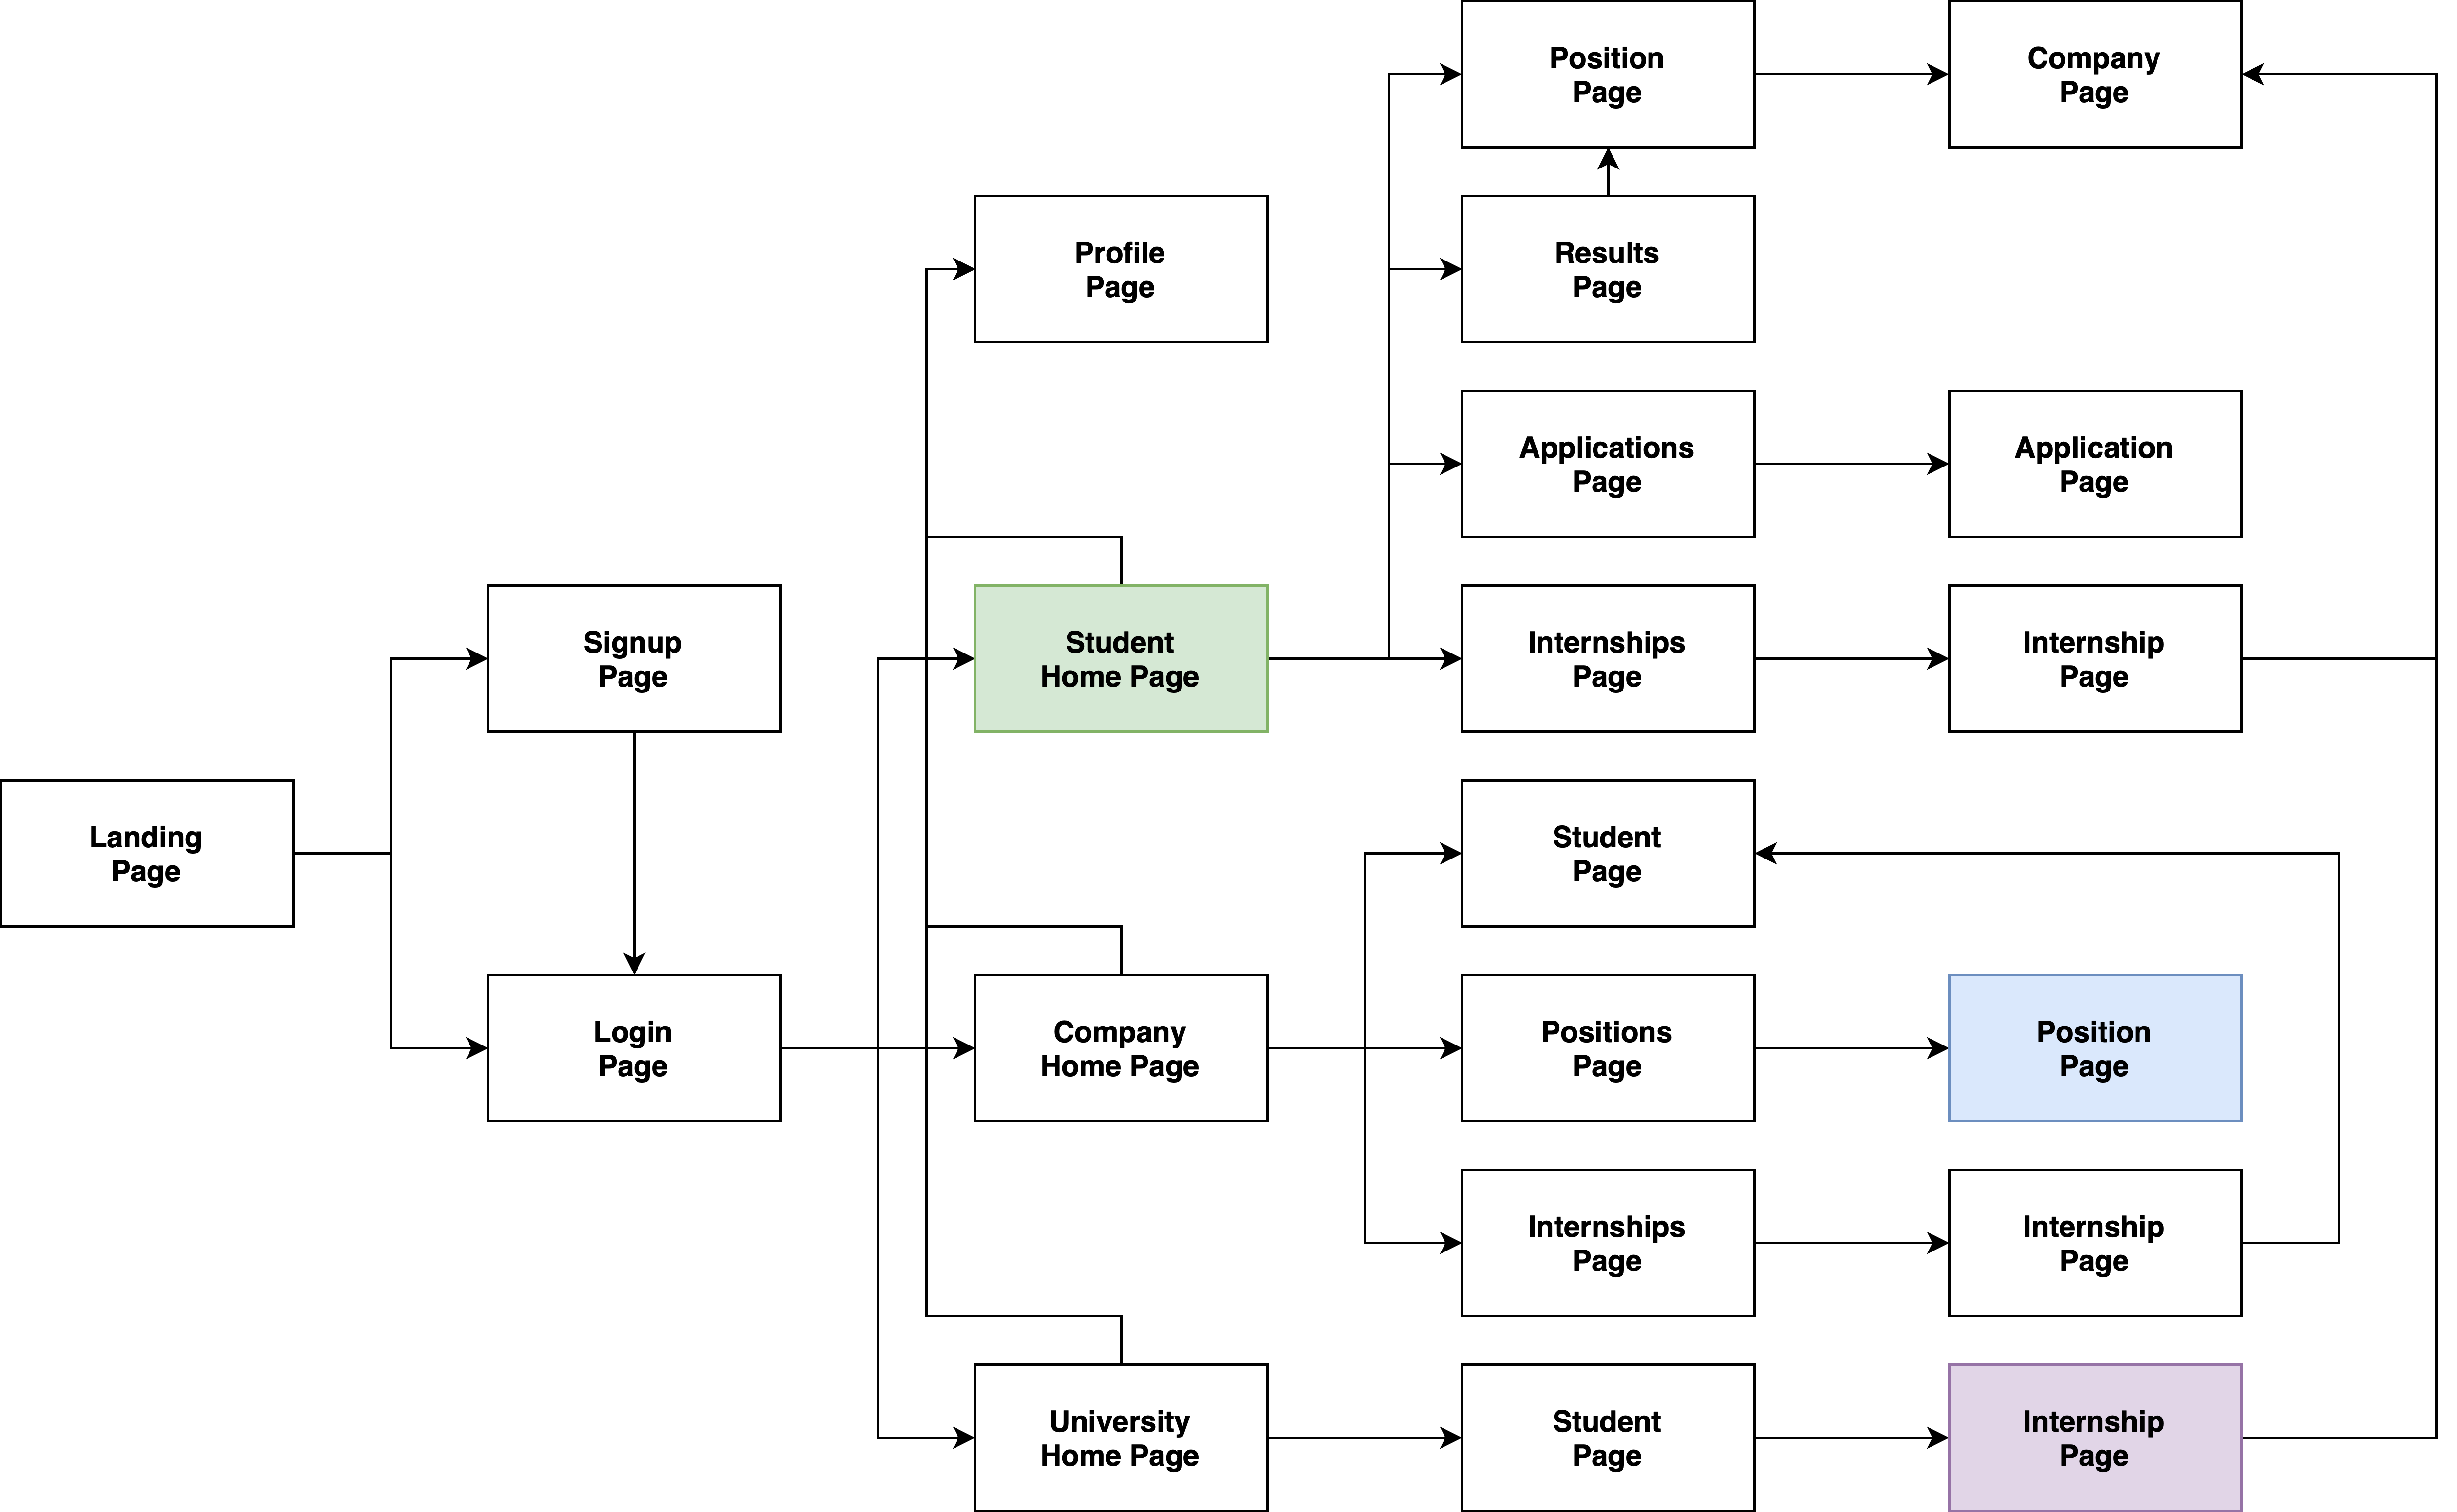
\includegraphics[width=16cm]{images/flow-diagram.png}
    \caption{Flow diagram}
\end{figure}

All primary pages of the platform are represented in this diagram, providing an overview of the core user workflows.
To maintain clarity, some finer details, such as the profile and questionnaire editors, interview page, feedback and comment forms, have been omitted but are mentioned in the requirements analysis and specification document \cite{carraracurrodossi2024}.
The pages highlighted in the diagram will be discussed in detail in the next section as they have been chosen as representative examples that showcase both the functionalities and the needs of each user category.

\section{Selected Pages}
The following section focuses on a selection of key pages within the platform.

\newpage
\subsection{Student Homepage}
The student homepage serves as the central hub for university students, designed to help them discover and apply for internship positions.
It features a header that includes links to the pages outlined in the flow diagram: the home, applications, internships and profile pages.
Note that this header is consistent across all of these pages, ensuring seamless navigation.
Similarly, the footer contains standard links such as privacy policy, terms of service and contact information, maintaining uniformity throughout the platform.

The main body of the homepage is focused on enabling students to search and explore positions.
It includes a search bar with filters for location, job type and field, allowing users to refine their results.
Below it, a list of recommendations is displayed.
Each position includes essential details such as location, job type and field, with options to expand for more information.
Students can view an expanded description of the position, along with clear buttons to either accept or reject the recommendation.

\begin{figure}
    \centering
    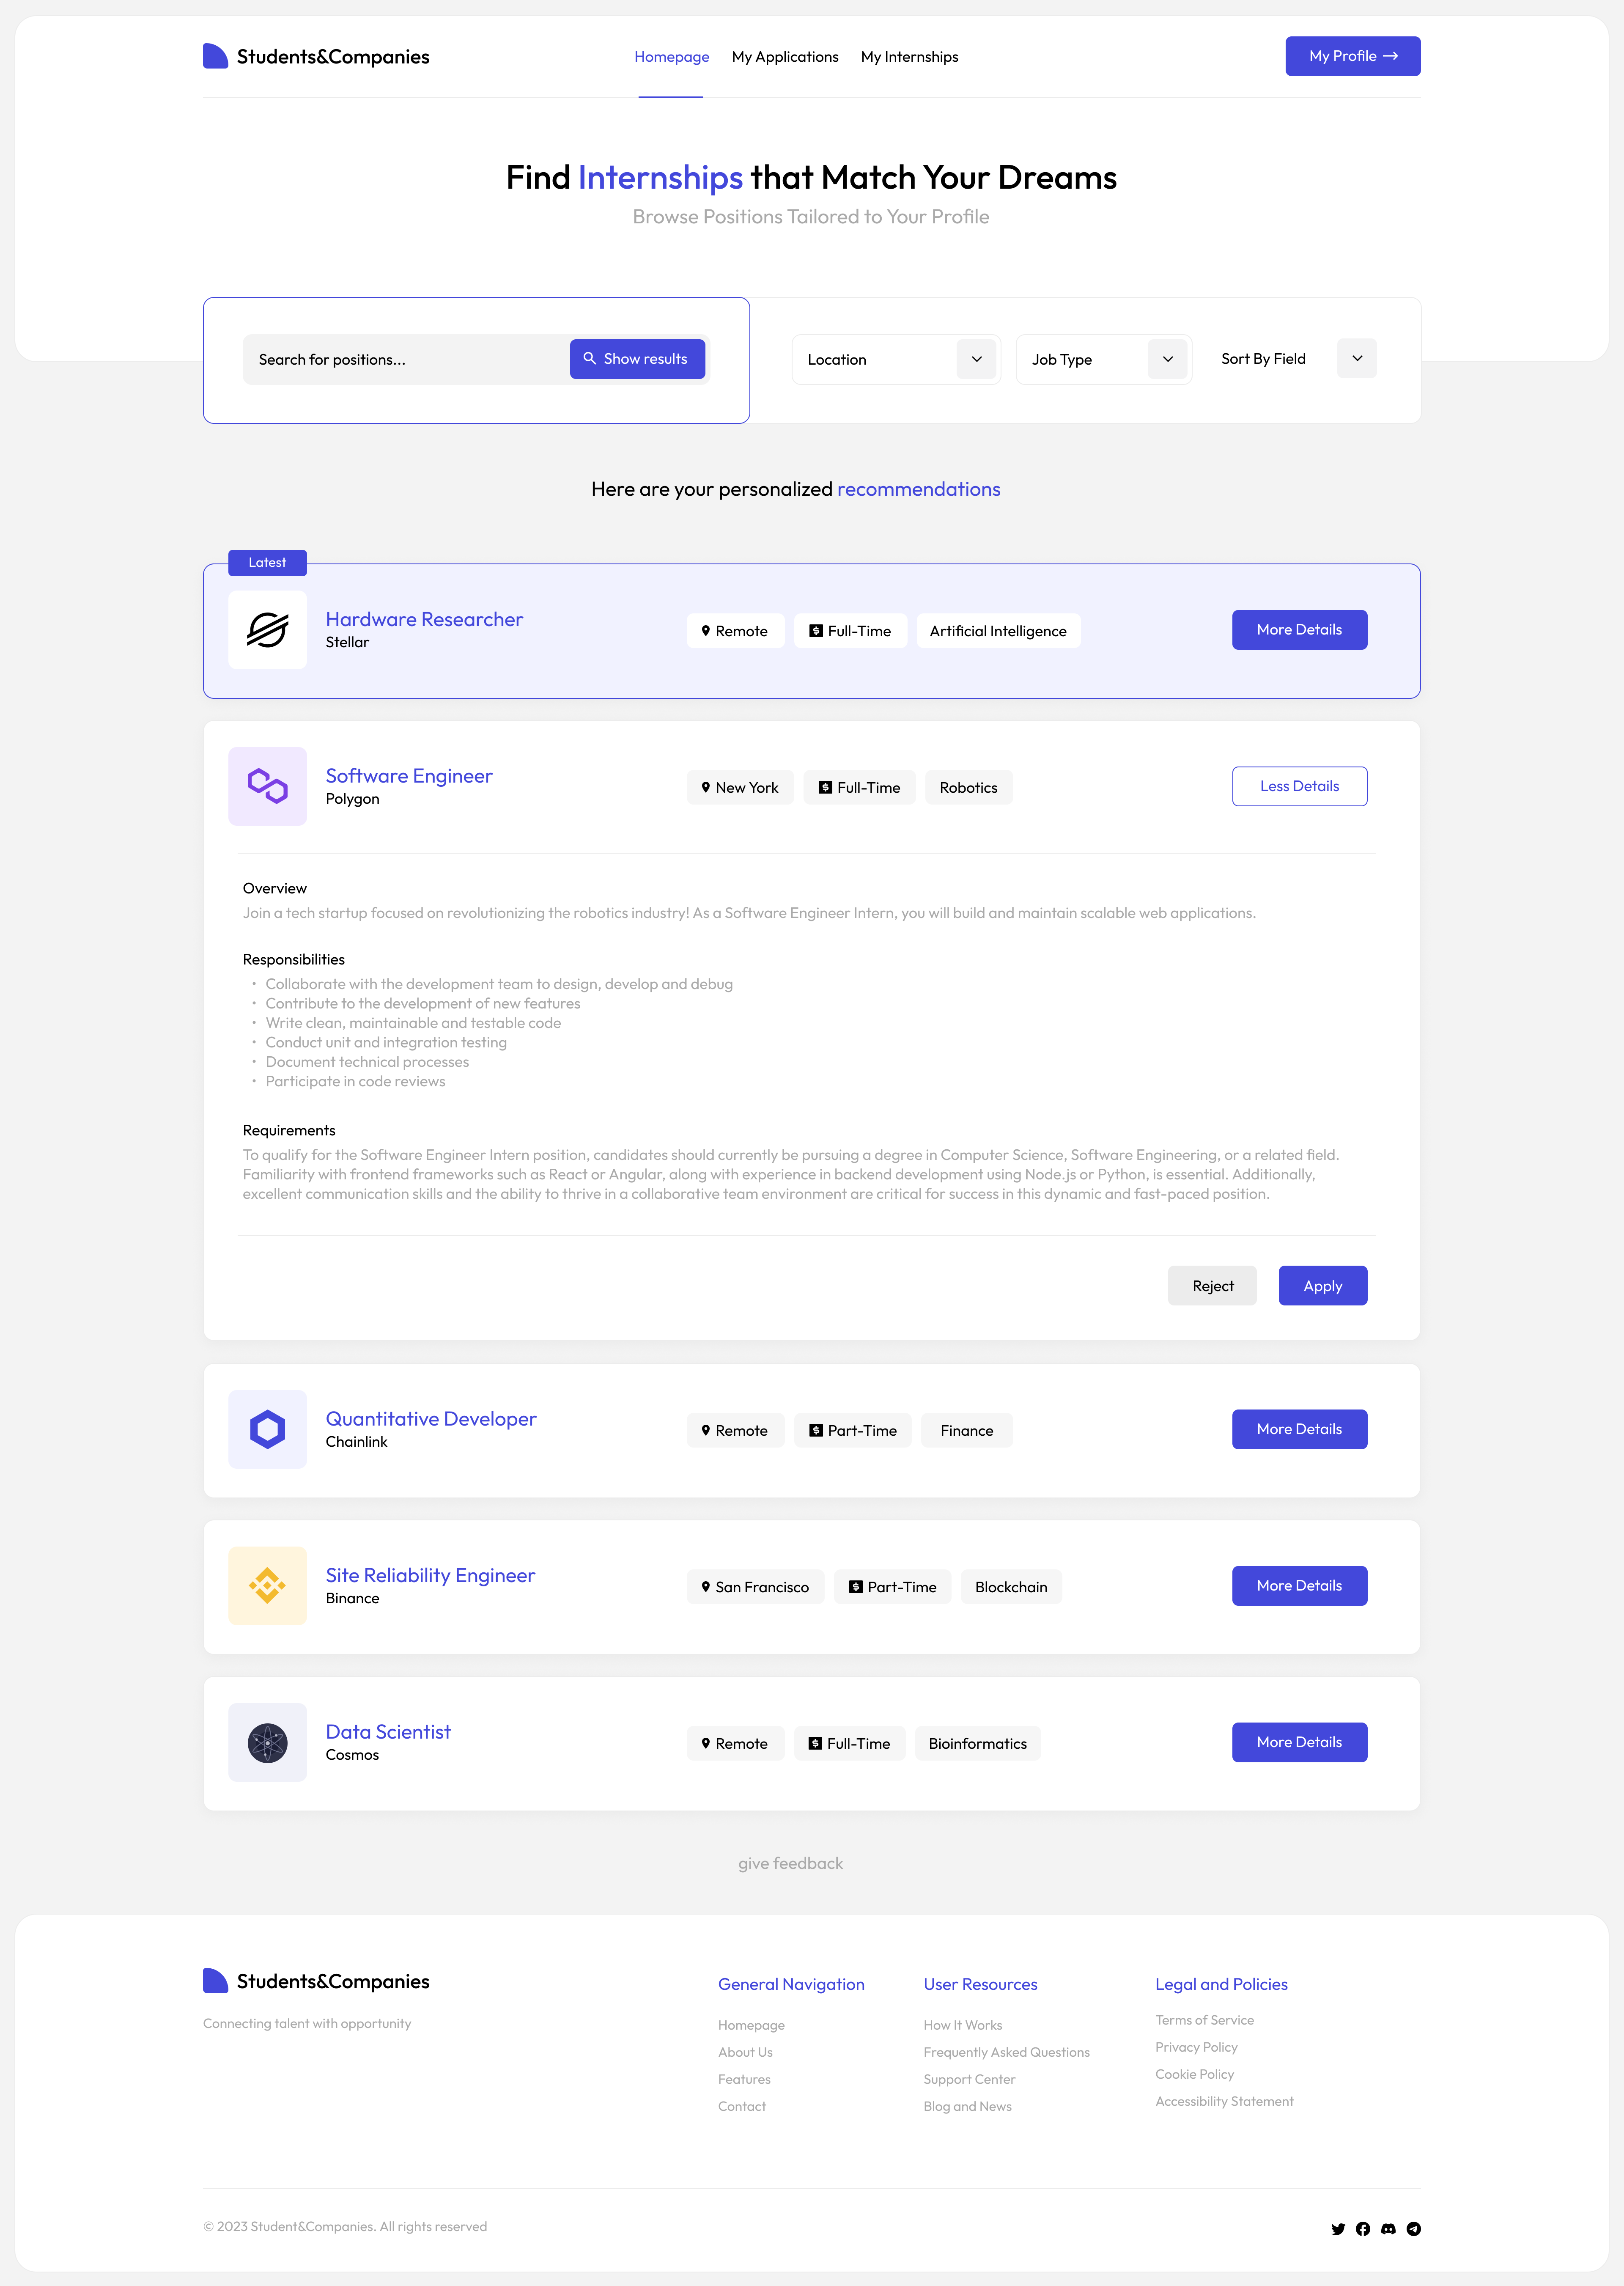
\includegraphics[width=15cm]{images/selected-pages/student-homepage.png}
    \caption{Student homepage}
\end{figure}

\subsection{Company Position Page}
The company position page maintains consistency with the platform's design through a familiar header and footer.
The body contains buttons for adding a questionnaire and scheduling an interview, with the date and time of the upcoming interview prominently displayed.
Below, it lists the questionnaires filled out by the student, which can be expanded to review answers.
Based on his performance, the company can either select or reject the candidate using the respective buttons, streamlining the selection process.

\begin{figure}
    \centering
    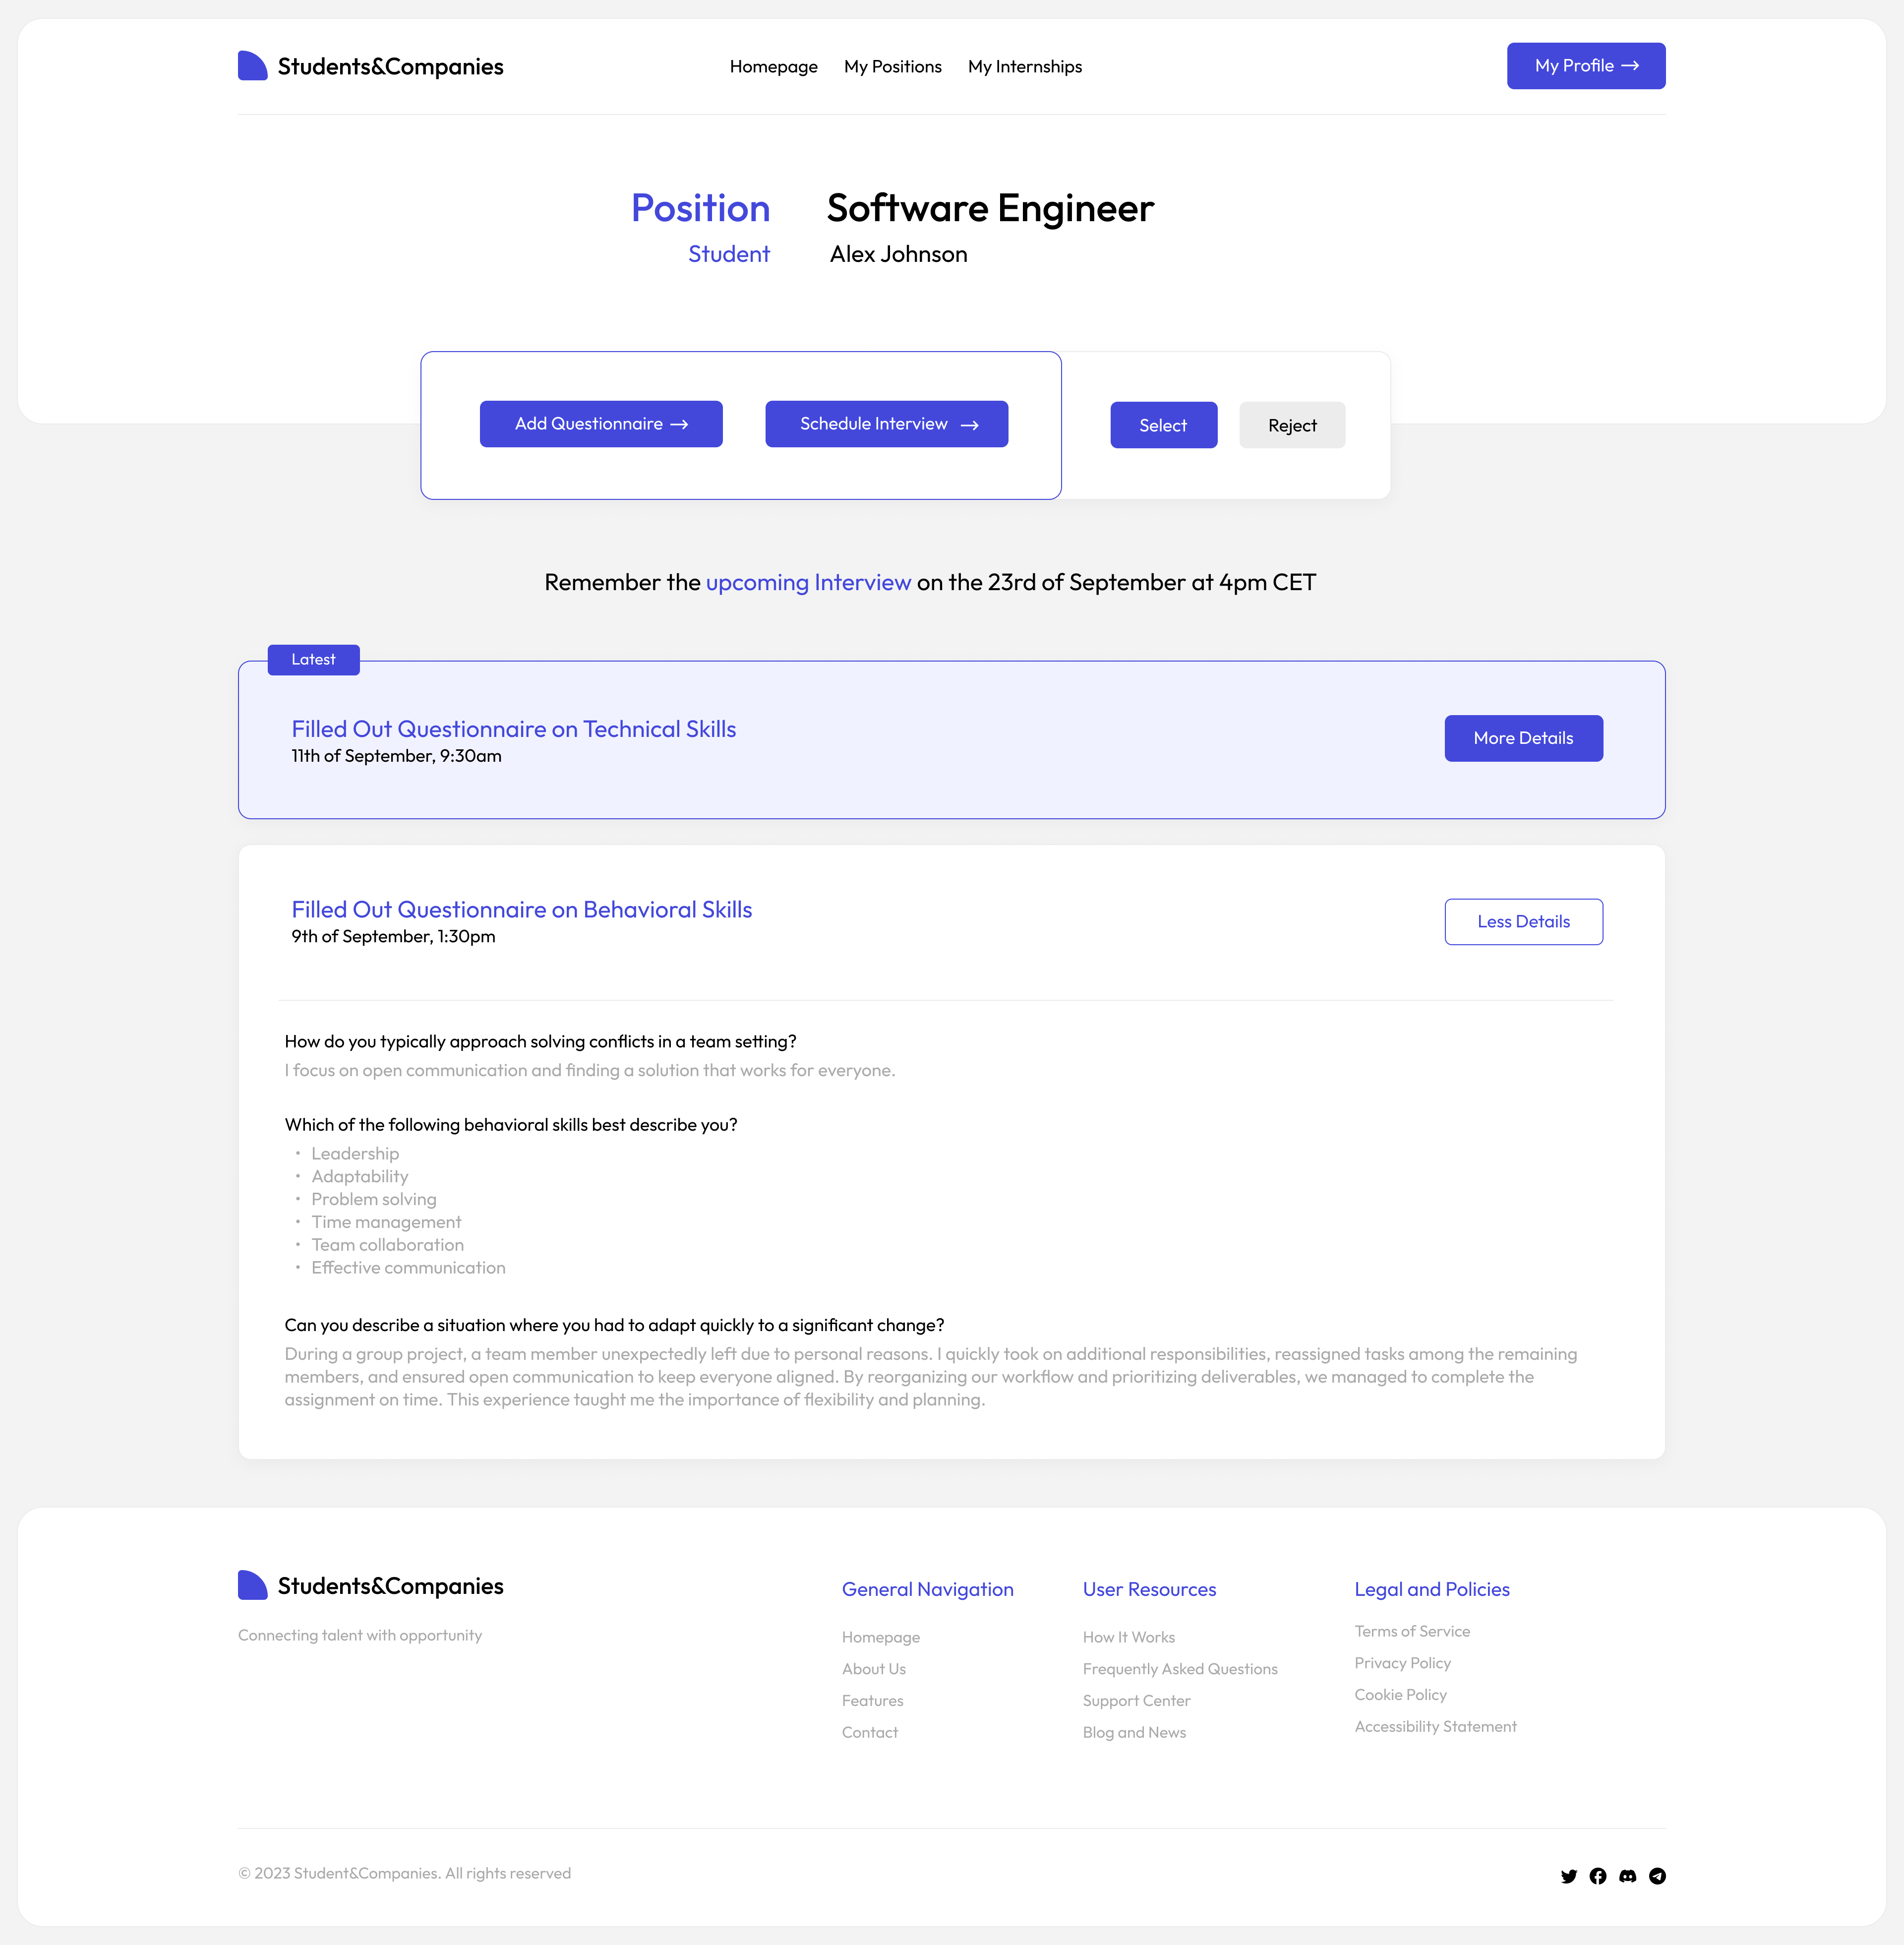
\includegraphics[width=16cm]{images/selected-pages/company-position-page.png}
    \caption{Company position page}
\end{figure}

\subsection{University Internship Page}
The university internship page ensures consistency with the platform through a standardized header and footer design.
The body allows universities to view comments on the internship or write them to report progress or address concerns.
These are displayed in an organized list, where each entry can be expanded to review the full content.
This interface facilitates communication between students, companies and universities, ensuring internships remain productive and beneficial for all parties involved.

\begin{figure}[h]
    \centering
    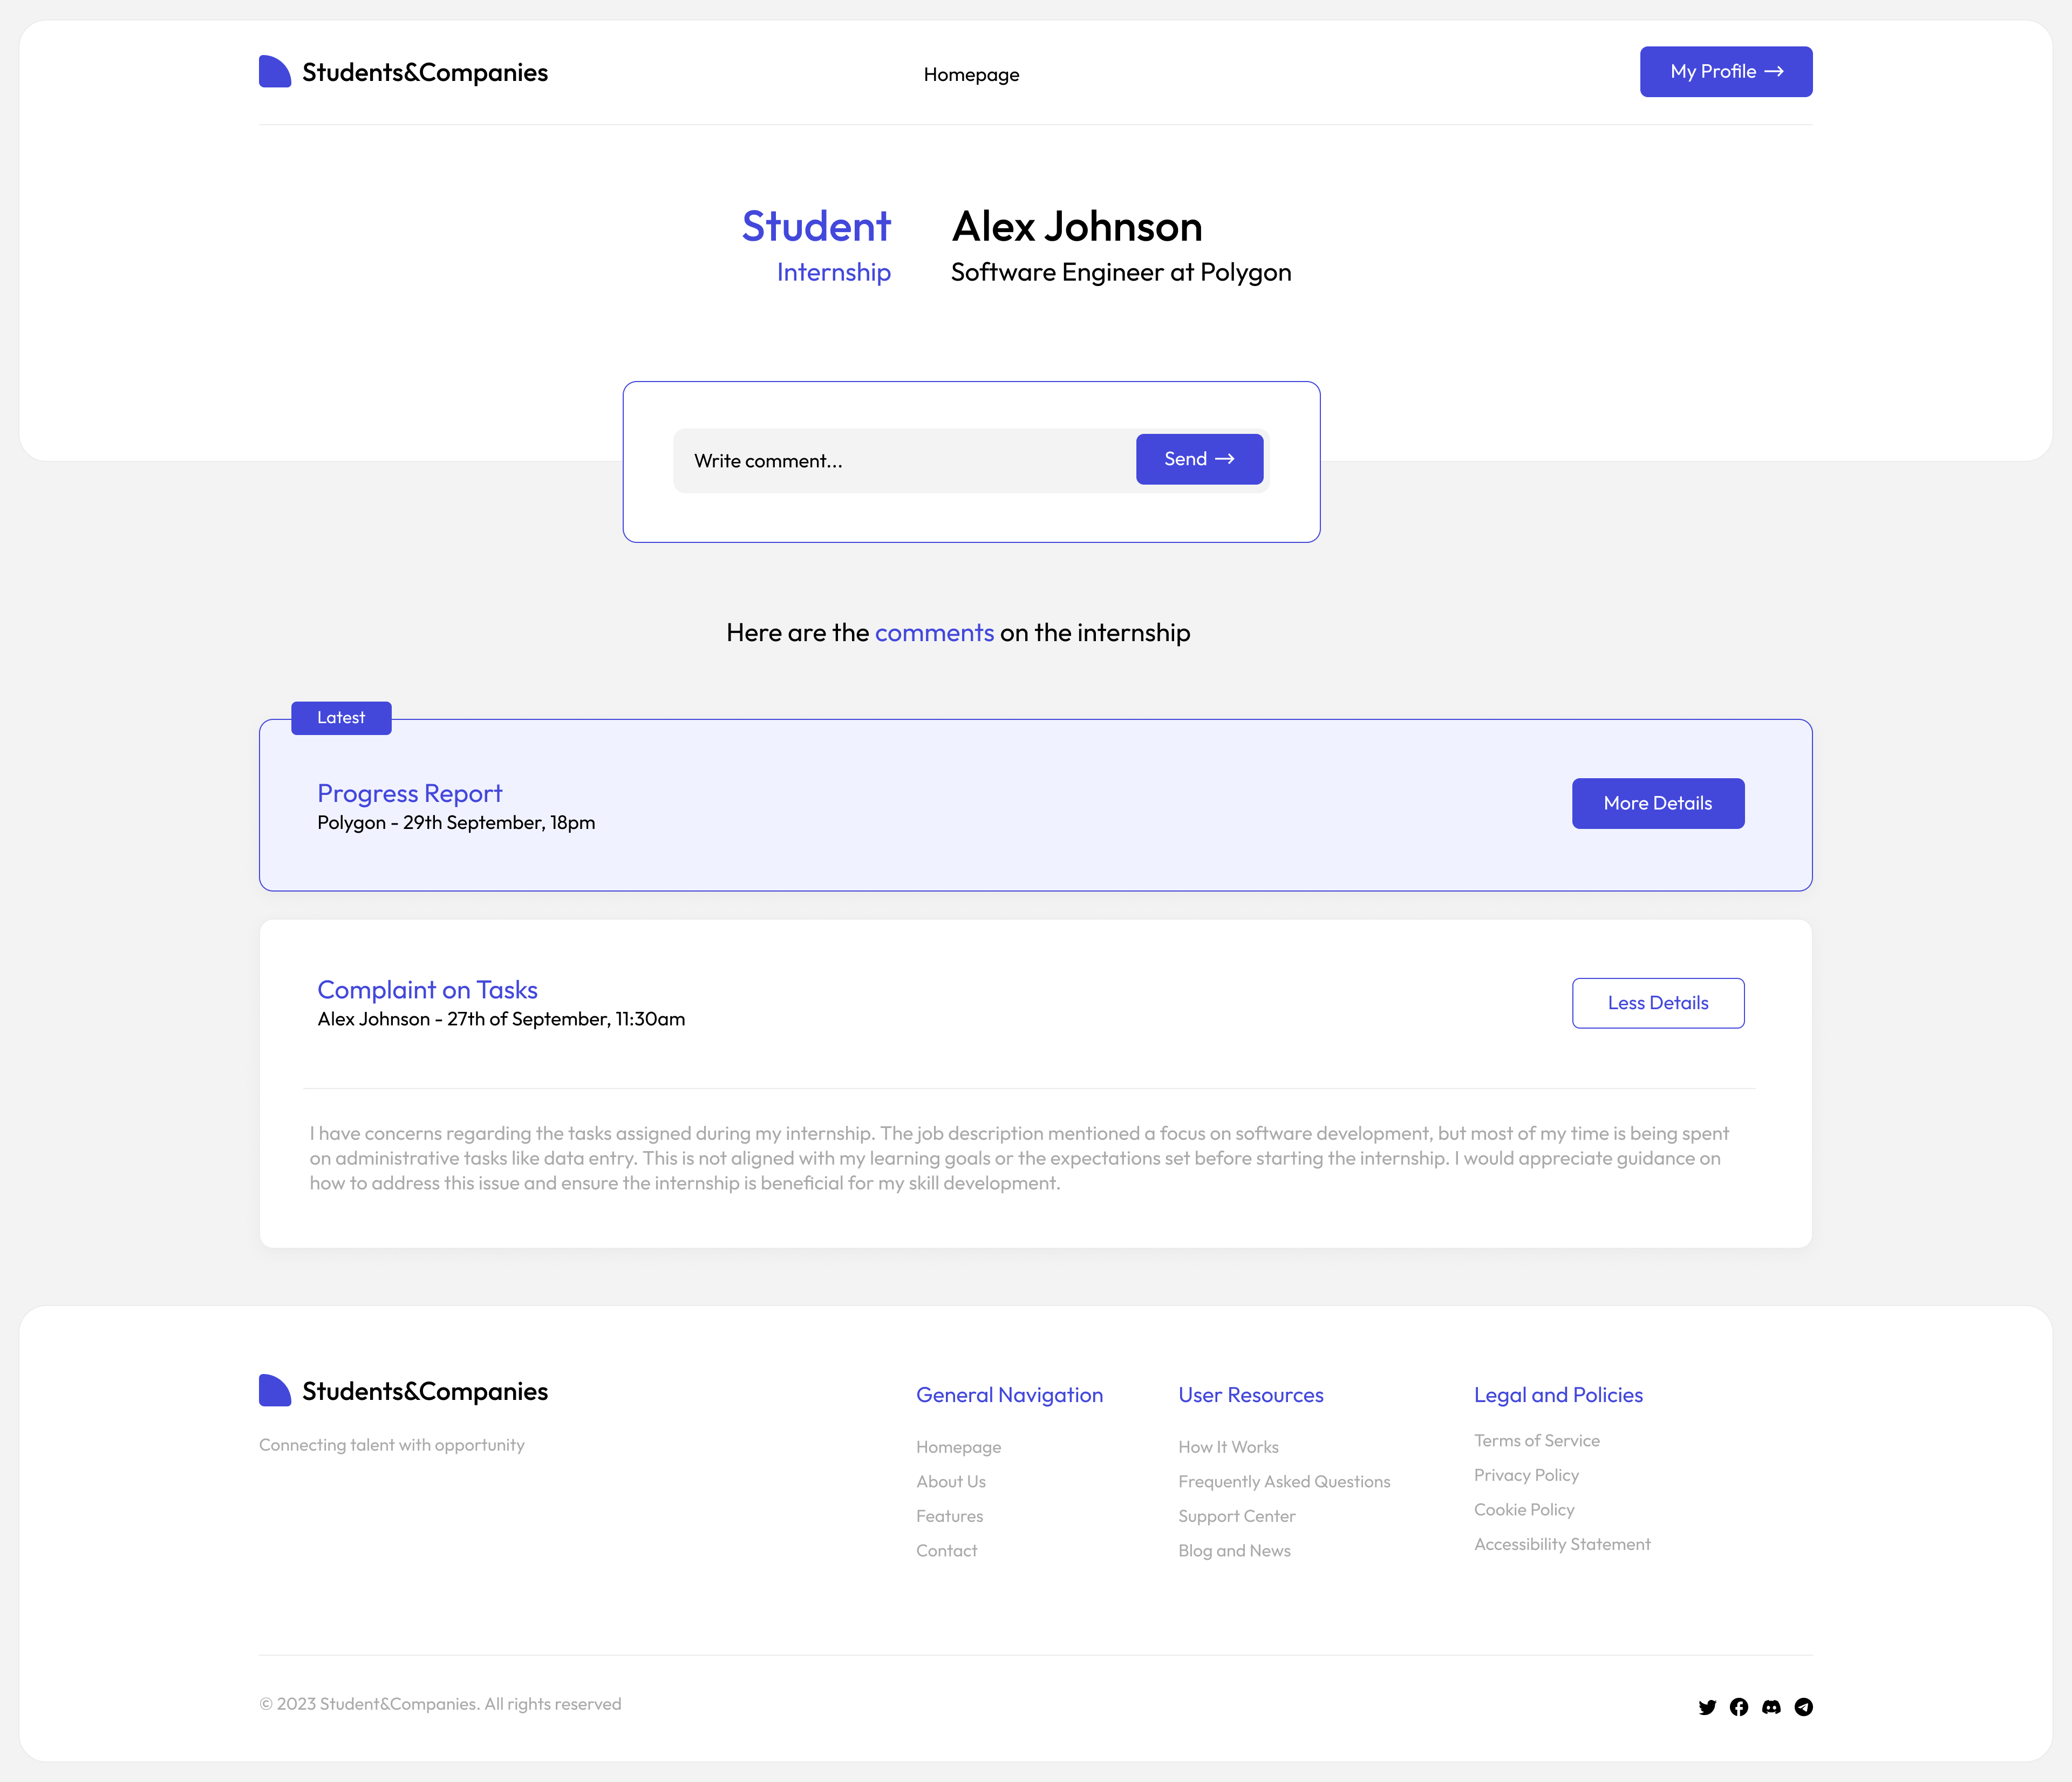
\includegraphics[width=16cm]{images/selected-pages/university-internship-page.png}
    \caption{University internship page}
\end{figure}


\chapter{Requirements Traceability}
This chapter illustrates how the requirements specified in the requirements analysis and specification document \cite{carraracurrodossi2024} are assigned to the submanagers.
The mapping employs three-letter acronyms for clarity and consistency; for example, User Signup Submanager is abbreviated as USS.
The table below presents the correspondence between the requirements and their respective submanagers.

\newcounter{r}
\setcounter{r}{1}
\newcommand{\rc}{\ther\stepcounter{r}}
\renewcommand{\arraystretch}{1.5}
\begin{longtable}{|c|p{10.5cm}|}
    \hline \rowcolor{polimiblue!40}
    \textbf{ID} & \textbf{Submanager} \\ \hline
    R\rc & USS, NFS, NDS \\ \hline
    R\rc & UMS, NFS, NDS \\ \hline
    R\rc & ULS \\ \hline
    R\rc & ULS \\ \hline
    R\rc & UMS \\ \hline
    R\rc & UMS \\ \hline
    R\rc & UMS \\ \hline
    R\rc & UMS \\ \hline
    R\rc & PSS \\ \hline
    R\rc & PSS \\ \hline
    R\rc & PSS \\ \hline
    R\rc & SAS, NFS, NDS \\ \hline
    R\rc & SAS \\ \hline
    R\rc & RMS \\ \hline
    R\rc & RMS \\ \hline
    R\rc & RFS \\ \hline
    R\rc & SAS \\ \hline
    R\rc & SAS \\ \hline
    R\rc & SQS \\ \hline
    R\rc & SIS \\ \hline
    R\rc & SIS \\ \hline
    R\rc & SAS \\ \hline
    R\rc & IPS \\ \hline
    R\rc & IPS \\ \hline
    R\rc & ICS \\ \hline
    R\rc & ICS \\ \hline
    R\rc & USS, NFS, NDS \\ \hline
    R\rc & UMS, NFS, NDS \\ \hline
    R\rc & ULS \\ \hline
    R\rc & ULS \\ \hline
    R\rc & UMS \\ \hline
    R\rc & PPS \\ \hline
    R\rc & PMS \\ \hline
    R\rc & PMS \\ \hline
    R\rc & PMS \\ \hline
    R\rc & PSS \\ \hline
    R\rc & RMS \\ \hline
    R\rc & RMS \\ \hline
    R\rc & RFS \\ \hline
    R\rc & SAS \\ \hline
    R\rc & SAS \\ \hline
    R\rc & SQS \\ \hline
    R\rc & SQS \\ \hline
    R\rc & SIS \\ \hline
    R\rc & SAS \\ \hline
    R\rc & IPS \\ \hline
    R\rc & IPS \\ \hline
    R\rc & ICS \\ \hline
    R\rc & ICS \\ \hline
    R\rc & USS, NFS, NDS \\ \hline
    R\rc & UMS, NFS, NDS \\ \hline
    R\rc & ULS \\ \hline
    R\rc & ULS \\ \hline
    R\rc & IPS \\ \hline
    R\rc & IPS \\ \hline
    R\rc & IPS \\ \hline
    R\rc & IPS \\ \hline
    R\rc & IPS \\ \hline
    R\rc & ICS \\ \hline
    R\rc & ICS \\ \hline
    R\rc & RMS, NFS, NDS \\ \hline
    R\rc & RMS, NFS, NDS \\ \hline
    R\rc & RMS, NFS, NDS \\ \hline
    R\rc & RMS, NFS, NDS \\ \hline
    R\rc & SAS, NFS, NDS \\ \hline
    R\rc & SAS, NFS, NDS \\ \hline
    R\rc & SQS, NFS, NDS \\ \hline
    R\rc & SQS, NFS, NDS \\ \hline
    R\rc & SIS, NFS, NDS \\ \hline
    R\rc & SIS, NFS, NDS \\ \hline
    R\rc & SIS, NFS, NDS \\ \hline
    R\rc & SAS, NFS, NDS \\ \hline
    R\rc & IPS, NFS, NDS \\ \hline
    R\rc & IPS, NFS, NDS \\ \hline
    R\rc & IPS, NFS, NDS \\ \hline
    R\rc & ICS, NFS, NDS \\ \hline
    R\rc & ICS, NFS, NDS \\ \hline
    R\rc & ICS, NFS, NDS \\ \hline
\caption{Requirements traceability}
\end{longtable}


\chapter{Implementation, Integration and Test Plan}
This chapter dives deep into how Students\&Companies is implemented, integrated and tested.
The chosen approach follows a bottom-up strategy.
It begins with developing and testing foundational elements before integrating the rest of the system.
This gradual process focuses on the independent development of basic modules, which are tested in isolation before being integrated into the larger system.
This independence eliminates the need to consider the entire system upfront, making it easier and faster to address issues and apply changes.
A key factor of this method is the usage of drivers, short tests that simulate the inputs and interactions essential for checking individual modules.

The plan begins with the development and testing of base components, specifically the foundational submanagers within each manager.
Once these base submanagers are implemented and tested, the remaining ones for the same manager are integrated. 
To ensure clarity, when all submanagers of a manager are integrated, they are represented in the diagrams through their respective manager component.

The first step is to implement and test the model.

\begin{figure}[h]
    \centering
    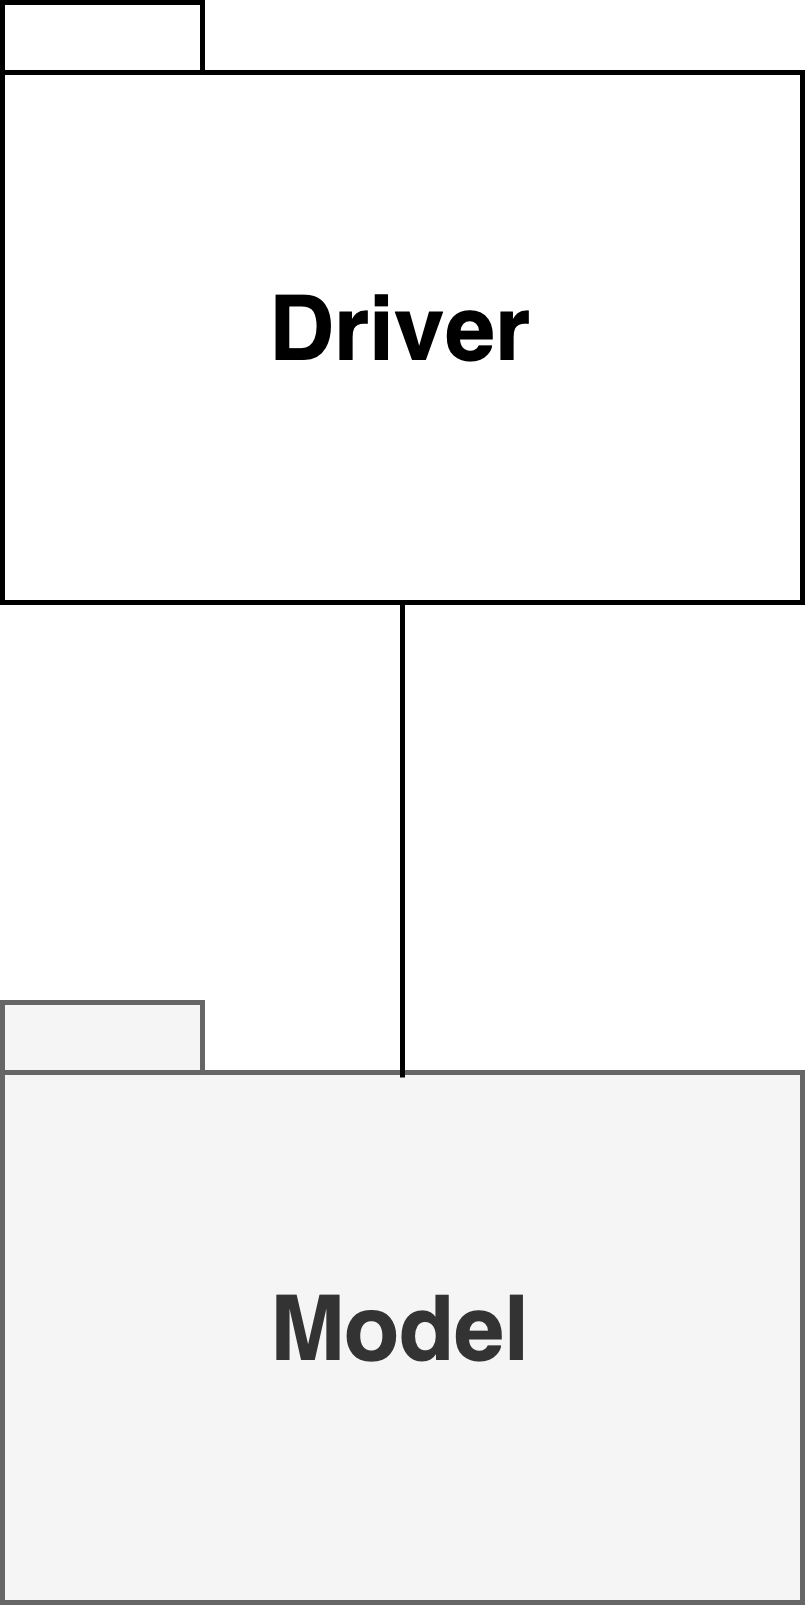
\includegraphics[width=2.5cm]{images/implementation-diagrams/step-1.png}
    \caption{Implementation step 1}
\end{figure}

\newpage
The development proceeds to step two with the user signup and login submanagers.

\begin{figure}[h]
    \centering
    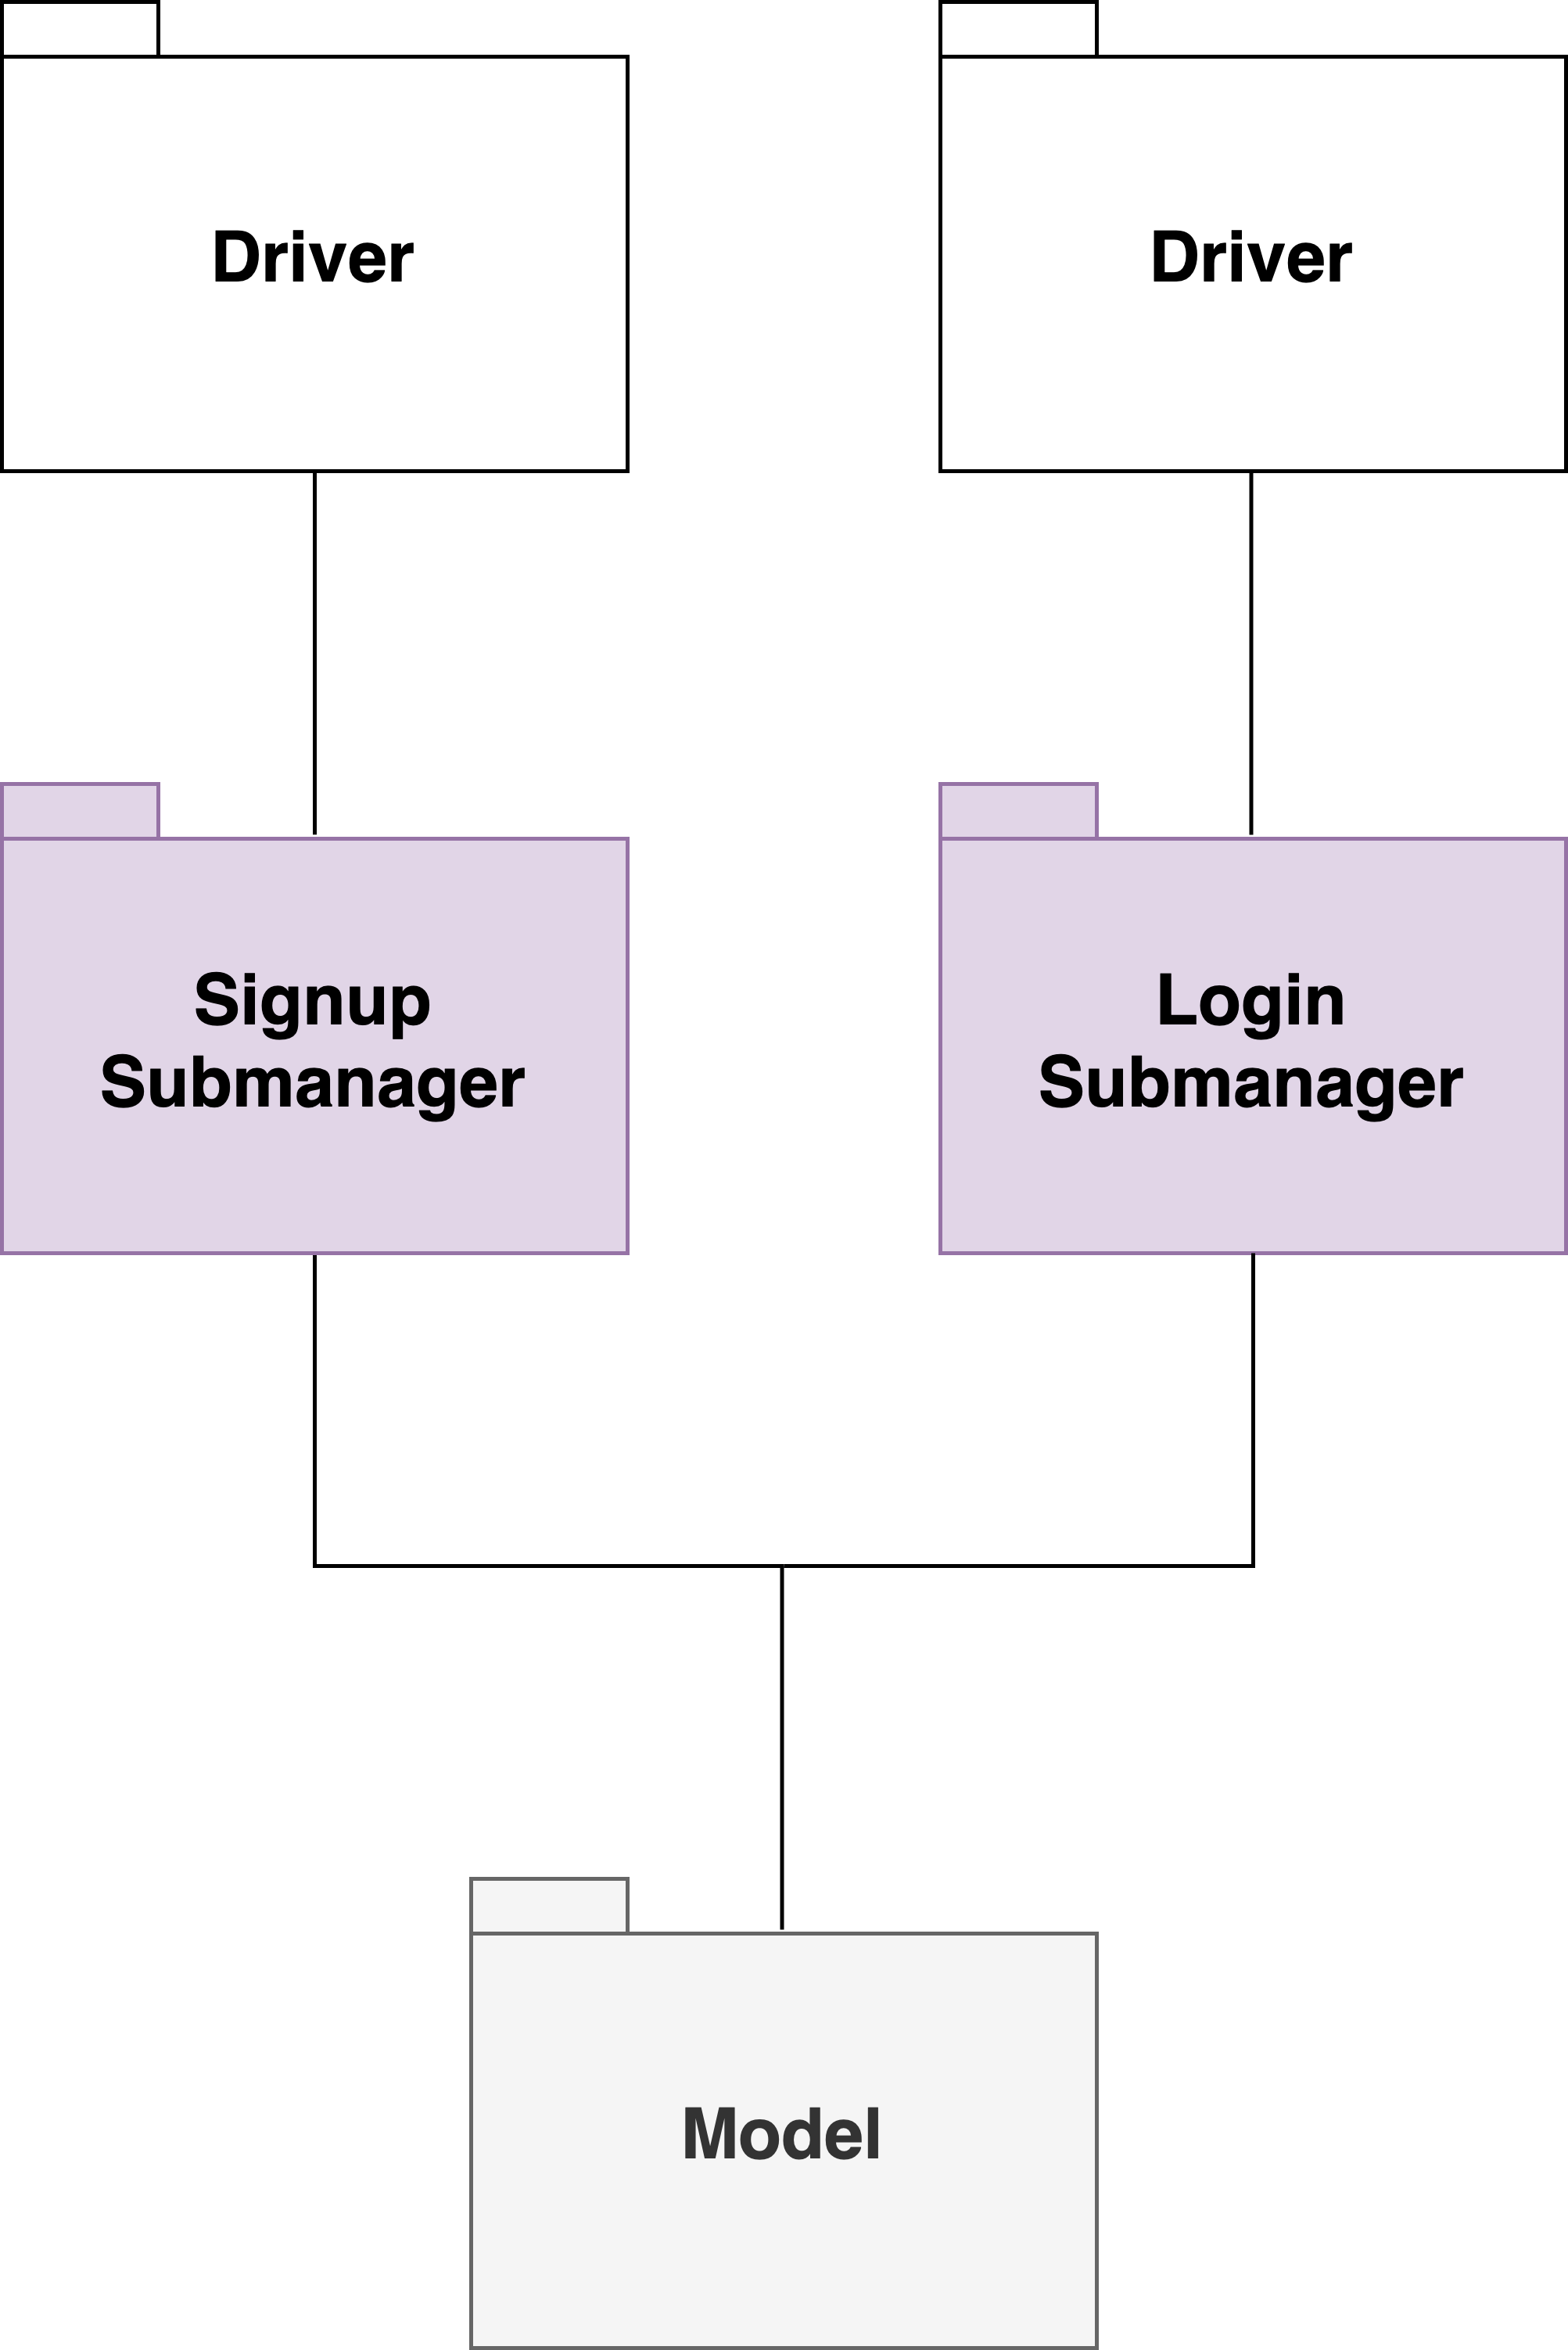
\includegraphics[width=6.5cm]{images/implementation-diagrams/step-2.png}
    \caption{Implementation step 2}
\end{figure}

\newpage
The user management submanager is integrated in the third step.

\begin{figure}[h]
    \centering
    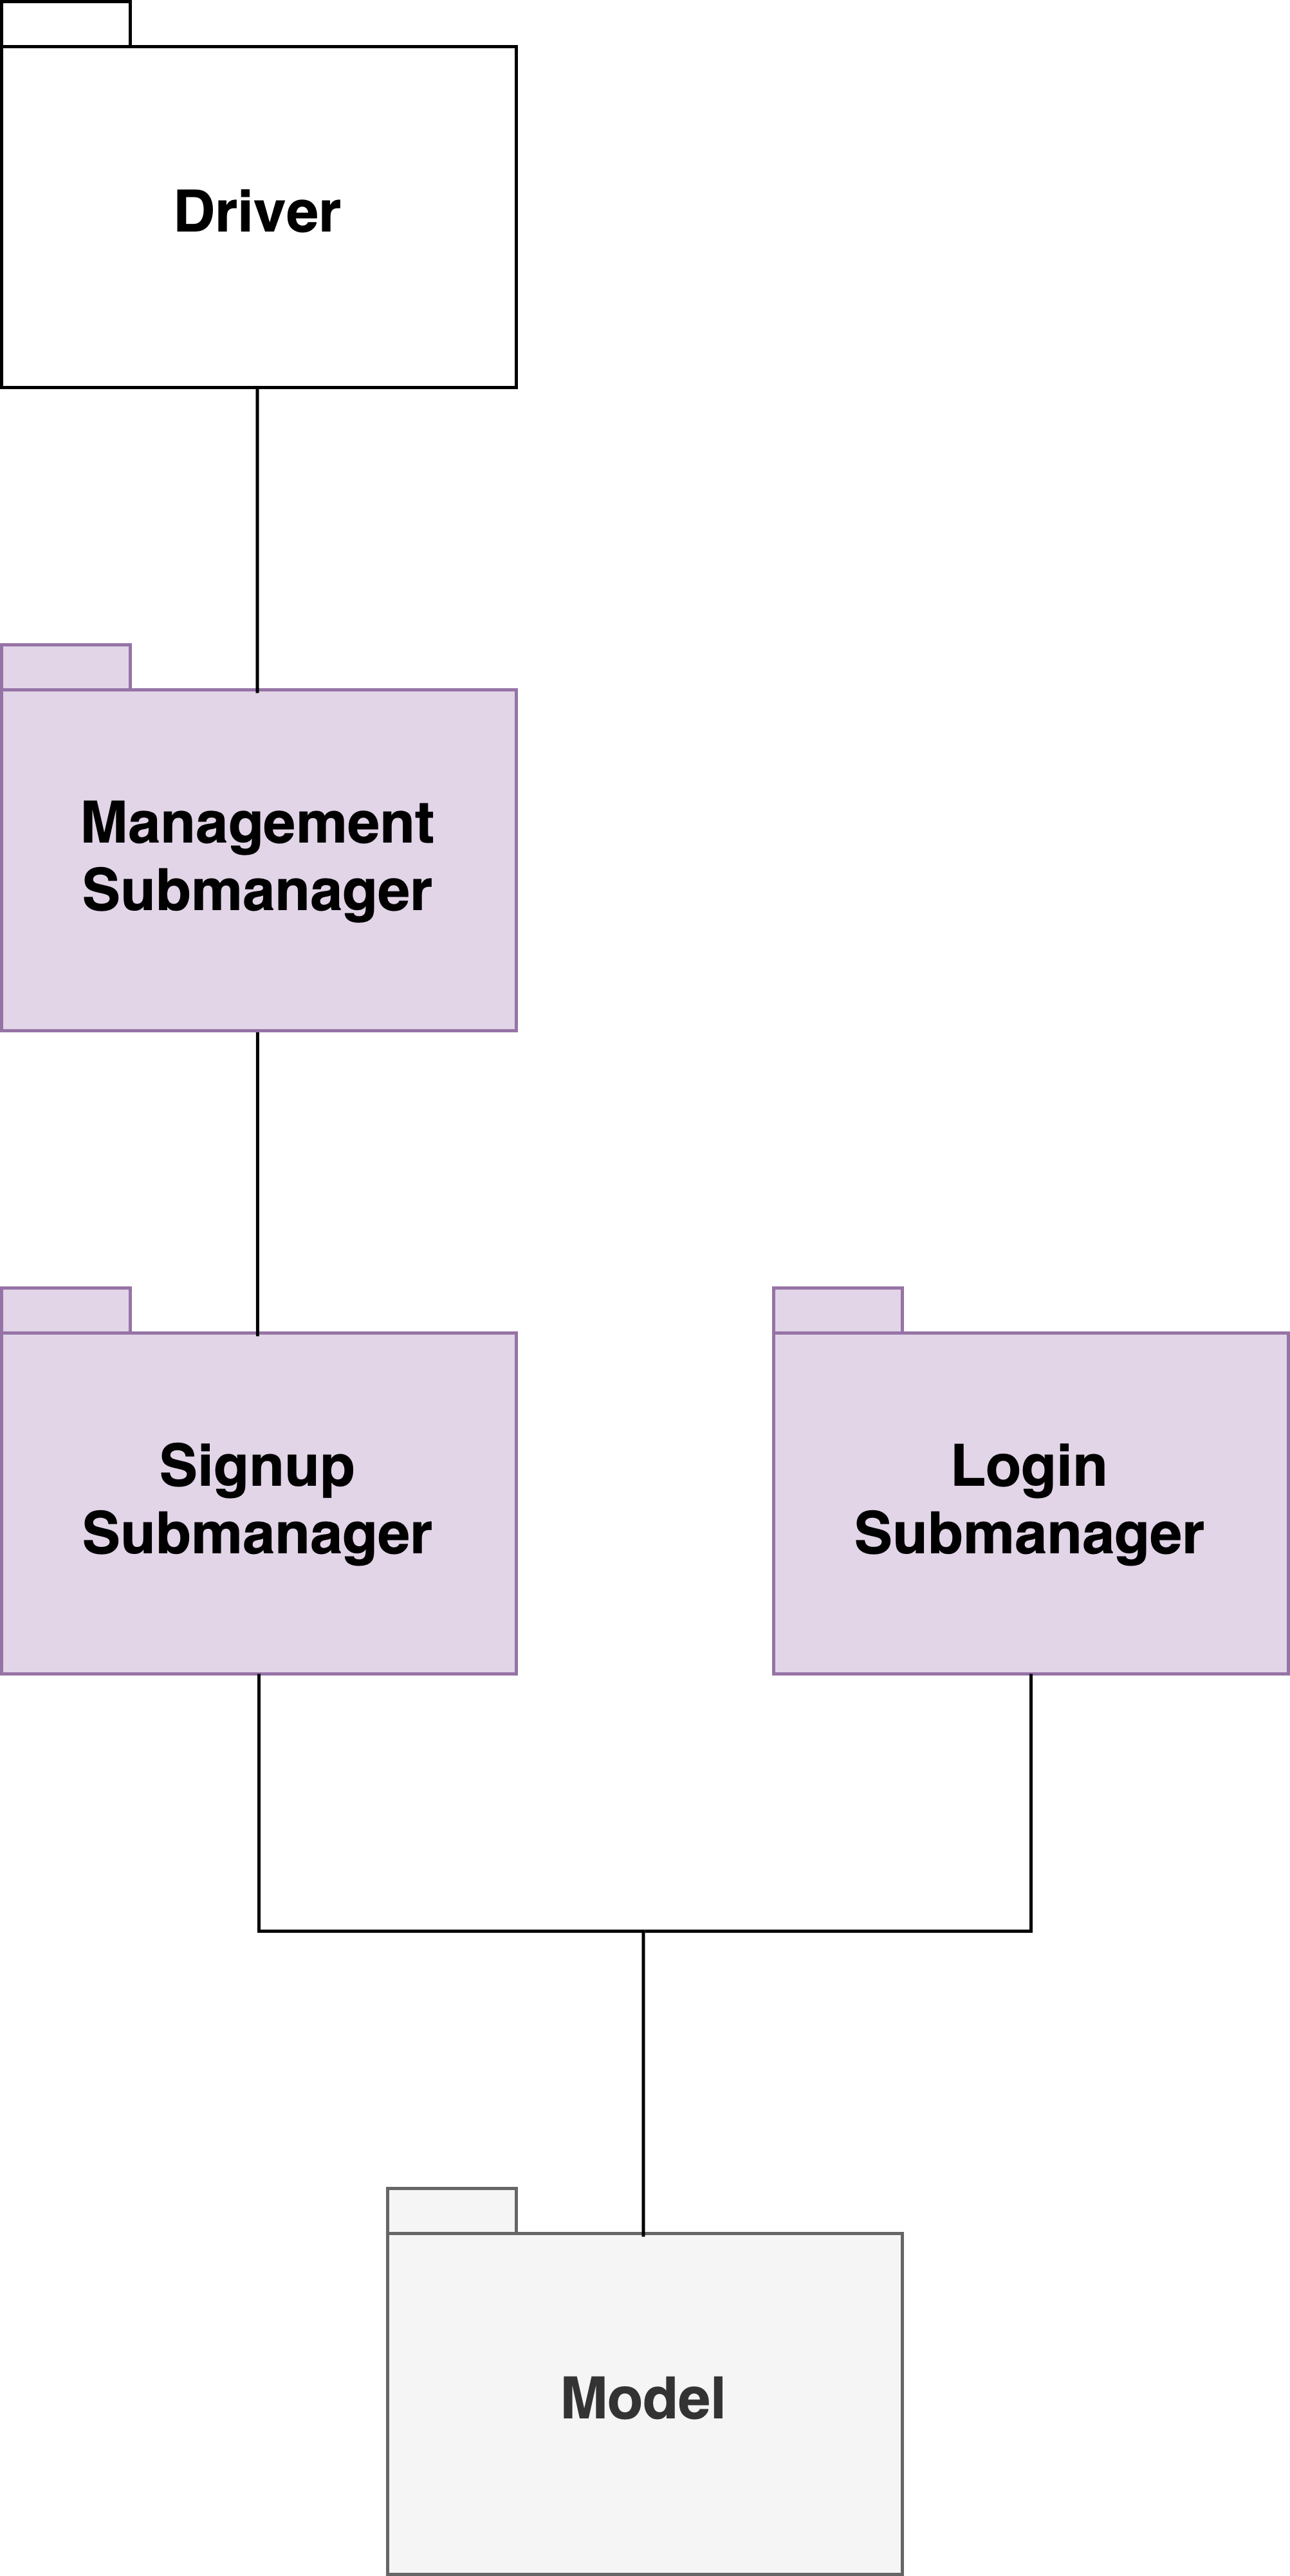
\includegraphics[width=6.5cm]{images/implementation-diagrams/step-3.png}
    \caption{Implementation step 3}
\end{figure}

\newpage
Step four applies the same pattern to the position posting and search submanagers.

\begin{figure}[h]
    \centering
    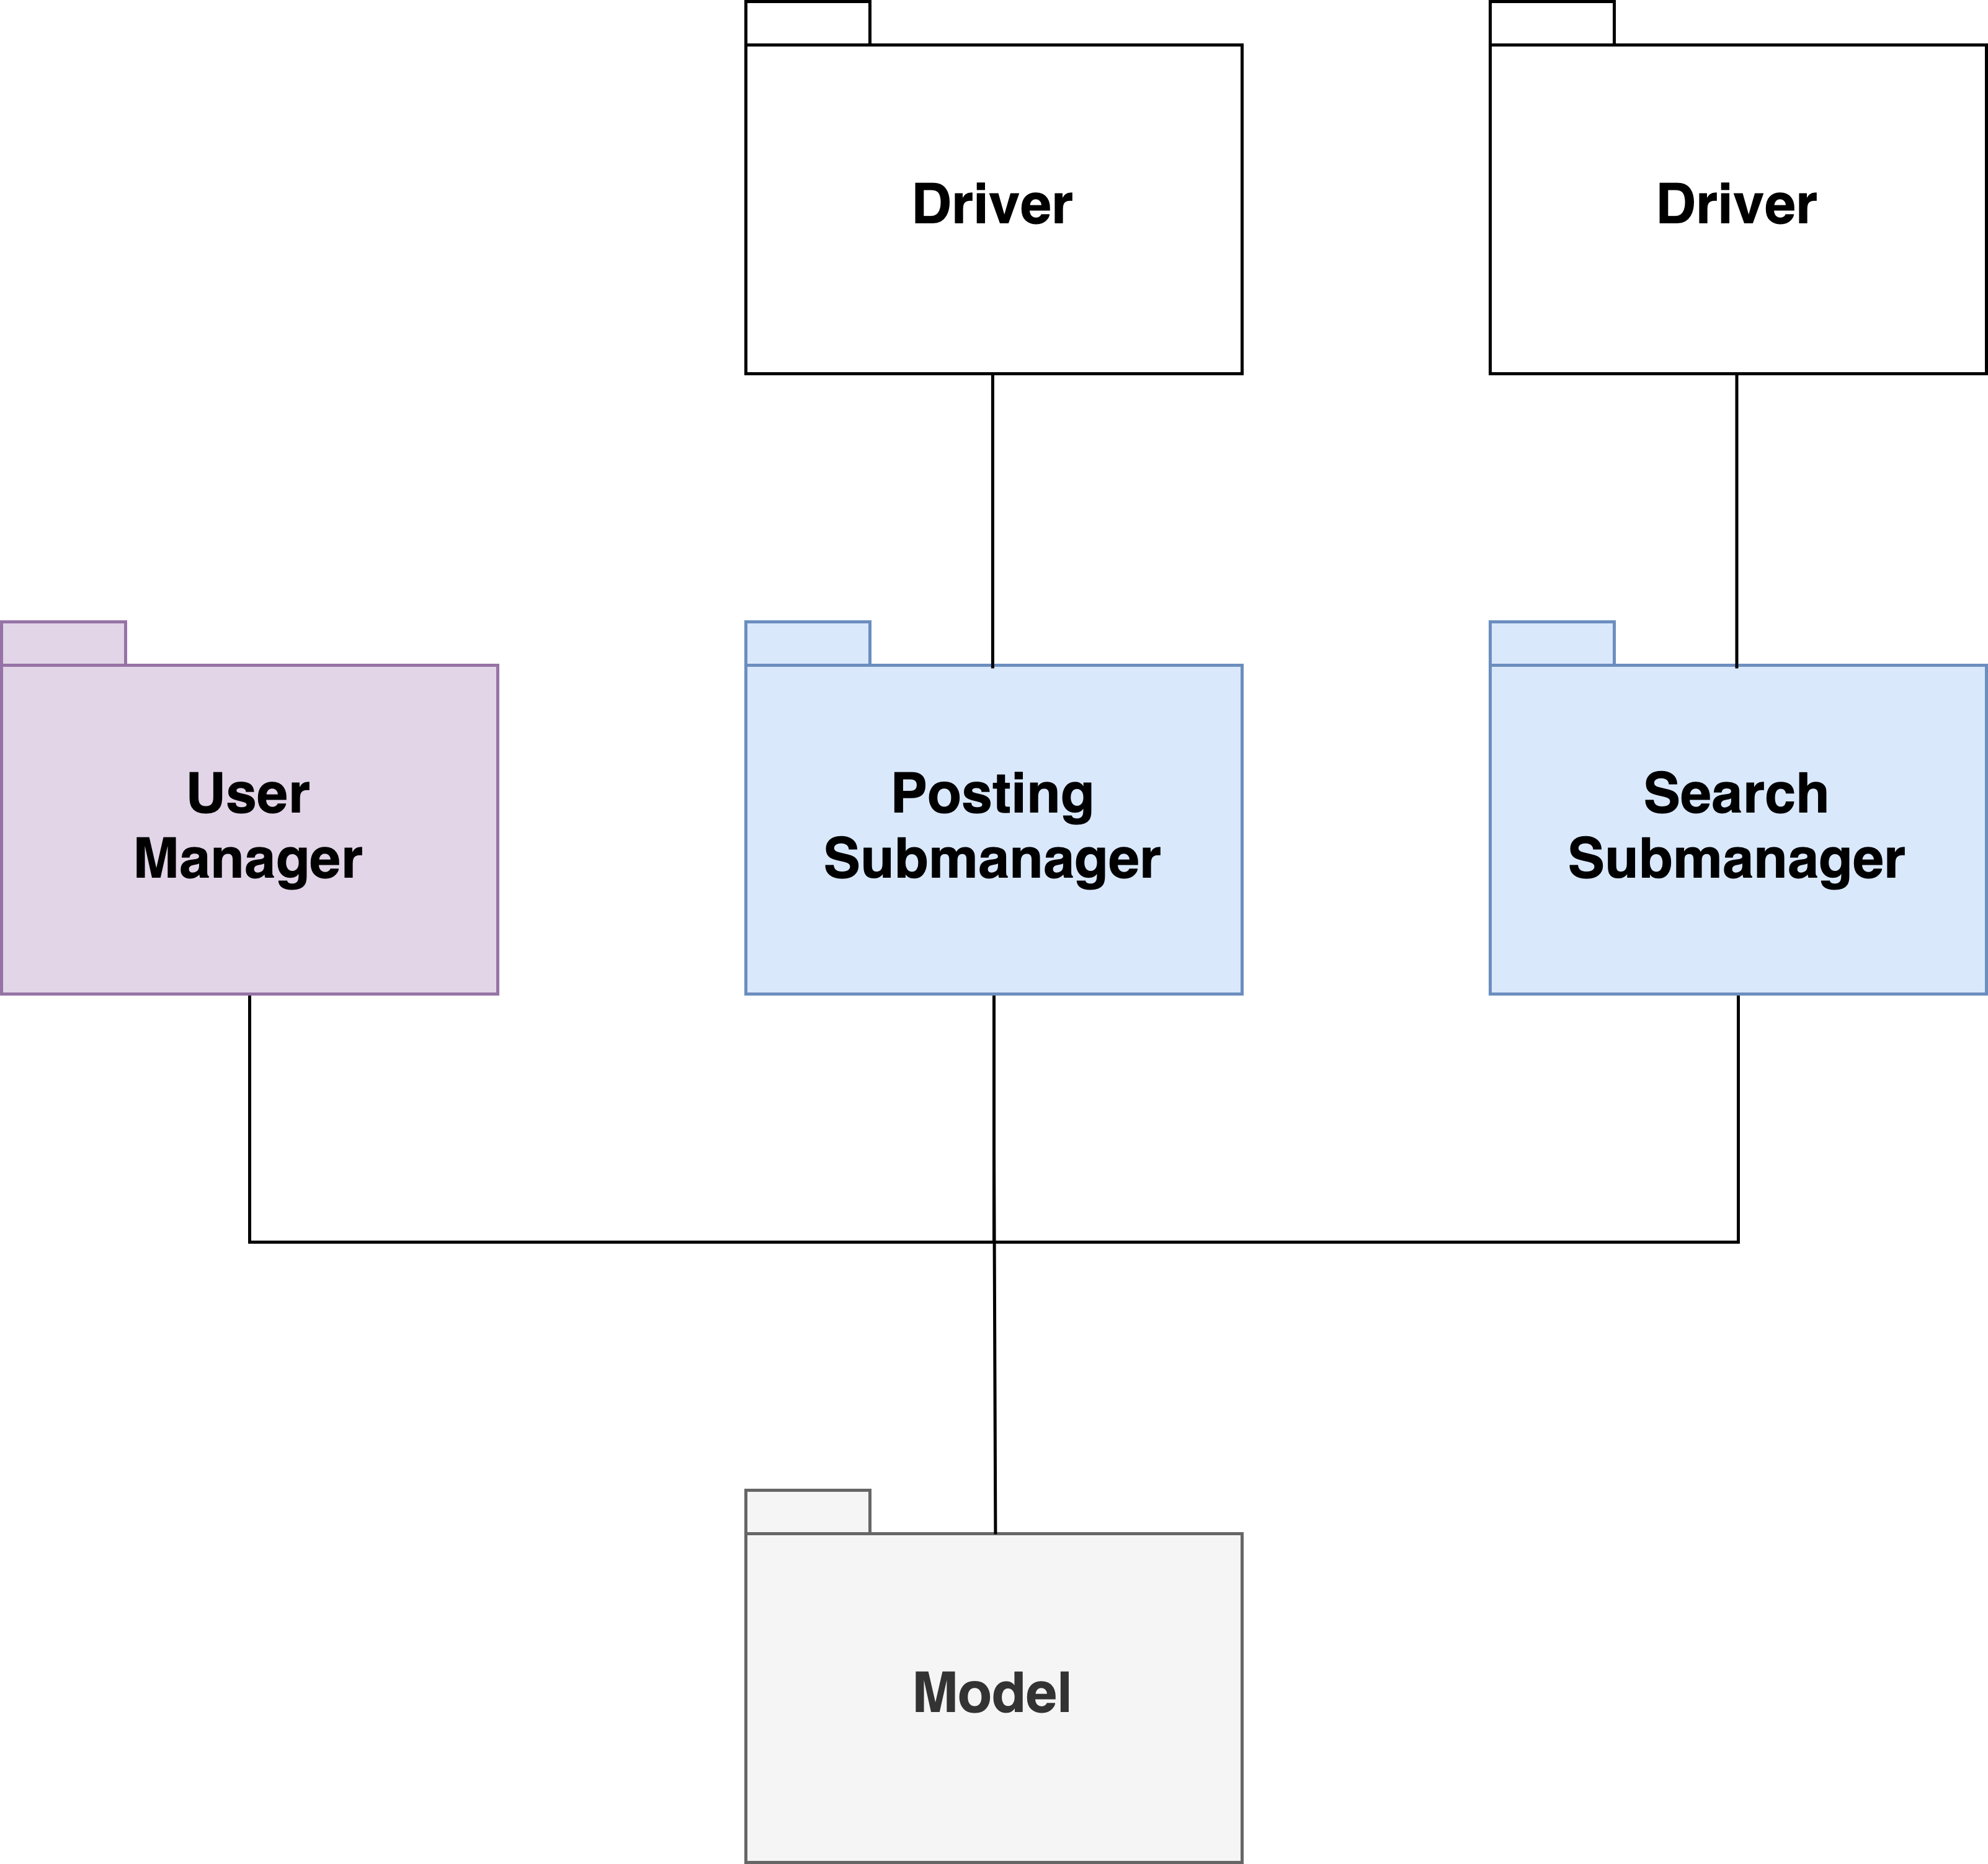
\includegraphics[width=10cm]{images/implementation-diagrams/step-4.png}
    \caption{Implementation step 4}
\end{figure}

\newpage
The position management submanager is integrated in the fifth step.

\begin{figure}[h]
    \centering
    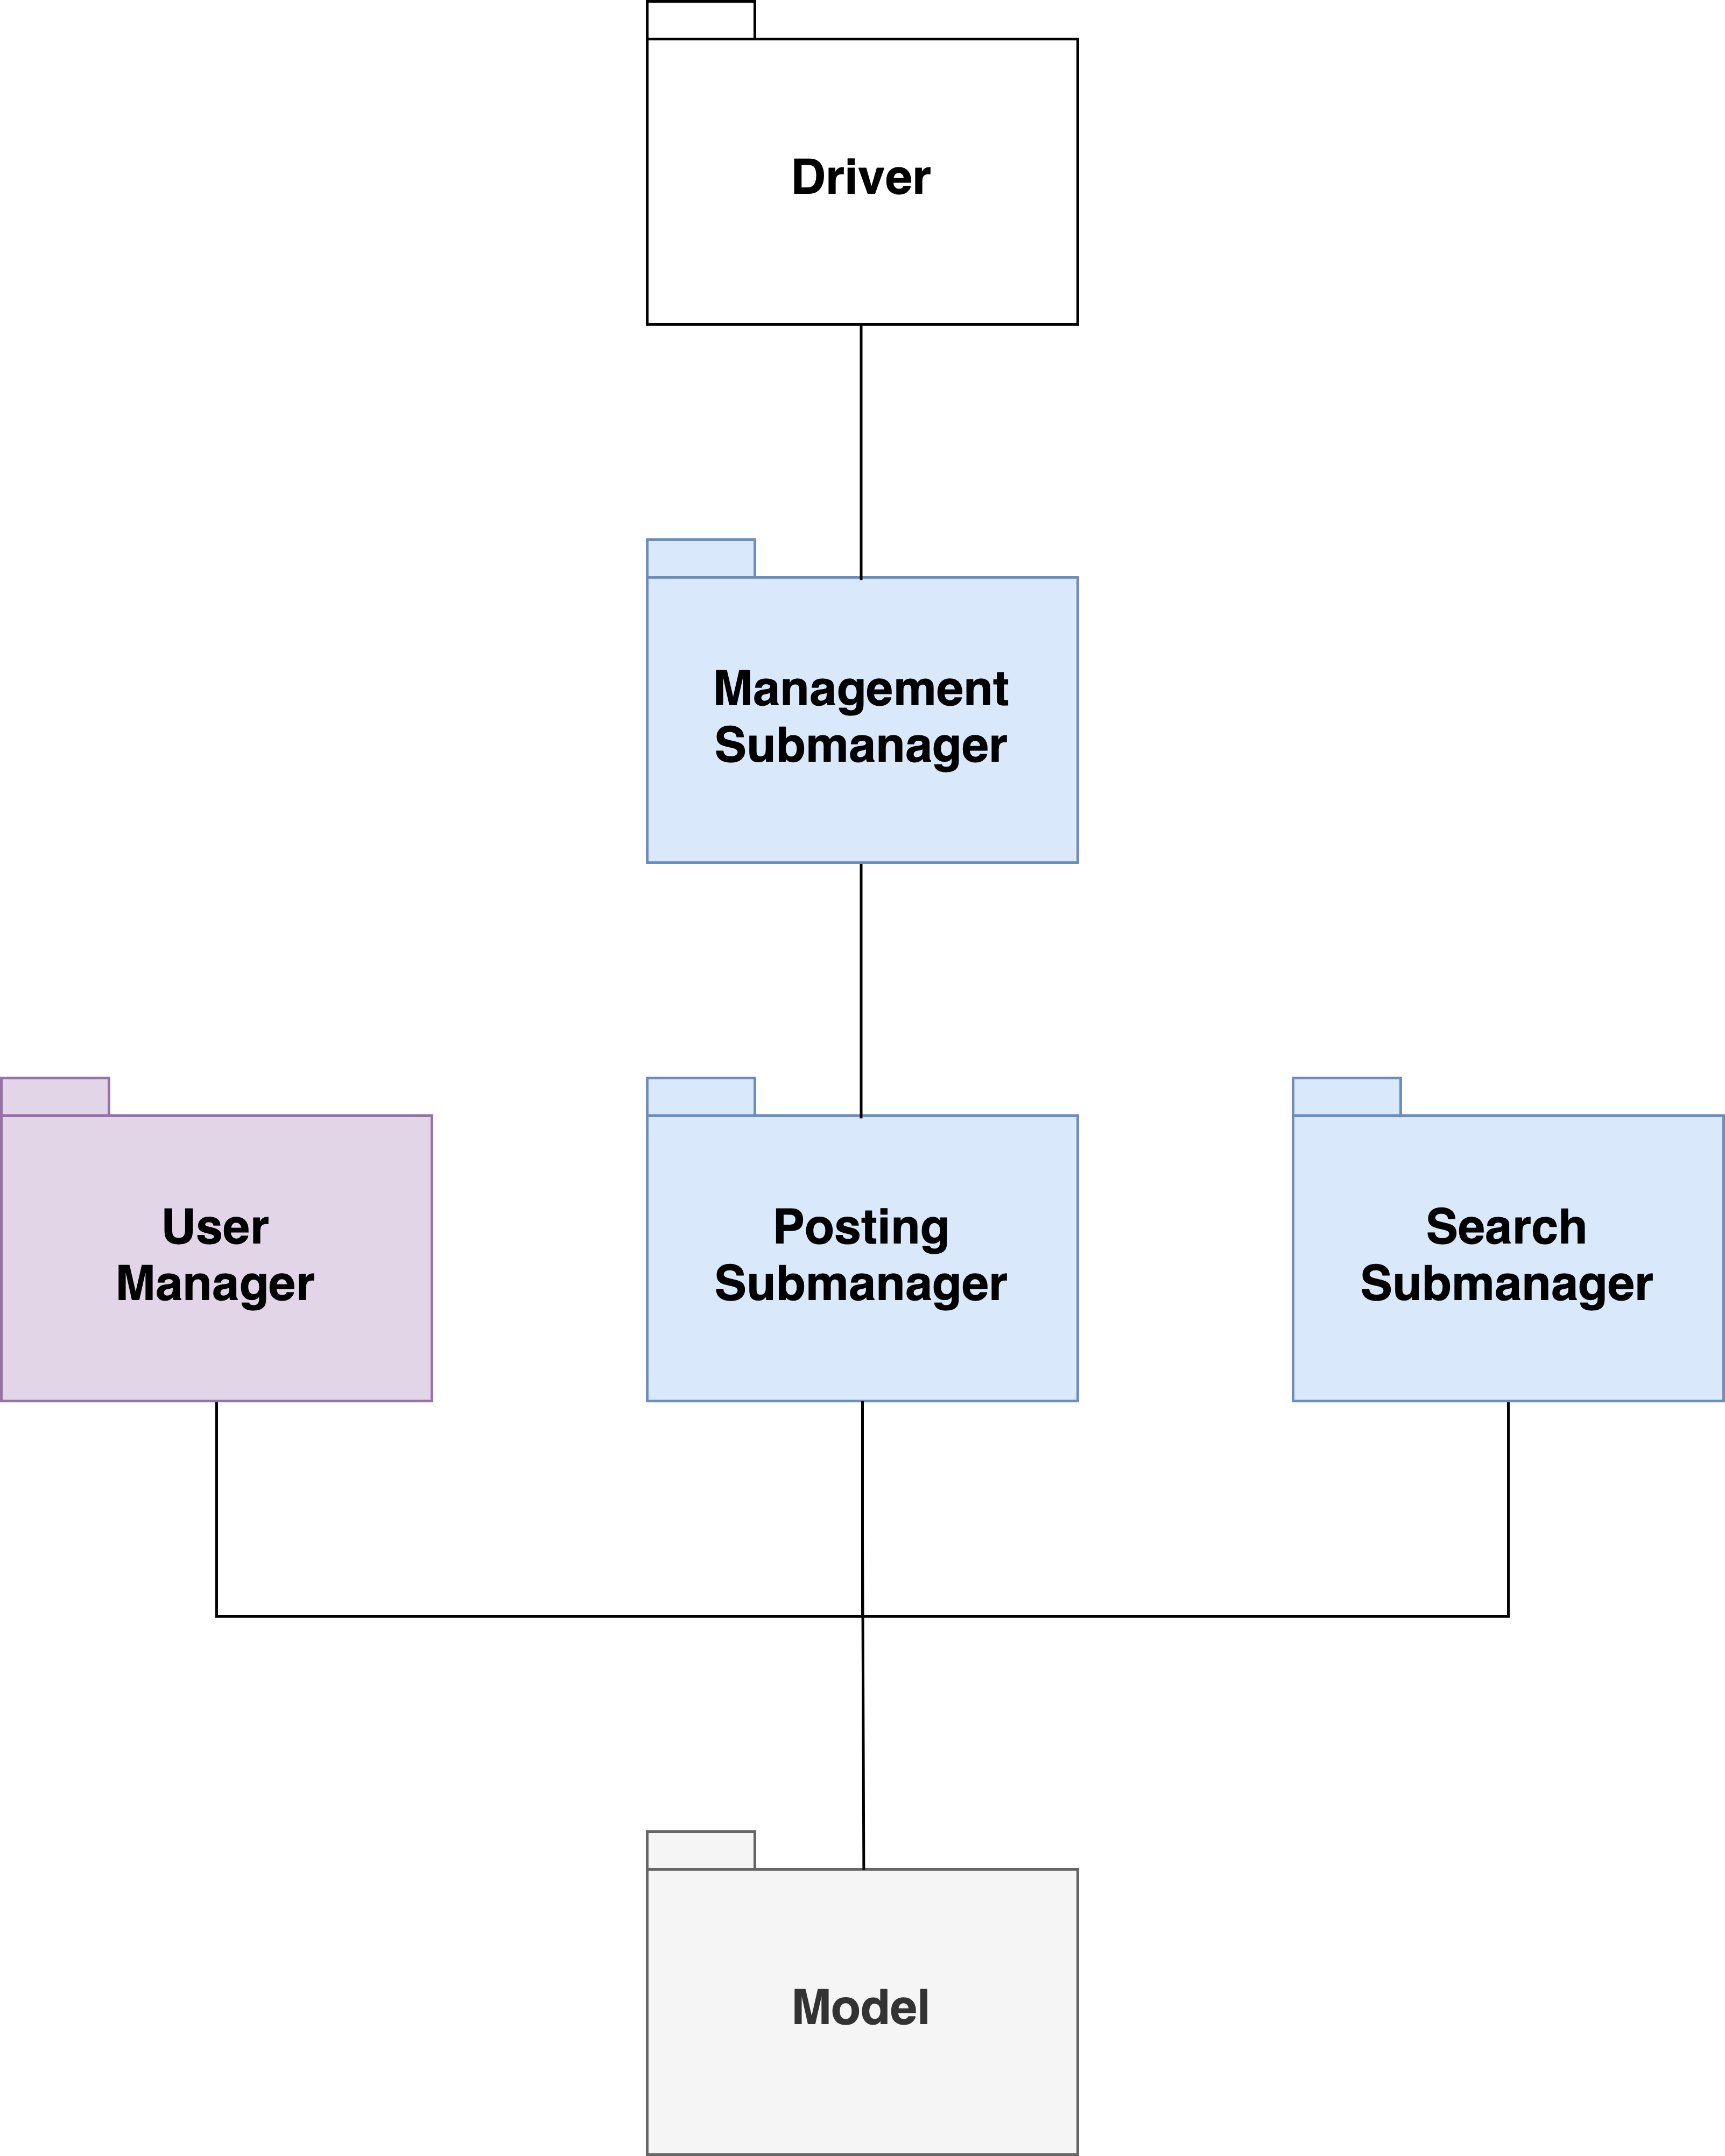
\includegraphics[width=10cm]{images/implementation-diagrams/step-5.png}
    \caption{Implementation step 5}
\end{figure}

\newpage
The development proceeds to step six with the recommendation submanagers.

\begin{figure}[h]
    \centering
    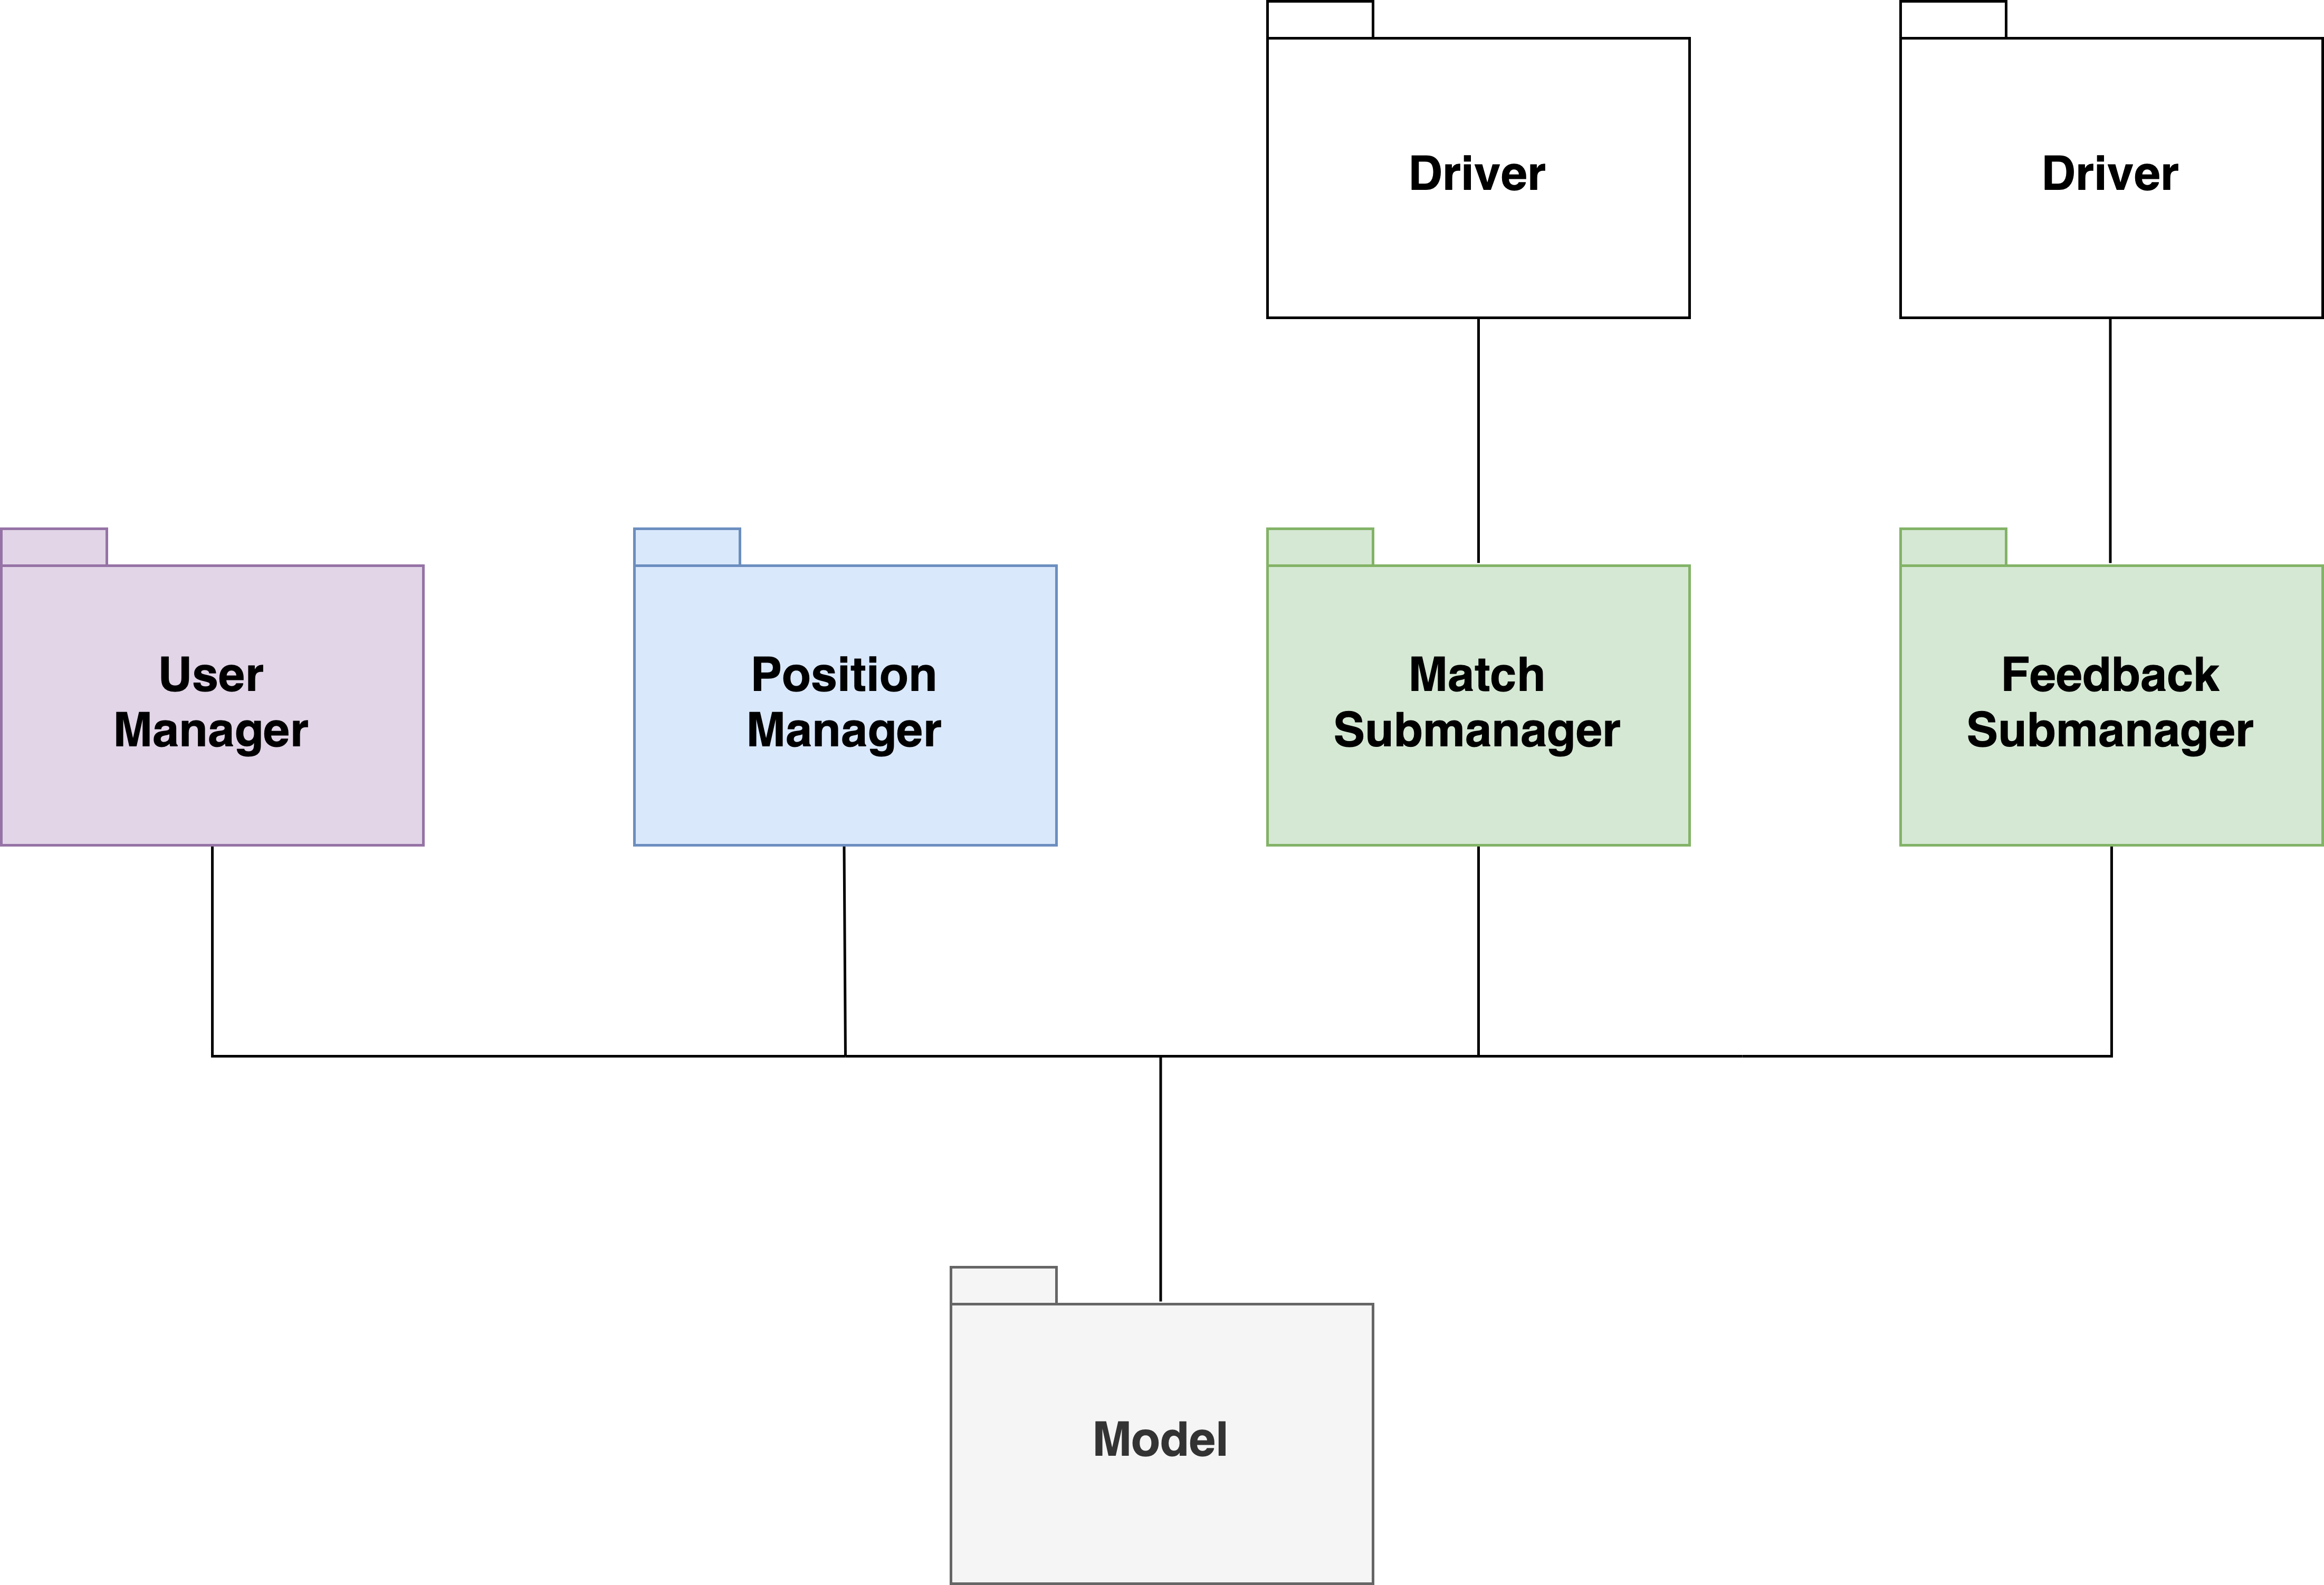
\includegraphics[width=13cm]{images/implementation-diagrams/step-6.png}
    \caption{Implementation step 6}
\end{figure}

\newpage
Step seven applies the same pattern to the selection application submanager.

\begin{figure}[h]
    \centering
    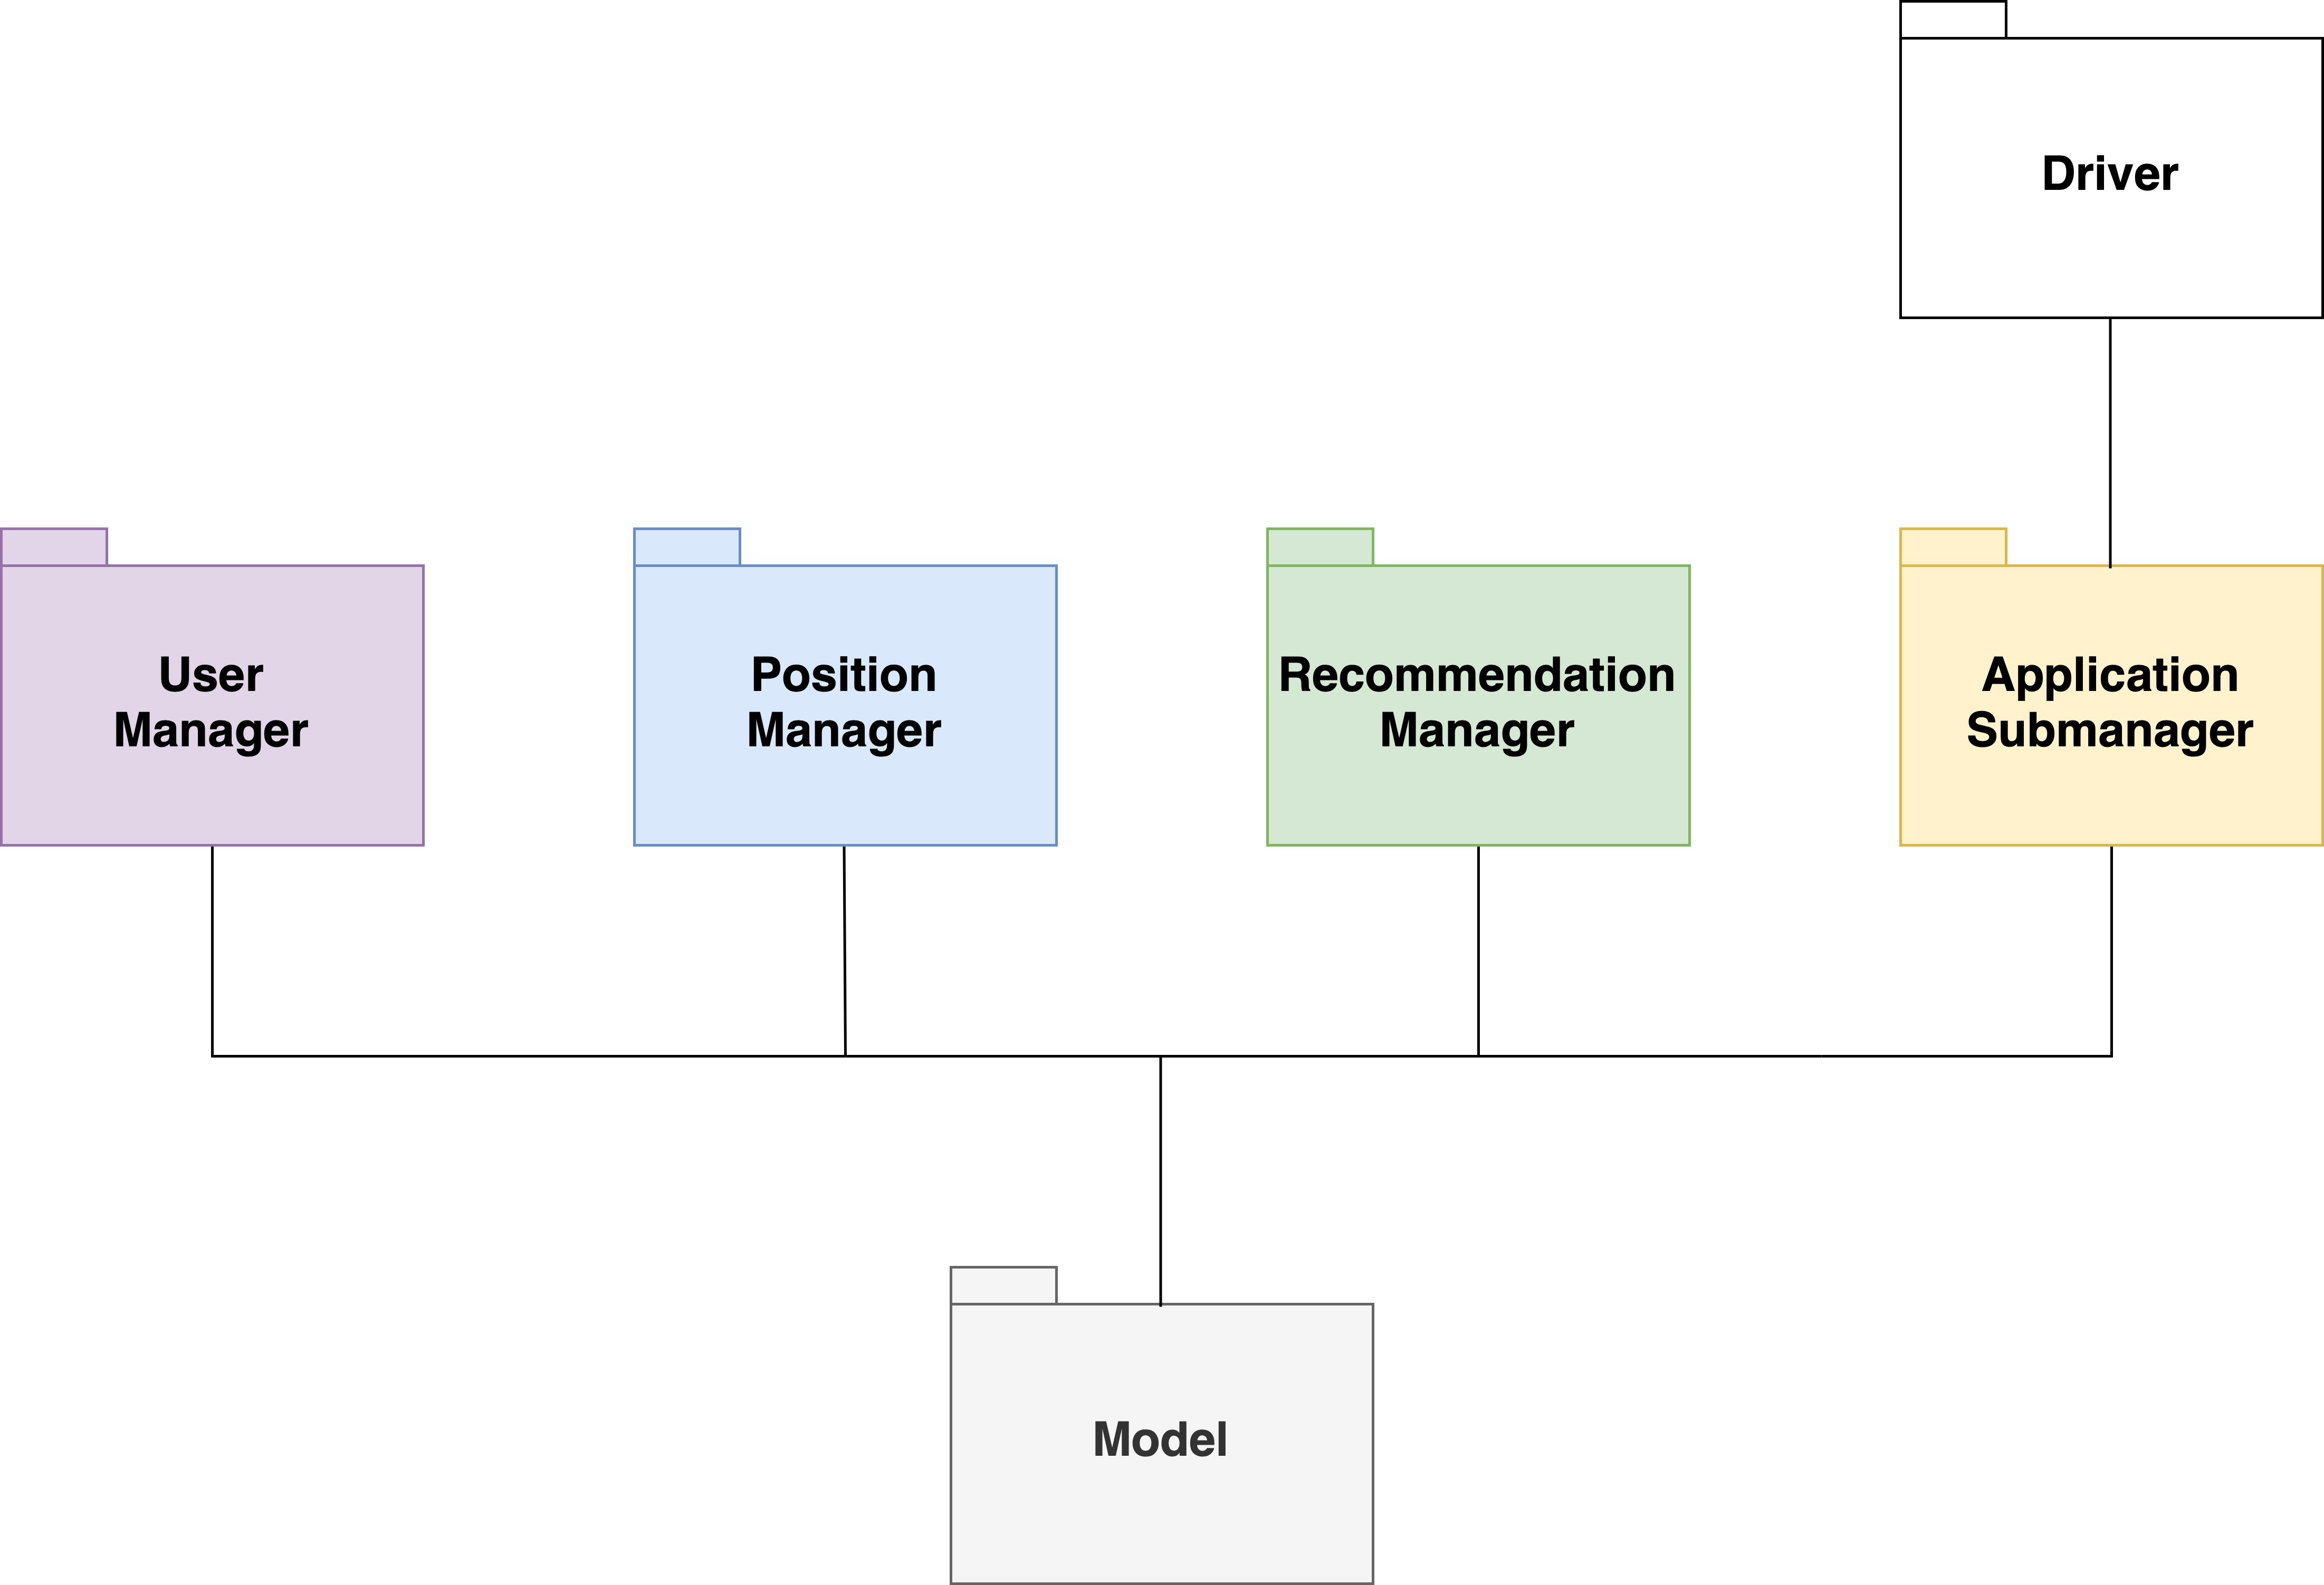
\includegraphics[width=13cm]{images/implementation-diagrams/step-7.png}
    \caption{Implementation step 7}
\end{figure}

\newpage
The selection interview and questionnaire submanagers are integrated in the eighth step.

\begin{figure}[h]
    \centering
    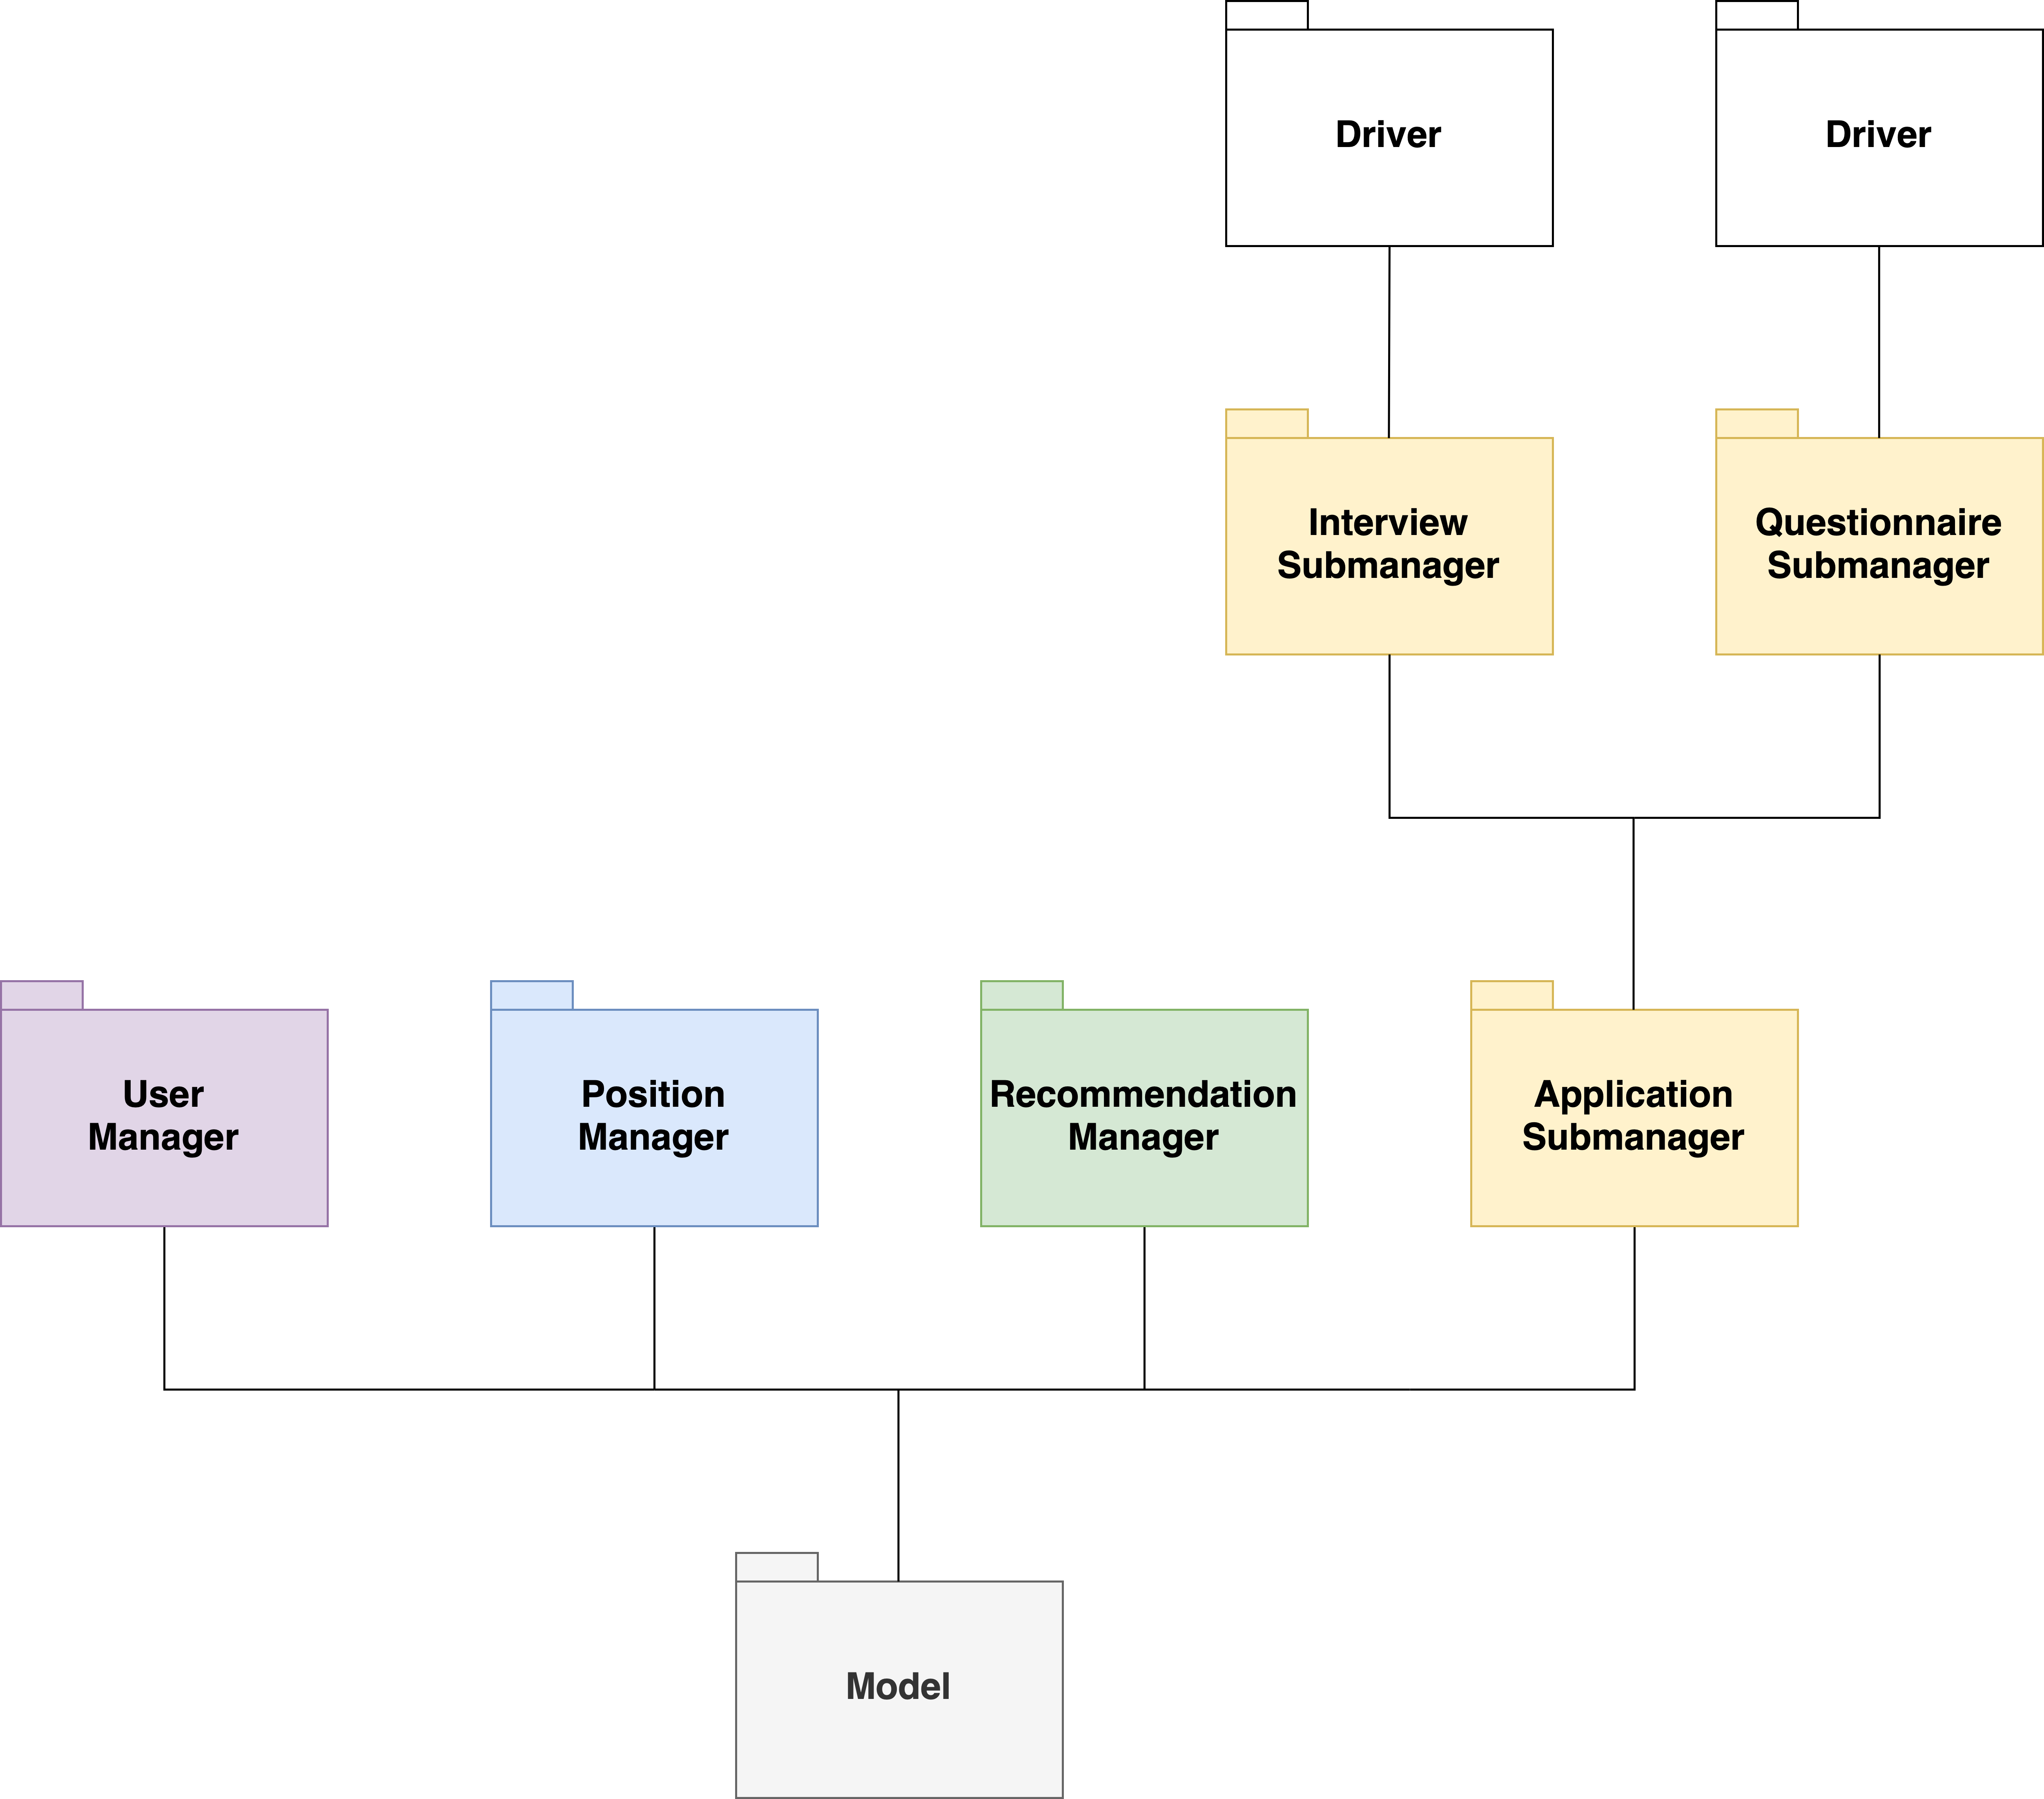
\includegraphics[width=14.5cm]{images/implementation-diagrams/step-8.png}
    \caption{Implementation step 8}
\end{figure}

\newpage
The development proceeds to step nine with the application submanagers.

\begin{figure}[h]
    \centering
    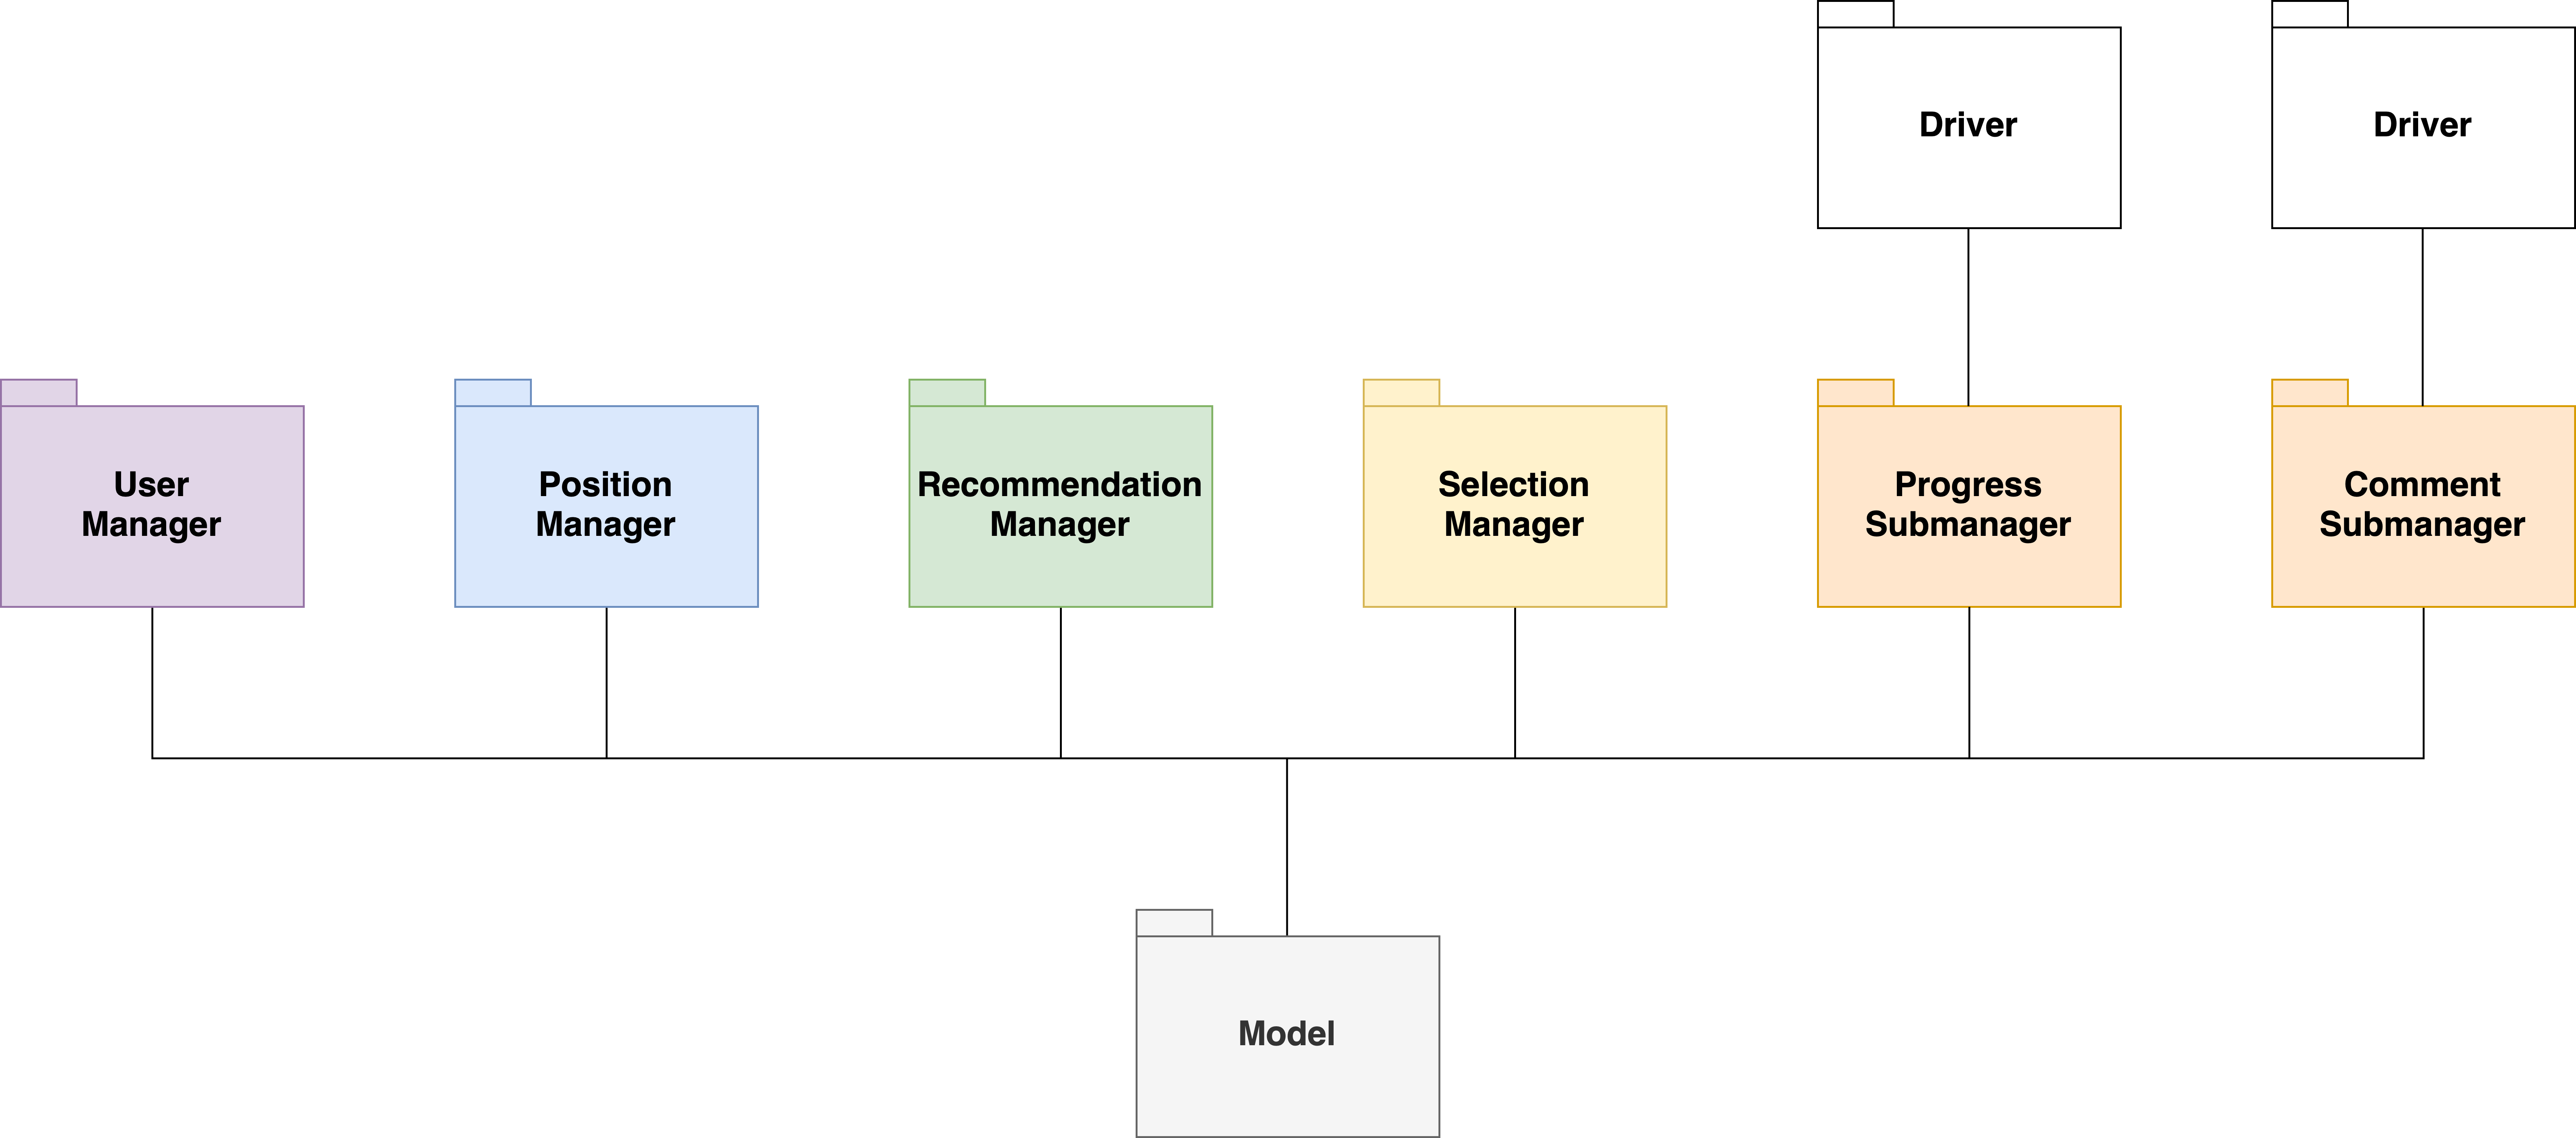
\includegraphics[width=16cm]{images/implementation-diagrams/step-9.png}
    \caption{Implementation step 9}
\end{figure}

\newpage
Step ten applies the same pattern to the notification submanagers.

\begin{figure}[h]
    \centering
    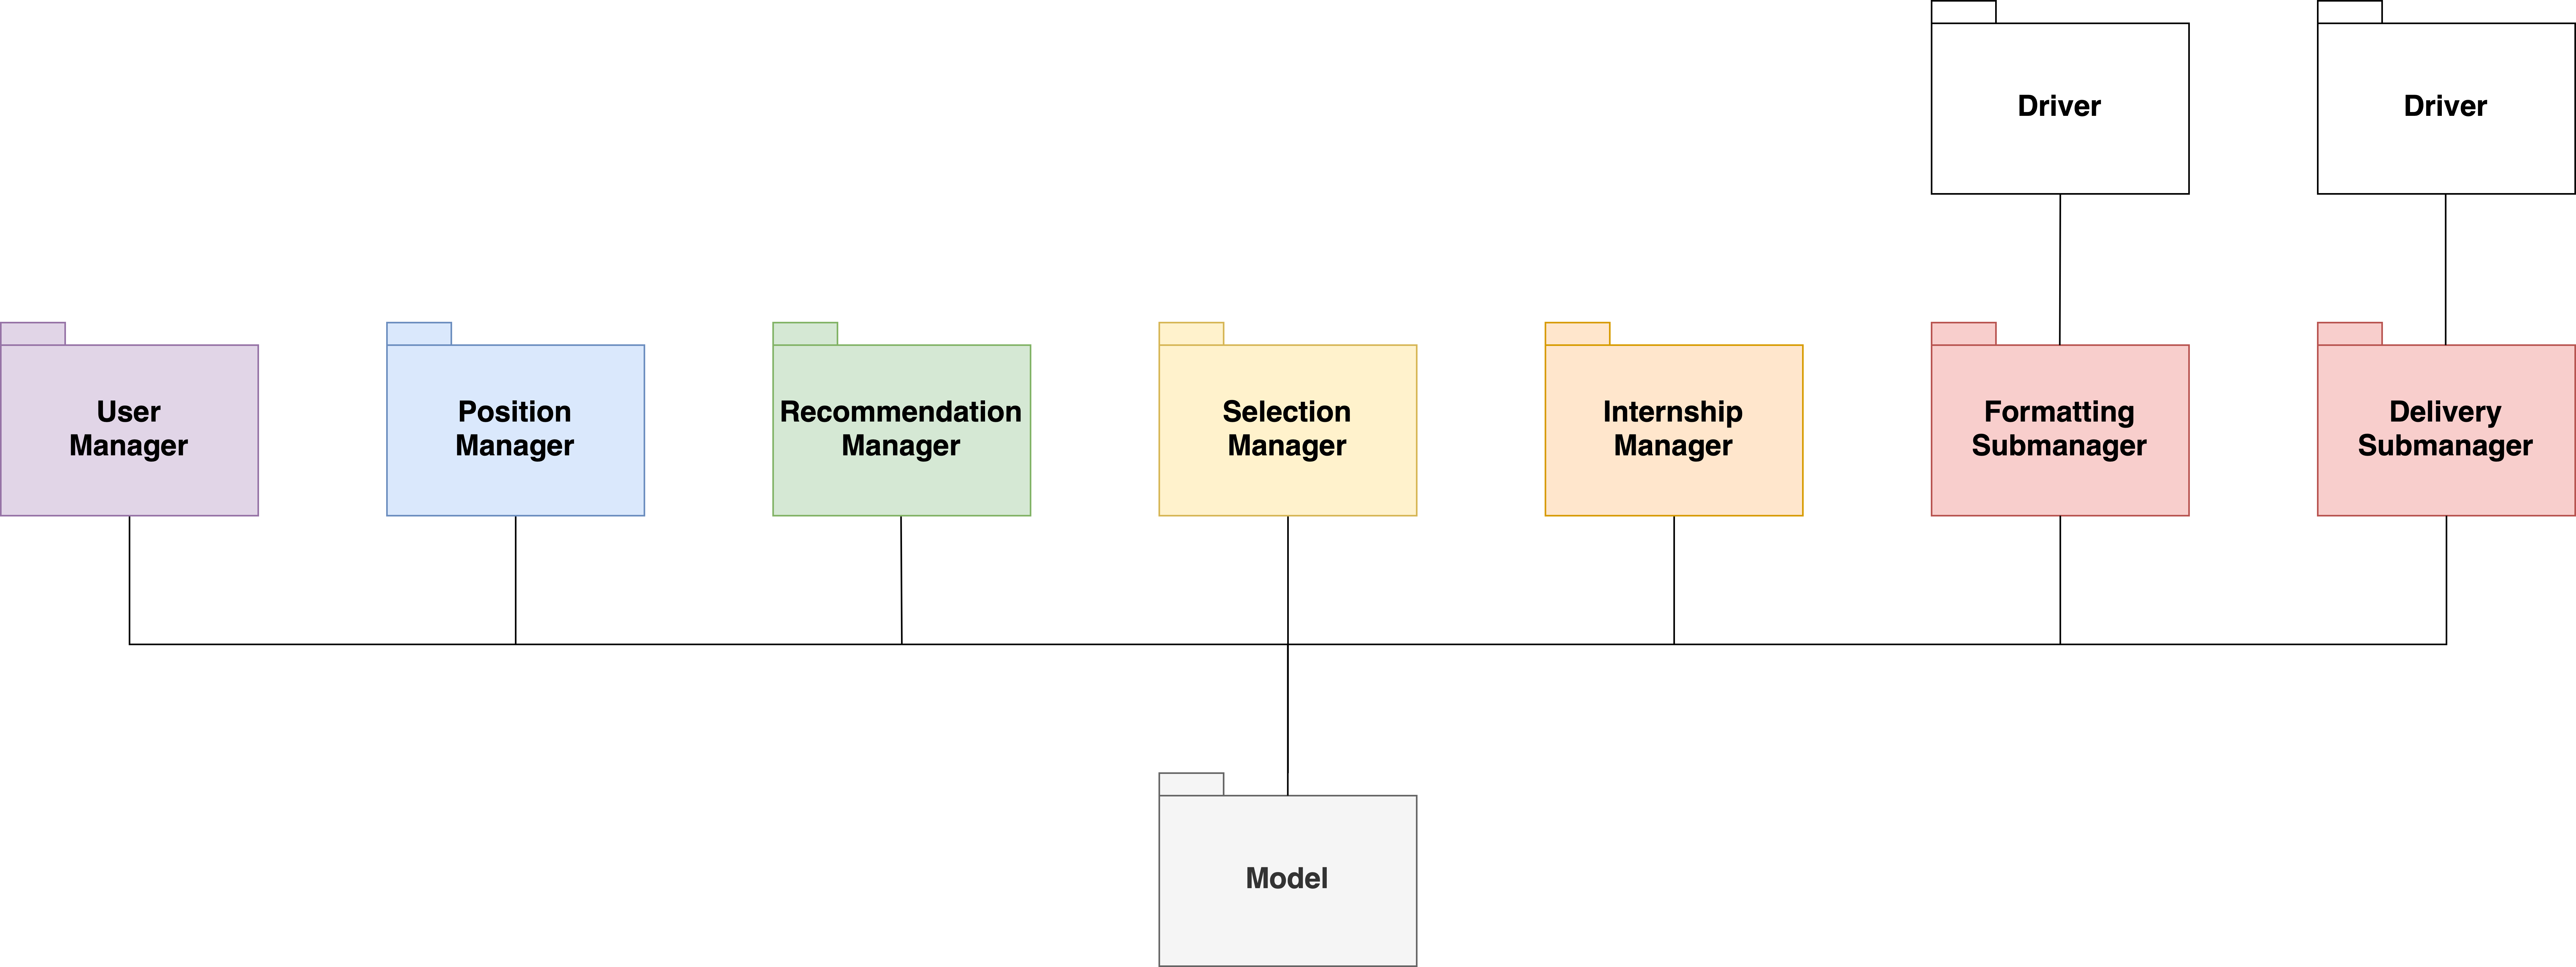
\includegraphics[width=16cm]{images/implementation-diagrams/step-10.png}
    \caption{Implementation step 10}
\end{figure}

\newpage
Note that the notification manager supports all implemented managers.

\begin{figure}[h]
    \centering
    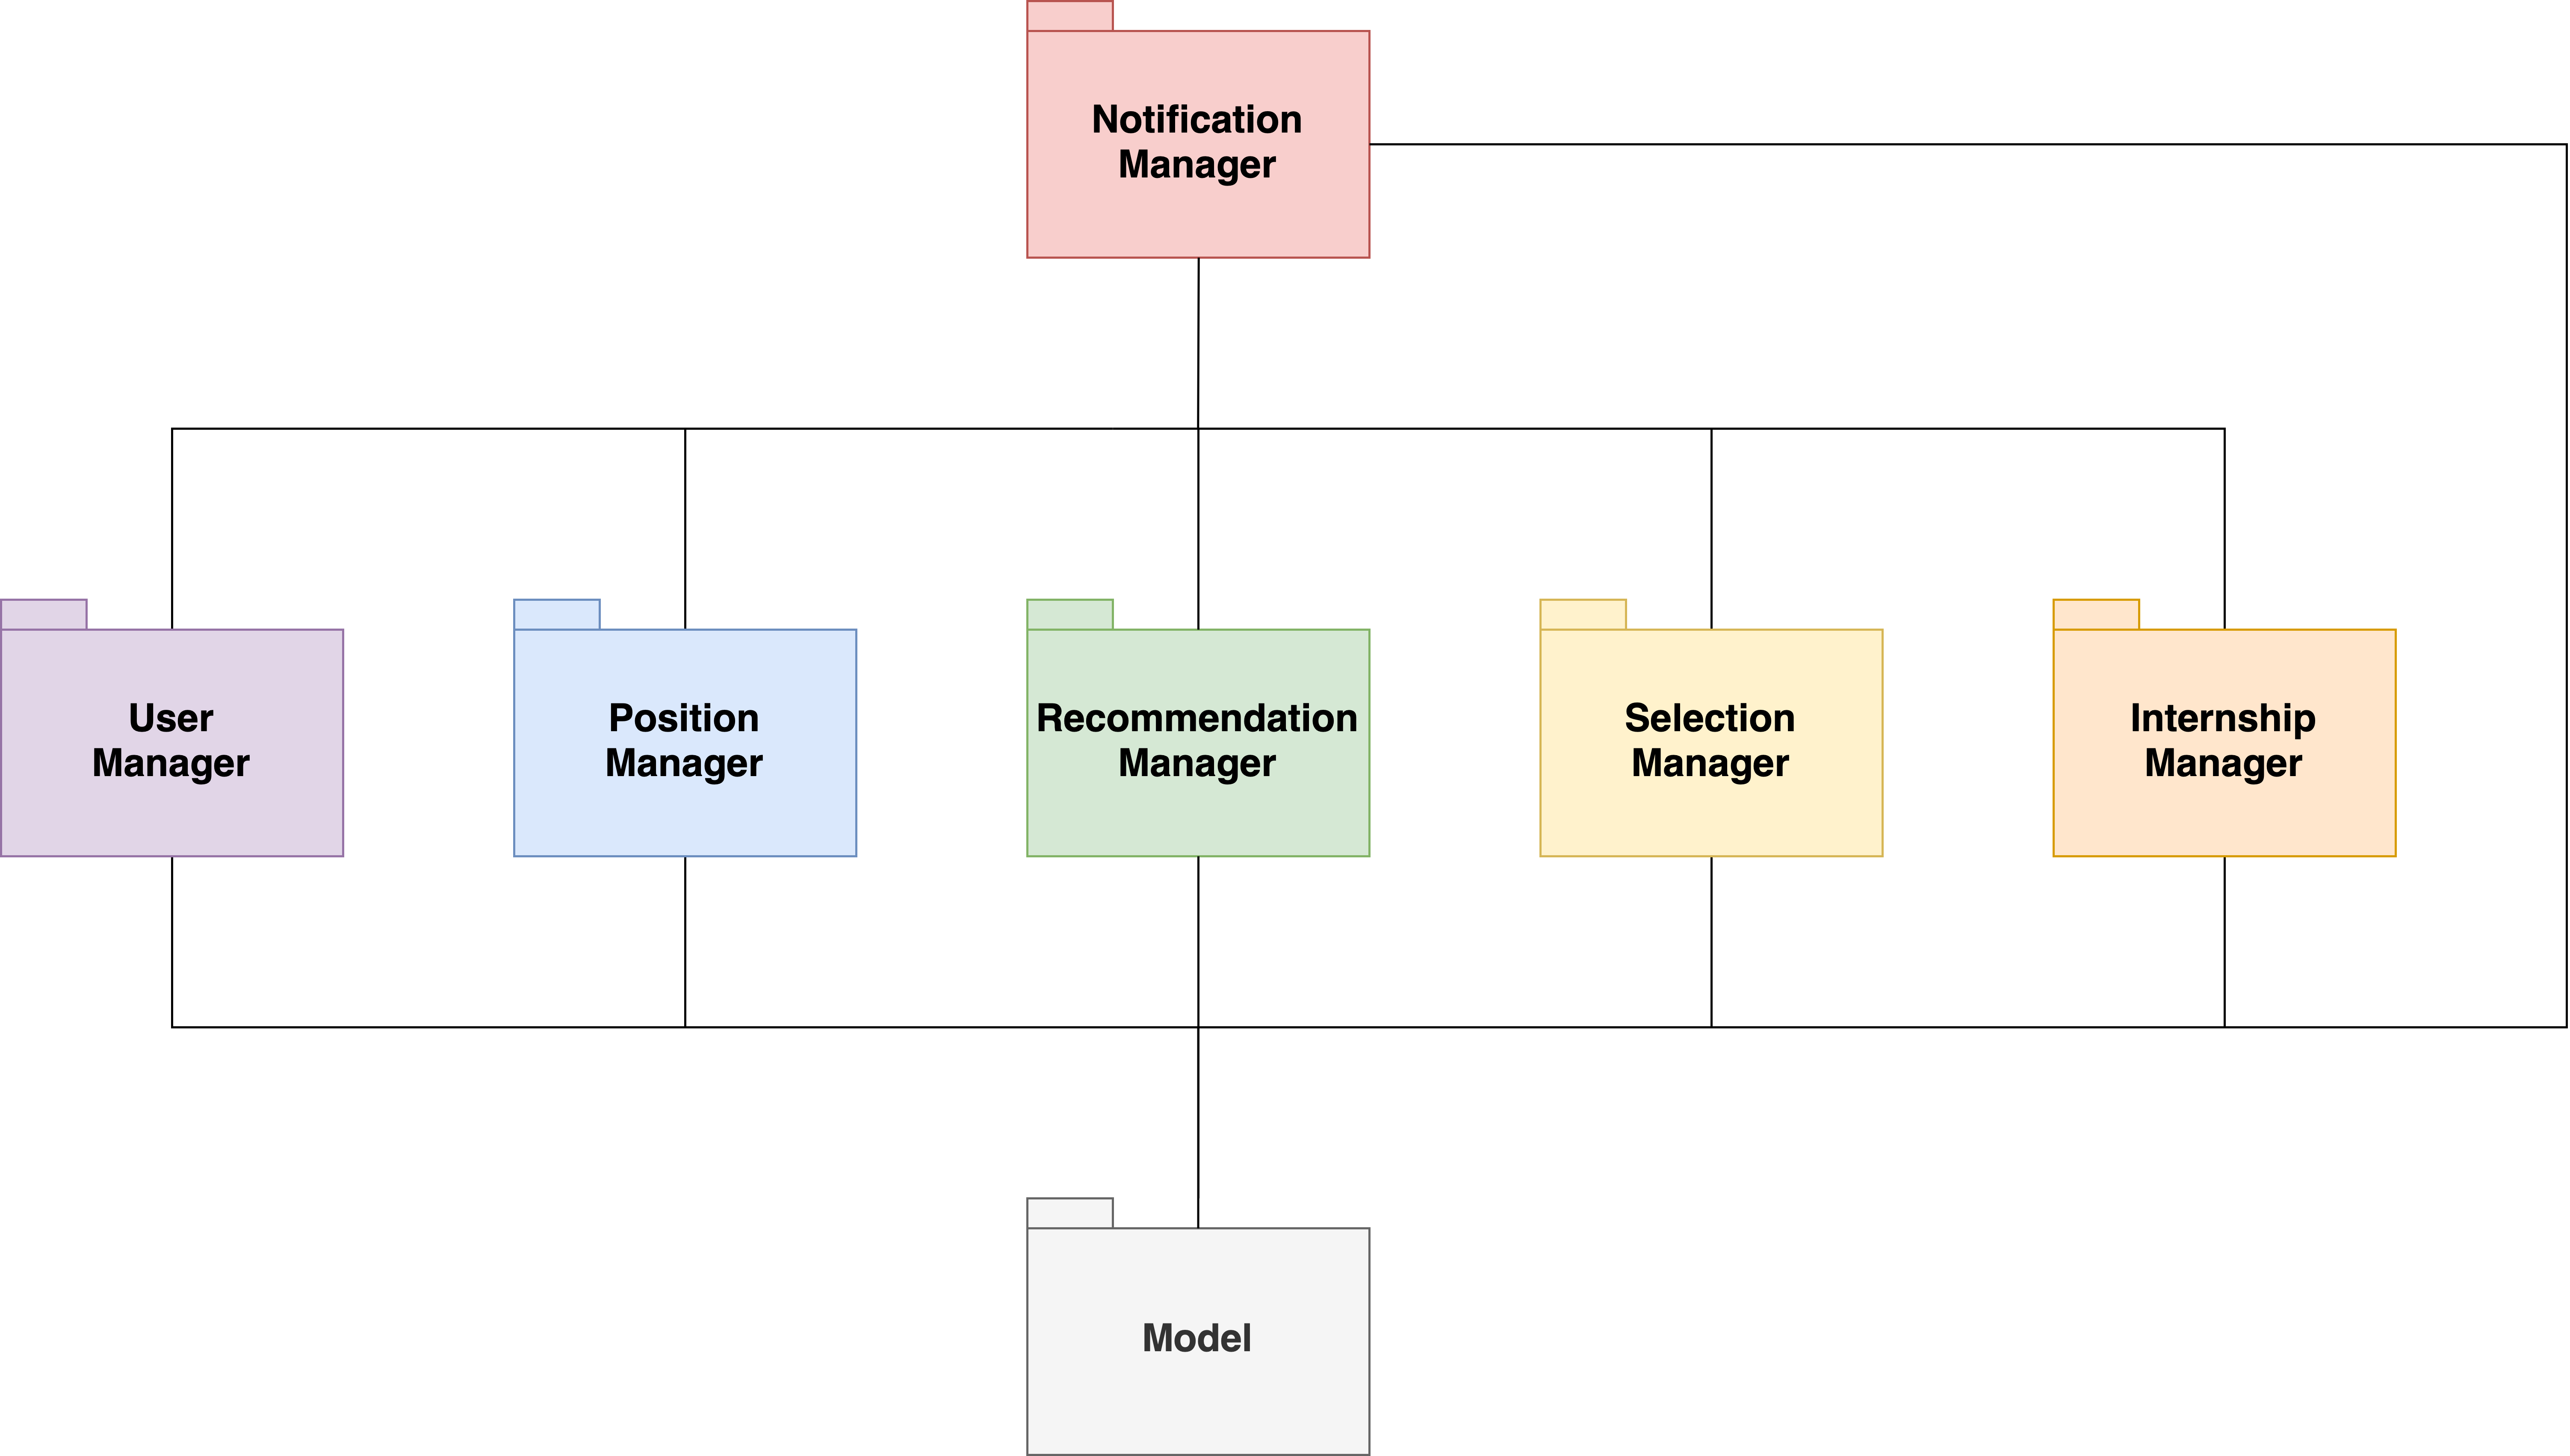
\includegraphics[width=16cm]{images/implementation-diagrams/step-11.png}
    \caption{Implementation step 11}
\end{figure}


\chapter{Workload}
This chapter quantifies the workload of the authors in writing the document.

\subsubsection{Andrea Carrara}
\renewcommand{\arraystretch}{1.5}
\begin{longtable}{|p{8.5cm}|c|}
    \hline \rowcolor{polimiblue!40}
    \textbf{Task} & \textbf{Hours} \\ \hline
    Introduction & 2  \\ \hline
    Overview & 3 \\ \hline
    Component View & 4\\ \hline
    Deployment View & 2 \\ \hline
    Runtime View & 11 \\ \hline
    Architectural Styles and Pattern & 2 \\ \hline
    Other Design Decisions & 2 \\ \hline
    Peer Review & 14 \\ \hline
    \hline \rowcolor{polimiblue!40}
    \textbf{Total} & \textbf{40} \\ \hline
\caption{Workload of Andrea Carrara}
\end{longtable}

\subsubsection{Federica Currò Dossi}
\renewcommand{\arraystretch}{1.5}
\begin{longtable}{|p{8.5cm}|c|}
    \hline \rowcolor{polimiblue!40}
    \textbf{Task} & \textbf{Hours} \\ \hline
    Component Interfaces & 8\\ \hline
    User Interface Design & 11\\ \hline
    Requirements Traceability & 2 \\ \hline
    Implementation, Integration and Test Plan & 5 \\ \hline
    Peer Review & 14 \\ \hline
    \hline \rowcolor{polimiblue!40}
    \textbf{Total} & \textbf{40} \\ \hline
\caption{Workload of Federica Currò Dossi}
\end{longtable}


\printbibliography

\listoffigures

\listoftables

\end{document}
